\PassOptionsToPackage{unicode=true}{hyperref} % options for packages loaded elsewhere
\PassOptionsToPackage{hyphens}{url}
%
\documentclass[]{book}
\usepackage{lmodern}
\usepackage{amssymb,amsmath}
\usepackage{ifxetex,ifluatex}
\usepackage{fixltx2e} % provides \textsubscript
\ifnum 0\ifxetex 1\fi\ifluatex 1\fi=0 % if pdftex
  \usepackage[T1]{fontenc}
  \usepackage[utf8]{inputenc}
  \usepackage{textcomp} % provides euro and other symbols
\else % if luatex or xelatex
  \usepackage{unicode-math}
  \defaultfontfeatures{Ligatures=TeX,Scale=MatchLowercase}
\fi
% use upquote if available, for straight quotes in verbatim environments
\IfFileExists{upquote.sty}{\usepackage{upquote}}{}
% use microtype if available
\IfFileExists{microtype.sty}{%
\usepackage[]{microtype}
\UseMicrotypeSet[protrusion]{basicmath} % disable protrusion for tt fonts
}{}
\IfFileExists{parskip.sty}{%
\usepackage{parskip}
}{% else
\setlength{\parindent}{0pt}
\setlength{\parskip}{6pt plus 2pt minus 1pt}
}
\usepackage{hyperref}
\hypersetup{
            pdftitle={Impact Malaria Data Hub Specifications},
            pdfauthor={Isaiah Nyabuto, Eric Ejimba, Cristina Lussiana},
            pdfborder={0 0 0},
            breaklinks=true}
\urlstyle{same}  % don't use monospace font for urls
\usepackage{longtable,booktabs}
% Fix footnotes in tables (requires footnote package)
\IfFileExists{footnote.sty}{\usepackage{footnote}\makesavenoteenv{longtable}}{}
\usepackage{graphicx,grffile}
\makeatletter
\def\maxwidth{\ifdim\Gin@nat@width>\linewidth\linewidth\else\Gin@nat@width\fi}
\def\maxheight{\ifdim\Gin@nat@height>\textheight\textheight\else\Gin@nat@height\fi}
\makeatother
% Scale images if necessary, so that they will not overflow the page
% margins by default, and it is still possible to overwrite the defaults
% using explicit options in \includegraphics[width, height, ...]{}
\setkeys{Gin}{width=\maxwidth,height=\maxheight,keepaspectratio}
\setlength{\emergencystretch}{3em}  % prevent overfull lines
\providecommand{\tightlist}{%
  \setlength{\itemsep}{0pt}\setlength{\parskip}{0pt}}
\setcounter{secnumdepth}{5}
% Redefines (sub)paragraphs to behave more like sections
\ifx\paragraph\undefined\else
\let\oldparagraph\paragraph
\renewcommand{\paragraph}[1]{\oldparagraph{#1}\mbox{}}
\fi
\ifx\subparagraph\undefined\else
\let\oldsubparagraph\subparagraph
\renewcommand{\subparagraph}[1]{\oldsubparagraph{#1}\mbox{}}
\fi

% set default figure placement to htbp
\makeatletter
\def\fps@figure{htbp}
\makeatother

\usepackage{etoolbox}
\makeatletter
\providecommand{\subtitle}[1]{% add subtitle to \maketitle
  \apptocmd{\@title}{\par {\large #1 \par}}{}{}
}
\makeatother
\usepackage{booktabs}
\usepackage{amsthm}
\makeatletter
\def\thm@space@setup{%
  \thm@preskip=8pt plus 2pt minus 4pt
  \thm@postskip=\thm@preskip
}
\makeatother
% https://github.com/rstudio/rmarkdown/issues/337
\let\rmarkdownfootnote\footnote%
\def\footnote{\protect\rmarkdownfootnote}

% https://github.com/rstudio/rmarkdown/pull/252
\usepackage{titling}
\setlength{\droptitle}{-2em}

\pretitle{\vspace{\droptitle}\centering\huge}
\posttitle{\par}

\preauthor{\centering\large\emph}
\postauthor{\par}

\predate{\centering\large\emph}
\postdate{\par}
\usepackage[]{natbib}
\bibliographystyle{apalike}

\title{Impact Malaria Data Hub Specifications}
\author{Isaiah Nyabuto, Eric Ejimba, Cristina Lussiana}
\date{2019-12-19}

\begin{document}
\maketitle

{
\setcounter{tocdepth}{1}
\tableofcontents
}
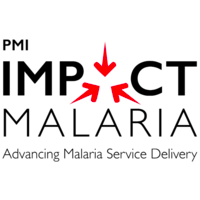
\includegraphics[width=2.78in]{./images/logo1}


\includegraphics[width=5.93in]{./images/logo2}

\hypertarget{welcome}{%
\chapter*{Welcome}\label{welcome}}
\addcontentsline{toc}{chapter}{Welcome}

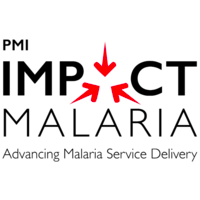
\includegraphics[width=2.78in]{./images/logo1}


\includegraphics[width=5.93in]{./images/logo2}

This is a technical guide for the IMPACT Malaria (IM) Data Hub, developed by Population Services International (PSI), to support IMPACT Malaria technical team to navigate, maintain and use the IM Data Hub.

The \href{https://imdatahub.org}{\textbf{IMPACT Malaria Data Hub}} is the IMPACT Malaria project monitoring system database for IM indicators. It is a web based database in a District Health Information Software 2 (DHIS2) instance and it houses all IM indicator data for project monitoring and use. It is primarily designed with data users in mind, and so its configuration comes with approaches specifically designed to enable monitoring and promote the use of IM data.

The IM Data Hub is used in IM countries in Africa and Asia and it collects a tremendous amount of data in the following tracks:

\begin{enumerate}
\def\labelenumi{\arabic{enumi}.}
\tightlist
\item
  Case management
\item
  Malaria in Pregnancy
\item
  Seasonal Malaria Chemoprevention
\item
  Global Technical Leadership.
\end{enumerate}

It is used by multiple partners at different levels, from Ministries of Health (MoHs), National Malaria Control Programs (NMCPs), donors like the President's Malaria Initiative (PMI), implementers (PSI, Jhpiego, University of California San Francisco (UCSF)) to track project monitoring and performance.

The IM Data Hub has two instances:

\begin{itemize}
\tightlist
\item
  A \textbf{development instance} at \href{https://dev.imdatahub.org}{dev.imdatahub.org} hosted on a ST-3 plan from BAO Systems since Nov 22nd, 2018 for prototyping, testing and piloting
\item
  A \textbf{production instance} at \href{https://imdatahub.org}{imdatahub.org} hosted on a ST-3 plan from BAO Systems since Nov 27th, 2019 for actual monitoring and reporting
\end{itemize}

This guide provides all the information and the technical specifications you need to know about the IM Data Hub. It's an all-inclusive guide on the IM Data Hub and it complements other materials on DHIS2 configuration, as well as training in the IM Data Hub.

\hypertarget{preface}{%
\chapter*{Preface}\label{preface}}
\addcontentsline{toc}{chapter}{Preface}

\hypertarget{what-is-the-im-data-hub}{%
\section{What is the IM Data Hub?}\label{what-is-the-im-data-hub}}

The Impact Maria (IM) Data Hub is a project monitoring system in DHIS2 used to collect, analyze, monitor and report Impact Malaria indicator data. It's built on DHIS2 core software, and it supports HNQIS (1.4.X) compatibility.

\hypertarget{who-should-read-this-guide}{%
\section{Who should read this guide?}\label{who-should-read-this-guide}}

This guide is aimed at two main audiences:

\begin{itemize}
\tightlist
\item
  System Administrators who are involved in the configuration, maintenance and troubleshooting the IM Data Hub,
\item
  IM Project teams and M\&E staff involved in supporting M\&E activities like data entry, reporting, data analysis and visualizations and project monitoring.
\end{itemize}

The audiences will find this guide helpful in understanding the overall system set up and how different components work together in the system.

\hypertarget{what-is-covered-in-this-guide.}{%
\section{What is covered in this guide.}\label{what-is-covered-in-this-guide.}}

The guide is divided into seven chapters:

\begin{enumerate}
\def\labelenumi{\arabic{enumi}.}
\tightlist
\item
  Introduction - offers some background information, primary setup, and how to get started on the IM Data Hub quickly.
\item
  IM Data Hub Components - explores the basic set up to provide an understanding of the different components and how they function.
\item
  Data Specification - builds on the IM Data Hub components and talks about the IM indicators and data reporting.
\item
  Metadata Specifications - Explores the data specification and IM Data Hub components to talks about what lies at the bottom, the metadata.
\item
  Security and Access Model - Explains the security mechanisms and access model implemented in the IM Data Hub.
\item
  Health Network Quality Improvement System (HNQIS) - A brief overview of the HNQIS and how to get started.
\item
  Getting help - Some guidance on how to get help in the IM Data Hub.
\item
  References
\end{enumerate}

\hypertarget{what-is-not-covered-in-this-guide.}{%
\section{What is not covered in this guide.}\label{what-is-not-covered-in-this-guide.}}

The focus of this guide is to walk you through the technical specification of the IM Data Hub. We attempt to showcase some best practices in configuring, testing, troubleshooting, reporting, monitoring, or use of data in the IM Data Hub. However, this is not a training on \href{https://academy.dhis2.org/courses/HISP/DHIS2_Level1/2015_Q1/about}{DHIS2 Foundamentals} and you need other references to master these essential skill sets.

\hypertarget{conventions}{%
\section{Conventions}\label{conventions}}

This guide follows the following abbrevations.

\begin{longtable}[]{@{}ll@{}}
\toprule
Abbreviation & In Full\tabularnewline
\midrule
\endhead
CR & Case Reporting\tabularnewline
CS & Country Specific\tabularnewline
DX & Diagnosis\tabularnewline
IM & Impact Malaria\tabularnewline
MIP & Malaria In Pregnancy\tabularnewline
PMP & Performance Management Plan\tabularnewline
RE & Reporting\tabularnewline
SMC & Seasonal Malaria Chemoprophylaxis\tabularnewline
SS & Supportive Supervision\tabularnewline
TL & Technical Leadership\tabularnewline
TR & Training\tabularnewline
TX & Treatment\tabularnewline
\bottomrule
\end{longtable}

\hypertarget{data-sets}{%
\subsection{Data Sets}\label{data-sets}}

Data set: {[}\texttt{country\ ISO\ code}{]} {[}\texttt{Data\ entry\ form\ name}{]}:

Examples:

\begin{itemize}
\tightlist
\item
  GH Supportive Supervision
\item
  CD Case Reporting
\end{itemize}

\hypertarget{data-elements}{%
\subsection{Data Elements}\label{data-elements}}

DEs: {[}\texttt{country\ ISO\ code}{]} {[}\texttt{Data\ entry\ form\ name\ abbreviation}{]} - {[}\texttt{Section\ abbreviation}{]} {[}\texttt{DE\ Form\ name}{]}:

Examples:

\begin{itemize}
\tightlist
\item
  GH CR - DX Cases confirmed
\item
  CD TL - DX Does this province have national malaria diagnostic supervision tools that adhere to global standards?
\end{itemize}

\hypertarget{indicators}{%
\subsection{Indicators}\label{indicators}}

Indicators: {[}\texttt{country\ ISO\ code}{]} {[}\texttt{PMP}{]} {[}\texttt{number}{]} - {[}\texttt{Section\ abbreviation}{]} {[}\texttt{Indicator\ name}{]}:

Example:

GH PMP 01 - DX Percentage of confirmed malaria cases

\hypertarget{intro}{%
\chapter{Introduction}\label{intro}}

\hypertarget{background}{%
\section{Background}\label{background}}

The Impact Maria (IM) Data Hub is a web-based project monitoring system used to collect, analyze, monitor and report IM indicator data. \href{https://imdpactmalaria.org}{\textbf{IMPACT Malaria}} is a five year contract funded by the US President's Malaria Initiative (PMI) to work with national malaria programs to fight malaria and save lives by strengthening diagnosis, treatment, and drug-based prevention for those most at risk, particularly children and pregnant women.

The \href{https://imdatahub.org}{\textbf{IMPACT Malaria Data Hub}} is the IMPACT Malaria project monitoring system database for IM indicators. It is a web based database in a District Health Information Software 2 (DHIS2) instance and it houses all IM indicator data for project monitoring and use. It is primarily designed with data users in mind, and so its configuration comes with approaches specifically designed to enable monitoring and promote the use of IM data.

The IM Data Hub is used in IM countries in Africa and Asia and it collects a tremendous amount of data in the following tracks:

\begin{enumerate}
\def\labelenumi{\arabic{enumi}.}
\tightlist
\item
  Case Management
\item
  Malaria in pregnancy
\item
  Seasonal Malaria Chemoprevention
\item
  Global Technical Leadership.
\end{enumerate}

It is used by multiple partners at different levels, from Ministries of Health (MoHs), National Malaria Control Programs (NMCPs), donors like the President's Malaria Initiative (PMI), implementers (PSI, Jhpiego, University of California San Francisco (UCSF)) to track project monitoring and performance.

\hypertarget{purpose}{%
\subsection{Purpose}\label{purpose}}

The IM Data Hub was developed:

\begin{enumerate}
\def\labelenumi{\arabic{enumi}.}
\tightlist
\item
  To monitor IM indicator data
\item
  Provide access to IM indicator data at district, country and global level
\item
  Enable central/global level data management
\item
  Track project progress and country performance
\item
  Promote data use for decision making
\end{enumerate}

\hypertarget{servers}{%
\subsection{Servers}\label{servers}}

The IM Data Hub has two istances:

\begin{itemize}
\tightlist
\item
  A \textbf{development instance} at \href{https://dev.imdatahub.org}{dev.imdatahub.org} hosted on a ST-3 plan from BAO Systems since Nov 22nd, 2018 for prototyping, testing and piloting. Analytics run daily at 00:00 and 12:00 UTC (EAT -3h)
\item
  A \textbf{production instance} at \href{https://imdatahub.org}{imdatahub.org} hosted on a ST-3 plan from BAO Systems since Nov 27th, 2019 for actual monitoring and reporting. Analytics run daily at 00:00 and 12:00 UTC (EAT -3h)
\end{itemize}

\hypertarget{getting-started}{%
\section{Getting Started}\label{getting-started}}

The easiest way to get started on the IM Data Hub is to log in at the dev server at \url{https://dev.imdatahub.org/} with the IM demo credentials \texttt{demoUser} - the pw is provided by your System Admin.

Countries doing data entry or testings have country specific demo accounts based on their country ISO codes - the pw is provided by your System Admin.

\begin{longtable}[]{@{}ll@{}}
\toprule
Country & username\tabularnewline
\midrule
\endhead
Congo & \texttt{CDdemo}\tabularnewline
Cameroon & \texttt{CMdemo}\tabularnewline
Ghana & \texttt{GHdemo}\tabularnewline
Kenya & \texttt{KEdemo}\tabularnewline
Mali & \texttt{MLdemo}\tabularnewline
Niger & \texttt{NEdemo}\tabularnewline
\bottomrule
\end{longtable}

\hypertarget{comp}{%
\chapter{IM Data Hub Components}\label{comp}}

\hypertarget{introduction}{%
\section{Introduction}\label{introduction}}

Now that you're already started, and you've got some essential background about the IM Data Hub, we are going to explore the details/components that form the IM Data Hub.

The IM Data Hub is not just a database: it's rather a project monitoring system, and it's meant to monitor IM indicators and support decision-makers.

Understanding the IM Data Hub components will allow you to report, analyse, and monitor IM indicators more effectively. We'll dive deeper into the components and understand how they are set up in the IM Data Hub.

This section shows you the reporting component, mainly the data sets that the IM Data Hub uses to collect indicator data. We will then walk through the data mining piece, and how the different outputs are pulled together on a dashboard for the project use.

\hypertarget{reporting-component}{%
\section{Reporting Component}\label{reporting-component}}

Reporting into the IM Data Hub to inform the IM Performance Monitoring Plan (PMP) indicators is organized through the use of data sets. A data set is simply a list of data elements that are grouped for data collection.

A data set has a reporting period and is assigned to organization units. The reporting period specifies how often the data is reported, ie. monthly or quarterly, while the organization units determine the location ``where'' the information is collected from.

The IM Data Hub has two main types of data sets:

\begin{enumerate}
\def\labelenumi{\arabic{enumi}.}
\tightlist
\item
  Global data sets that are common to more than one country (ie. IM Seasonal Malaria Chemoprevention),
\item
  Country specific data set that are specific to countries (ie. GH Case Reporting).
\end{enumerate}

The data sets are accessible through the \textbf{data entry app} (Fig. \ref{fig:data-entry-app}) and they appear as forms. They are designed to mimic the paper forms to allow ease of data entry/reporting process.

\begin{figure}

\includegraphics[width=3.28in]{./images/data-entry-app} \caption{An icon of the data entry app}\label{fig:data-entry-app}
\end{figure}

\hypertarget{global-dataset}{%
\subsection{Global data sets}\label{global-dataset}}

Global data sets are accessible to relevant countries and are meant to collect data to inform country and global PMP Indicators.

As of Dec 2019, there are five global data sets in the IM Data Hub and all of them begin with \texttt{IM} followed by the \texttt{{[}data\ set\ name{]}} as shown below in yellow (Fig \ref{fig:im-datasets}). Global data sets are divided into sections (in grey) that groups IM data elements into multiple subheadings for ease of data collection. There are five main sections:

\begin{enumerate}
\def\labelenumi{\arabic{enumi}.}
\tightlist
\item
  Diagnosis
\item
  Treatment
\item
  MIP
\item
  Technical leadership
\item
  Seasonal Malaria Chemoprevention
\end{enumerate}

\begin{figure}
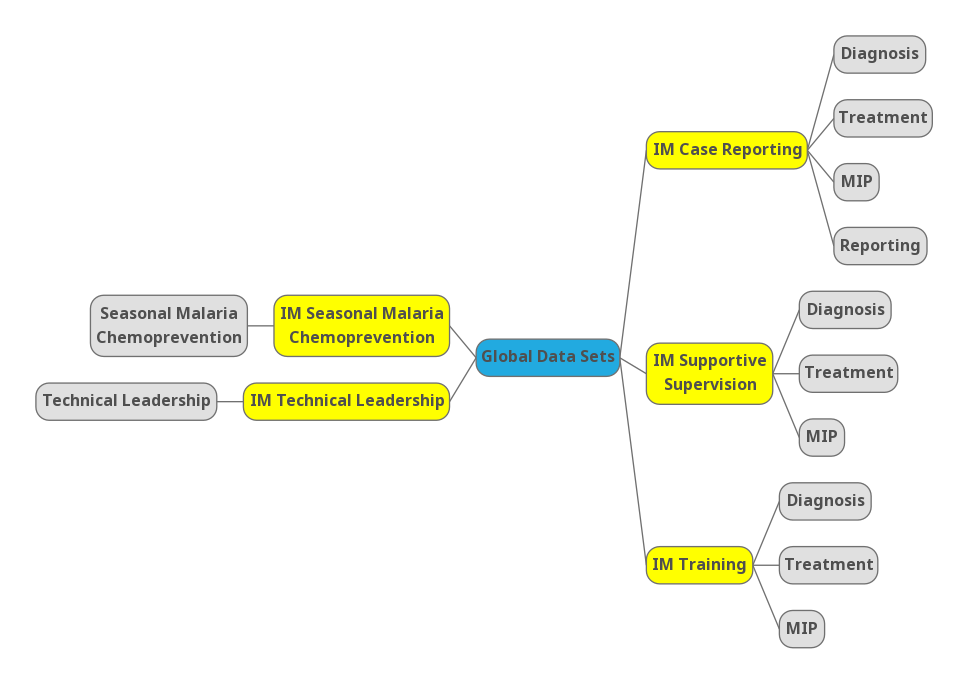
\includegraphics[width=13.47in]{./images/im datasets} \caption{Global datasets}\label{fig:im-datasets}
\end{figure}

\hypertarget{access-global-datasets}{%
\subsubsection{Accessing Global data sets}\label{access-global-datasets}}

\begin{enumerate}
\def\labelenumi{\arabic{enumi}.}
\tightlist
\item
  If you haven't already logged in yet, please log in now at:
\end{enumerate}

\href{https://imdatahub.org}{IM Data Hub demo}

\texttt{Username} :\textbf{\texttt{demoUser}} and \texttt{Password} : ask your System Admin

\begin{enumerate}
\def\labelenumi{\arabic{enumi}.}
\setcounter{enumi}{1}
\tightlist
\item
  Search for the Data Entry App from Apps
\end{enumerate}

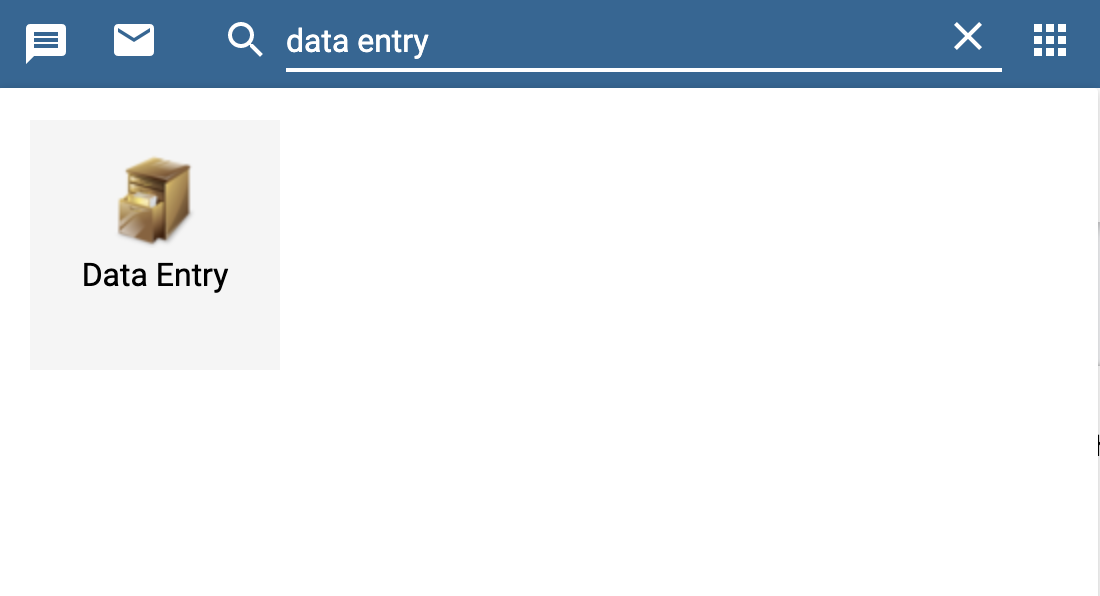
\includegraphics[width=15.28in]{./images/data-entry-app2}

\begin{enumerate}
\def\labelenumi{\arabic{enumi}.}
\setcounter{enumi}{2}
\tightlist
\item
  Click on the test world on top left if not already selected
\end{enumerate}

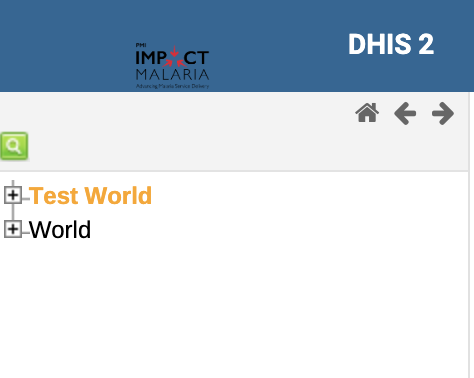
\includegraphics[width=6.58in]{./images/test-world}

\begin{enumerate}
\def\labelenumi{\arabic{enumi}.}
\setcounter{enumi}{3}
\tightlist
\item
  Select \texttt{IM\ Case\ Reporting} data set and the period to report, ie. October 2019.
\end{enumerate}

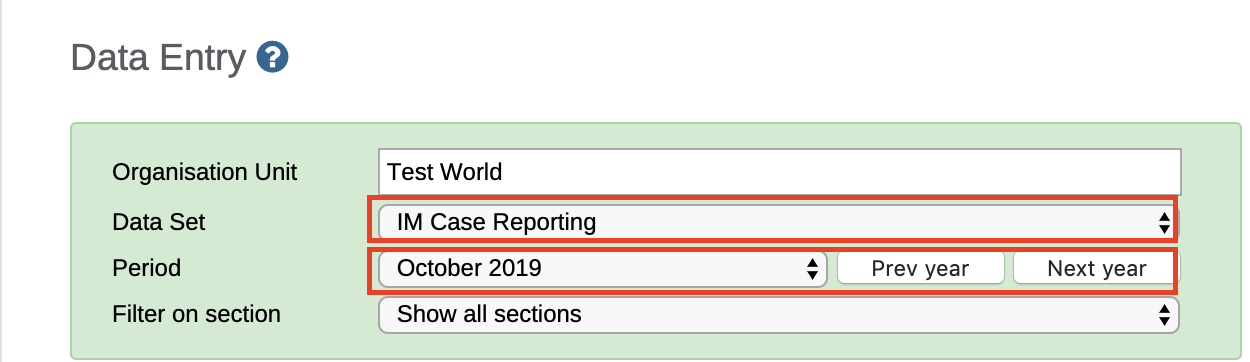
\includegraphics[width=17.36in]{./images/im-reporting}

\begin{enumerate}
\def\labelenumi{\arabic{enumi}.}
\setcounter{enumi}{4}
\tightlist
\item
  Wait for the data entry form to load, and check that you can see the same screen as in Fig \ref{fig:data-entry} below. Congratulations! You can now start reporting.

  \begin{figure}
  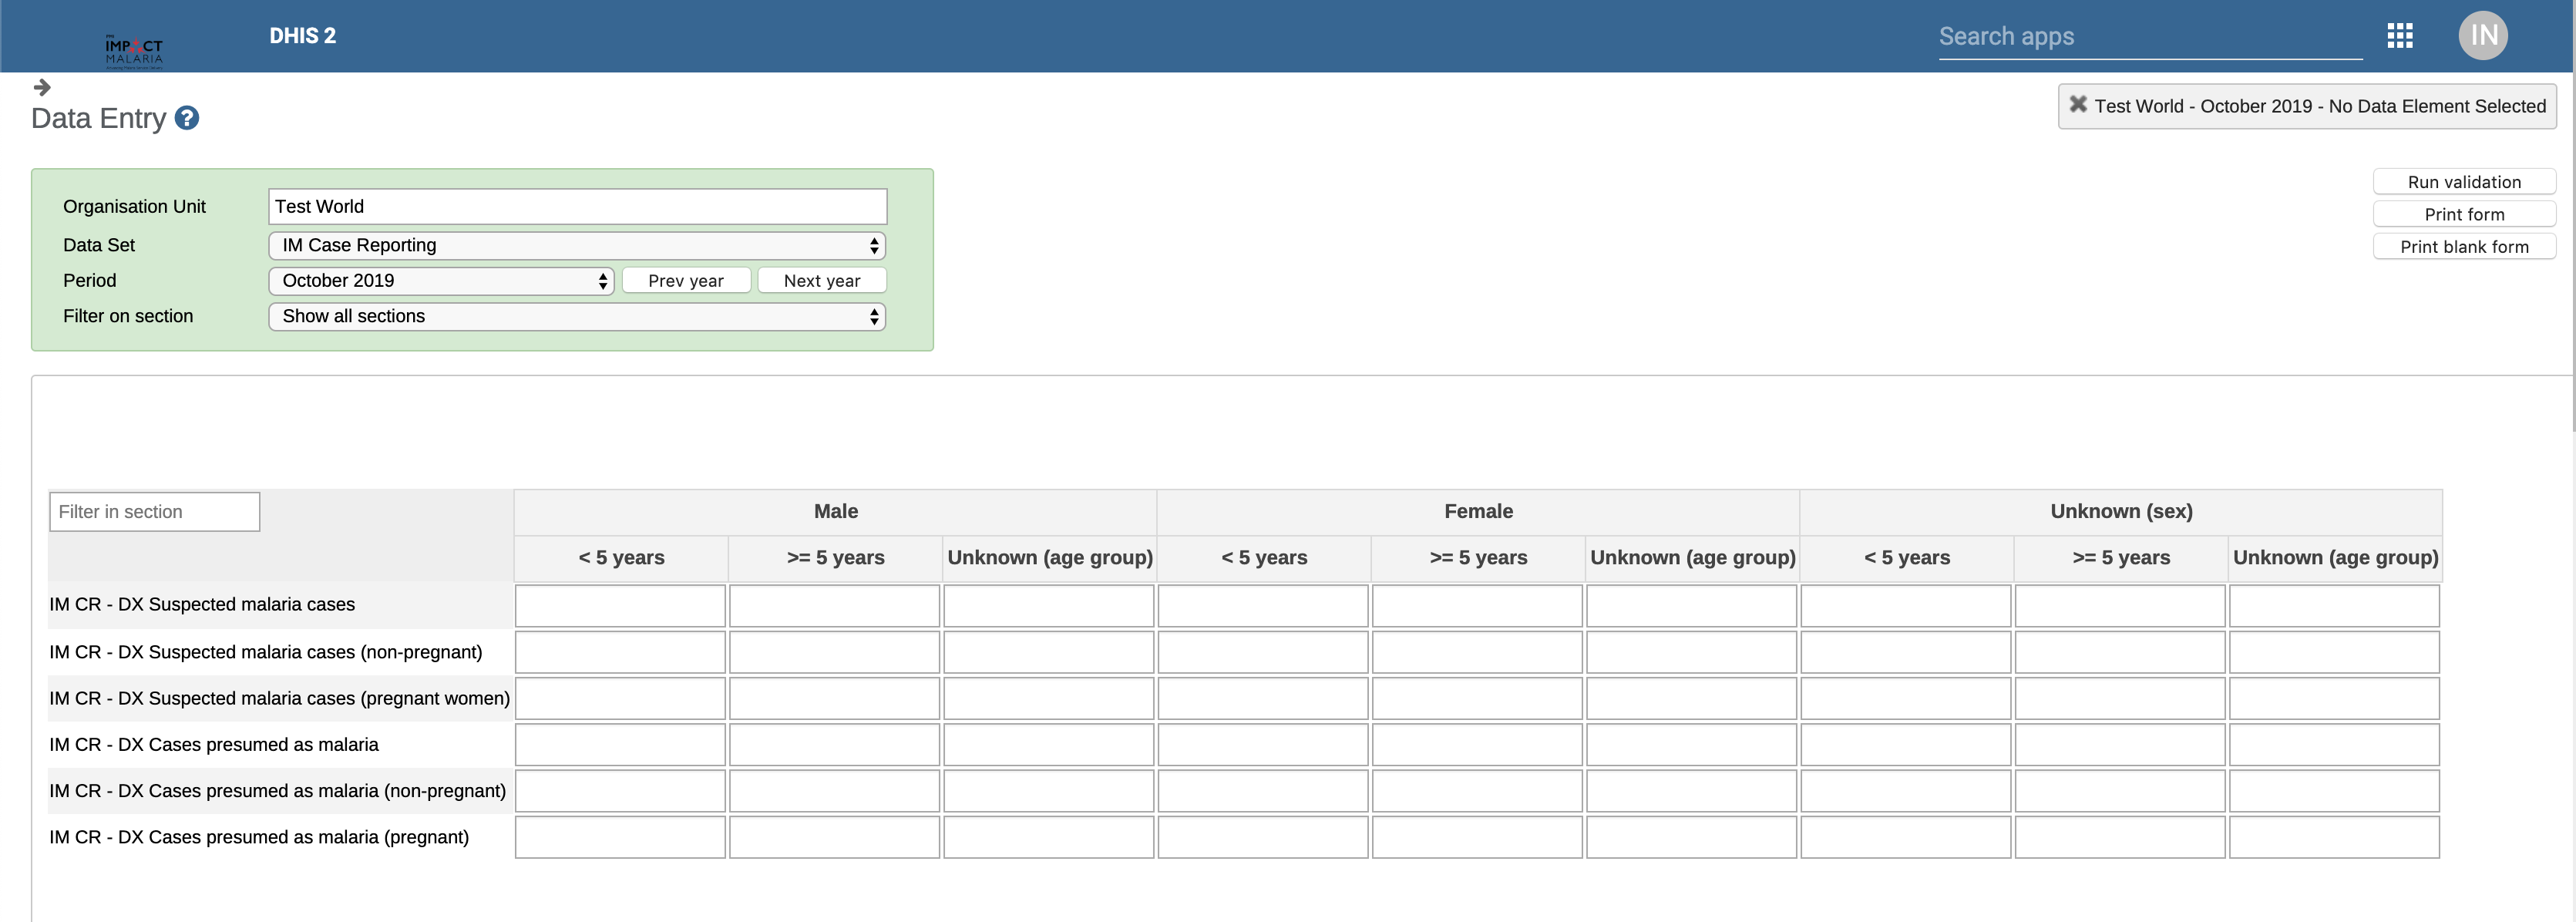
\includegraphics[width=46.42in]{./images/data-entry} \caption{IM Case Reporting Data Entry Form}\label{fig:data-entry}
  \end{figure}
\end{enumerate}

Before completing the records, please notice the \texttt{Run\ validation} button at the top right.

The complete button submits the records into the IM Data Hub.

\hypertarget{country-dataset}{%
\subsection{Country Specific Data sets}\label{country-dataset}}

Country specific data sets are used to report country's Performance Management Plan (PMP) indicators which will ultimately inform the global IM PMP indicators. They are accessible at the desired frequency of reporting (ie. annually, quarterly or monthly) and at the relevant level of data colleciton (ie. national, province, district or facility level).

Similar to the global data sets, country specific ones are organized in sections (in grey) with multiple subheadings. Fig \ref{fig:pmp-datasets}

\begin{figure}
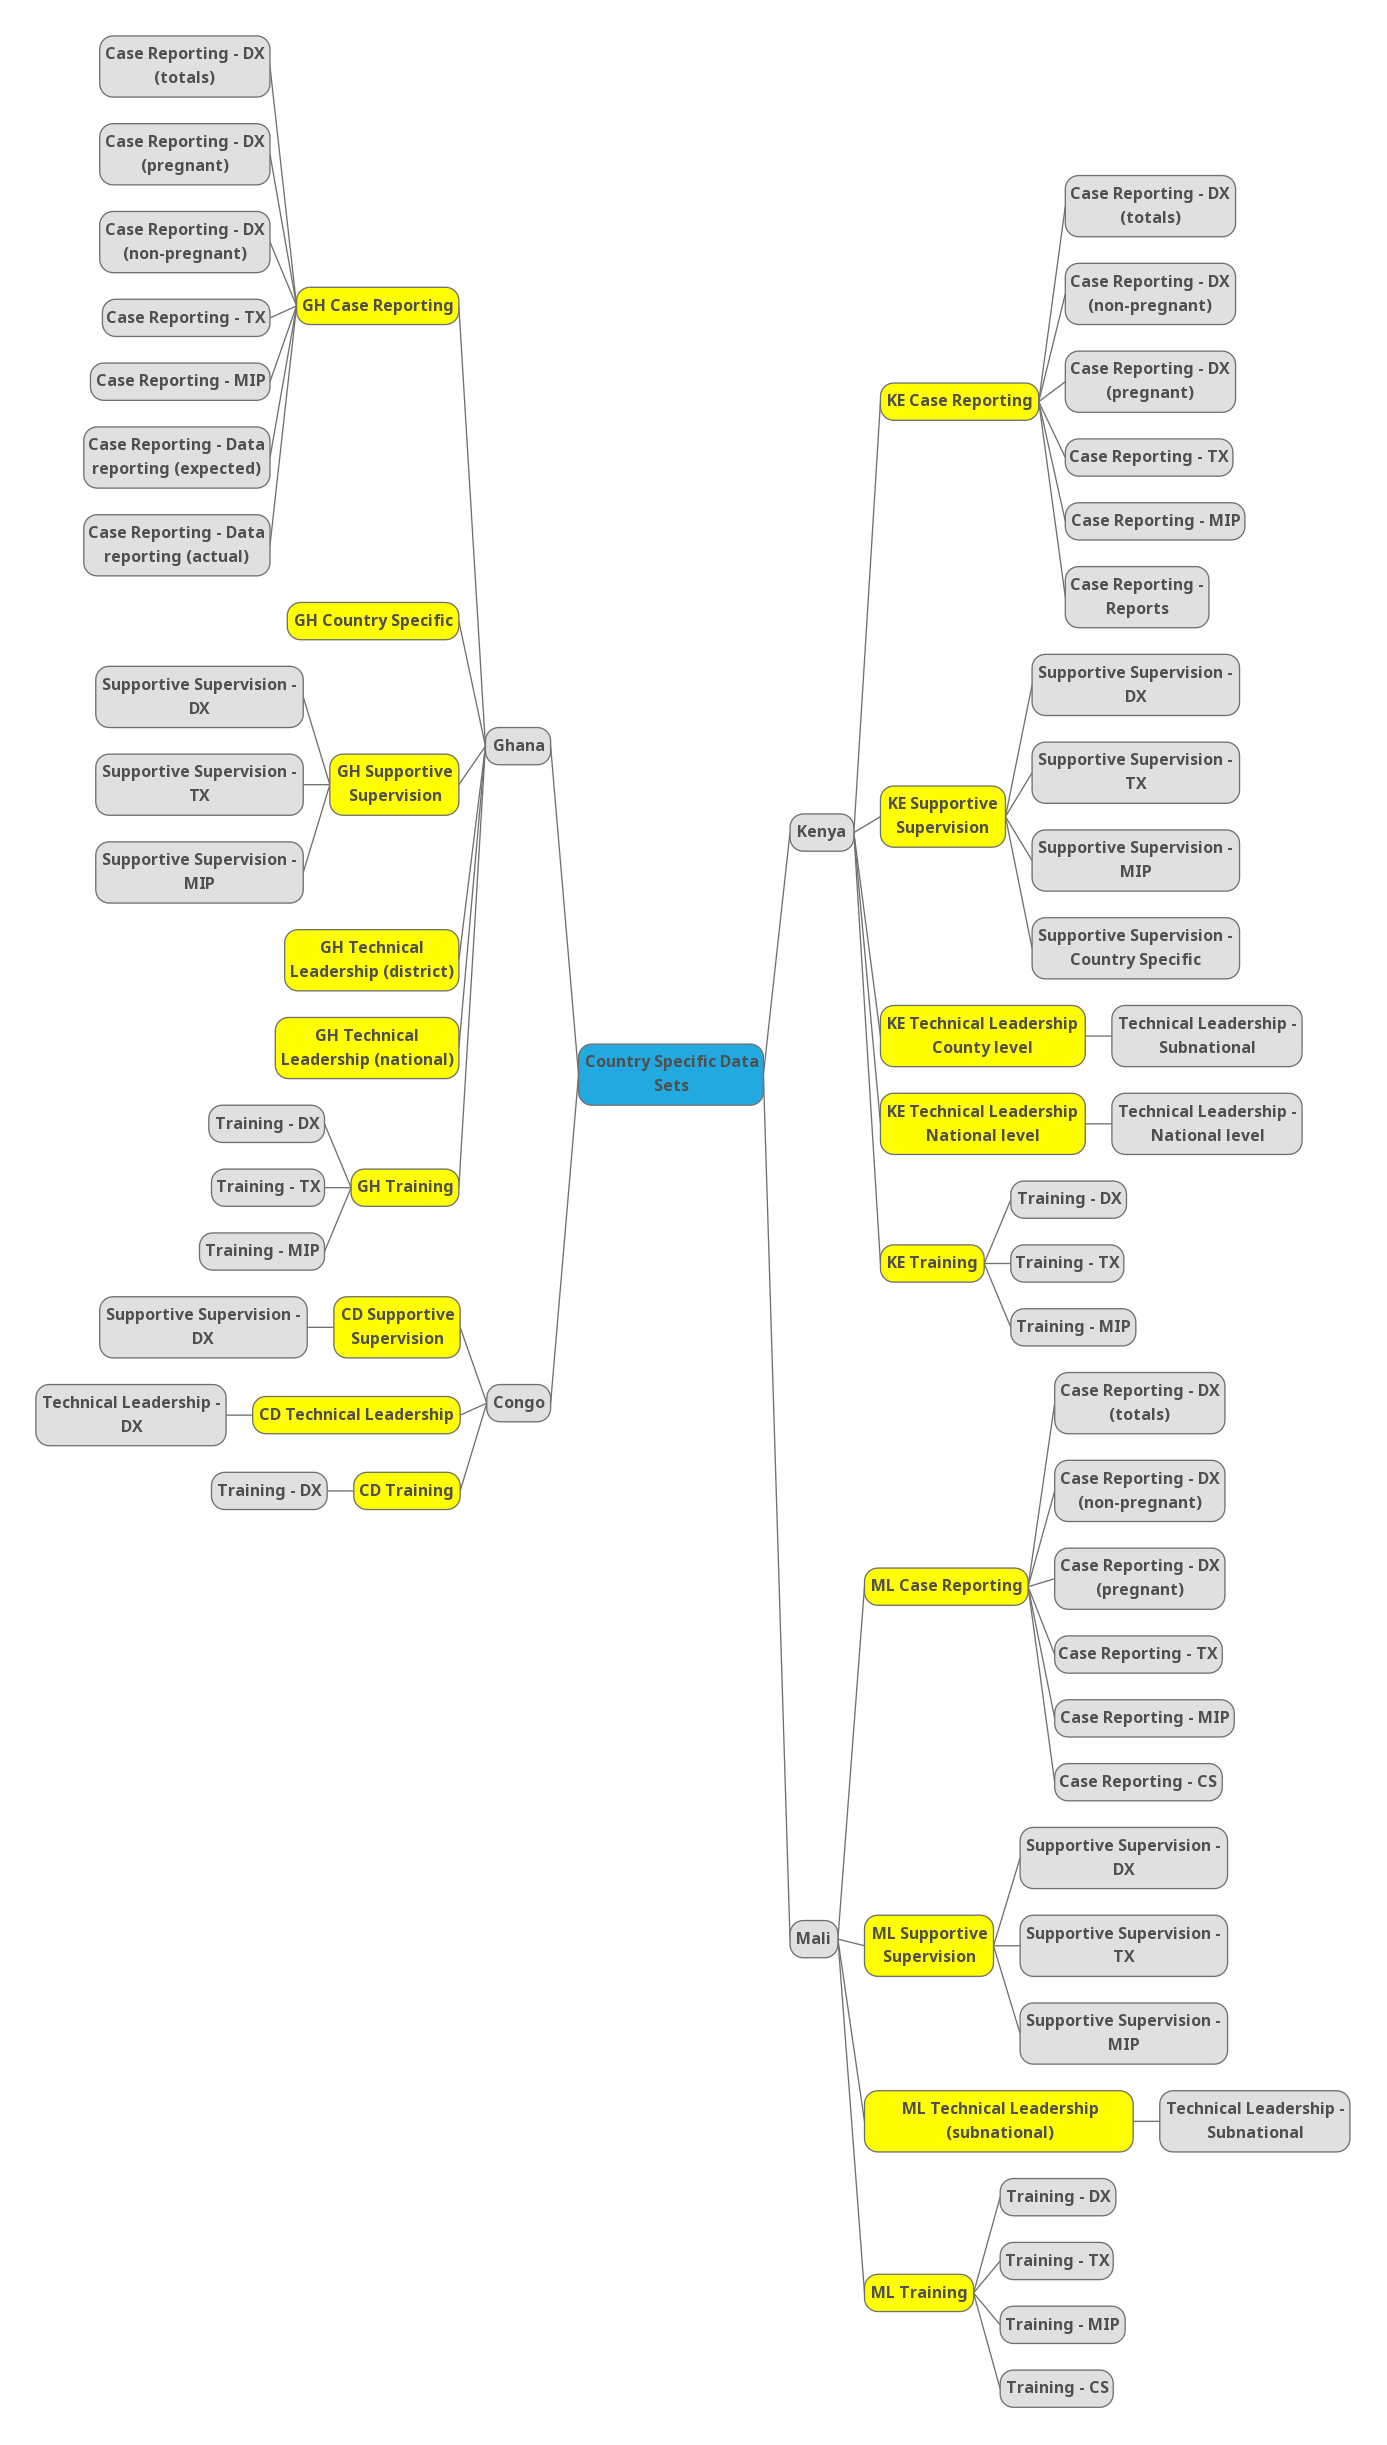
\includegraphics[width=19.26in]{./images/pmp datasets} \caption{Country Specific Datasets}\label{fig:pmp-datasets}
\end{figure}

\hypertarget{accessing-country-specific-data-sets}{%
\subsubsection{Accessing Country Specific Data sets}\label{accessing-country-specific-data-sets}}

\begin{enumerate}
\def\labelenumi{\arabic{enumi}.}
\item
  Follow the same steps in section \ref{access-global-datasets} to launch the data entry app. Ensure you are looged in with your country demo account (ie. \texttt{Username} :\textbf{\texttt{GHdemo}} and \texttt{Password} : ask your System Admin).
\item
  On the left bar, select the relevant org units you want to report from.
\item
  Select the relevant data set (ie. \texttt{{[}Country\ ISO{]}\ Case\ Reporting}) and the period to report (ie. October 2019).
\item
  Wait for the form to load.
\end{enumerate}

For some countries like \texttt{Kenya}, \texttt{Ghana} and \texttt{Mali}, the reporting process for some data sets (ie. \texttt{{[}Country\ ISO{]}\ Case\ Reporting}) is automated through scripts.

\hypertarget{data-mining-component}{%
\section{Data Mining Component}\label{data-mining-component}}

Once the data is collected or loaded into the IM Data Hub, it then becomes available for data mining. Data mining is a technical process that involves the extraction and analysis of data to generate information.

The data mining component provides tools for enabling the extraction and analysis of the IM PMP indicator data. The information collected through the data elements which compose the global and country specific data sets is pulled into global and country specific PMP indicators. Both the data elements which compose the global and country specific data sets and the global and country specific PMP indicators can be analysed and visualized in the DHIS2 analytics apps.

\begin{enumerate}
\def\labelenumi{\arabic{enumi}.}
\tightlist
\item
  Pivot Tables - extracts data in a tabular format and enables the ability to pivot data elements and indicators,
\item
  Data Visualizer - generates a variety of charts like standard line, bar charts, pie charts, etc, to pivot data elements and indicators,
\item
  Maps - gives the ability to visualize IM data elements and indicaotrs on a map.
\end{enumerate}

\hypertarget{pivot}{%
\subsection{Pivot Table}\label{pivot}}

If you are familiar with Excel, you are probably aware of ``pivoting'' as the ability to summarize data on tables in multiple dimensions. Excel Pivot Tables have inspires the DHIS2 Pivot Table app.

Pivot Table offers quick access to IM data in a tabular format. It allows the ability to `pivot' data in several dimensions, such as indicators, data elements, periods, and organization units.

In the following subsection, we are going to access and tabulate a sample of IM indicator data using the Pivot Table app.

As an example, we tabulate and pivot \texttt{IM\ Confirmed\ vs.\ Suspected\ Malaria\ Cases} for last 12 months at the global level (world).

\begin{enumerate}
\def\labelenumi{\arabic{enumi}.}
\tightlist
\item
  Please refresh your browser or login with the demo account below if you have not.
\end{enumerate}

\href{https://imdatahub.org}{IM Data Hub demo}

\texttt{Username} :\textbf{\texttt{demoUser}} and \texttt{Password} : ask your System Admin

\begin{enumerate}
\def\labelenumi{\arabic{enumi}.}
\setcounter{enumi}{1}
\item
  From Apps select or search for Pivot Tables

  \begin{figure}
  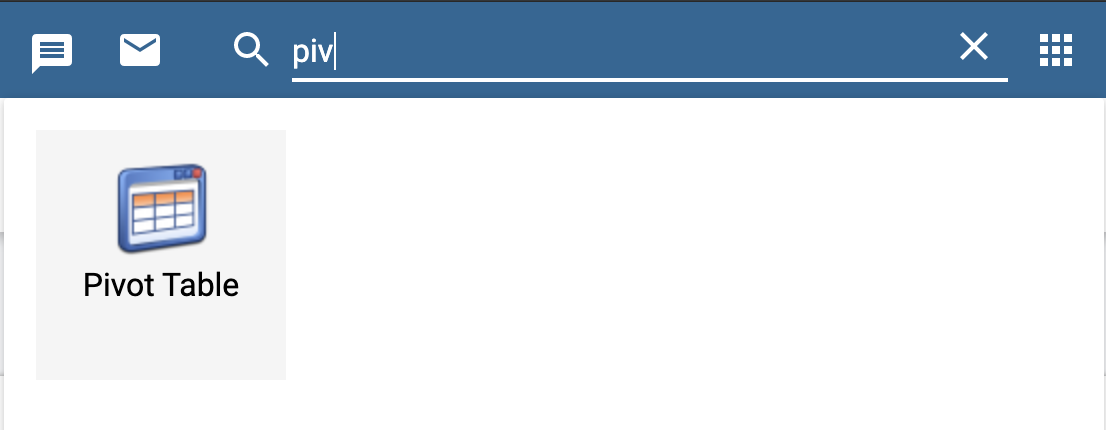
\includegraphics[width=15.36in]{./images/pivot-table} \caption{Searching Pivot Table App}\label{fig:pivot-table}
  \end{figure}
\item
  Click to launch the app
\item
  From the indicator group on your left, select IM PMP indicators and then search \% of confirmed case and \% of suspected malaria cases
\item
  Make sure you pull all the PMP indicators to the right side

  \begin{figure}
  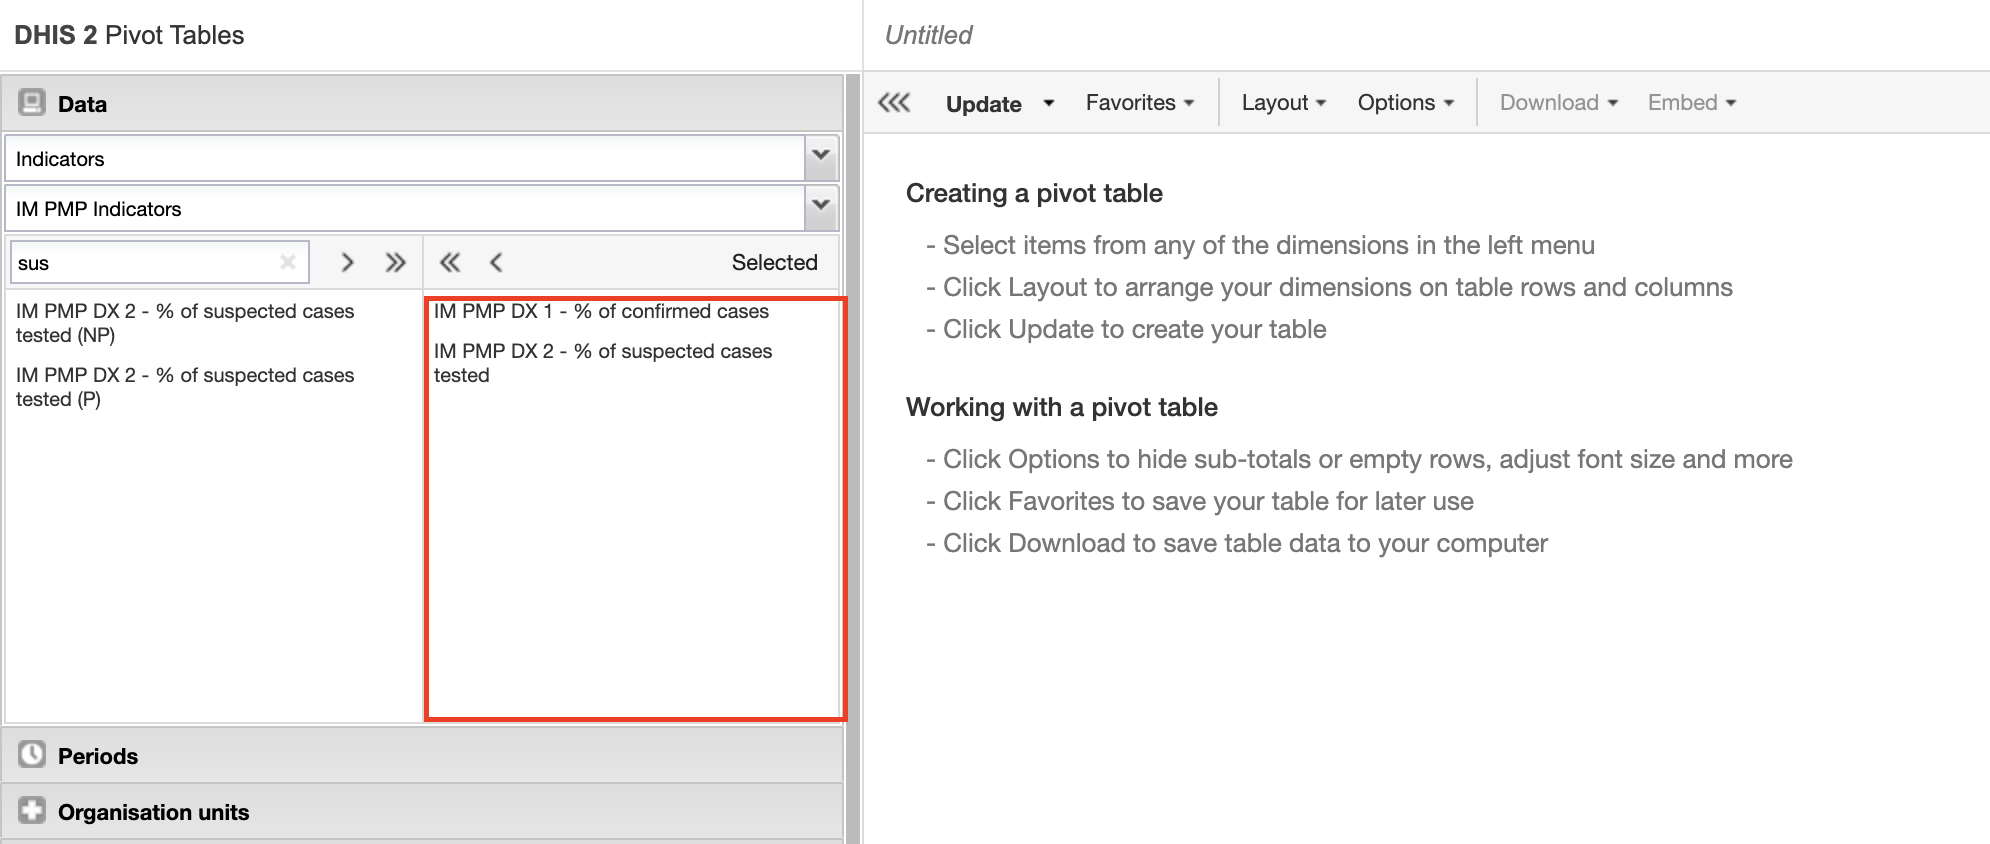
\includegraphics[width=27.64in]{./images/pivot-table2} \caption{Selecting Indicators in the Pivot Table}\label{fig:pivot-table2}
  \end{figure}
\item
  Open the organisation unit tab and select world

  \begin{figure}
  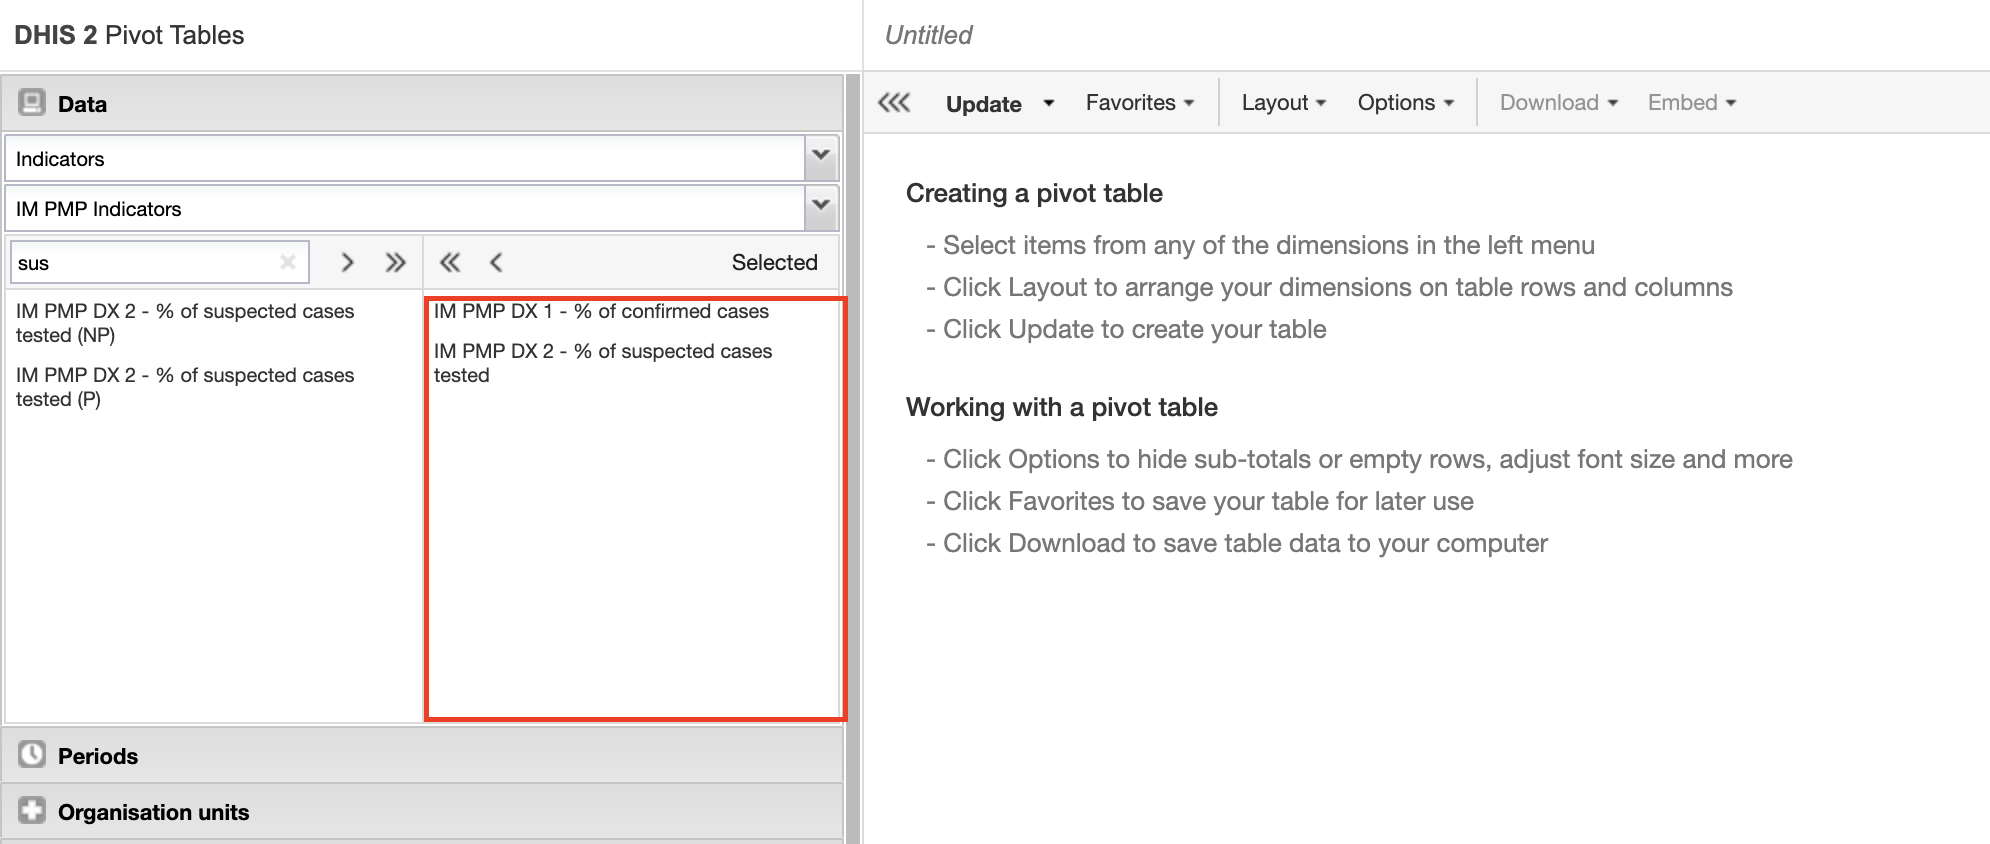
\includegraphics[width=27.64in]{./images/pivot-table2} \caption{Selecting the organisation unit}\label{fig:pivot-table4}
  \end{figure}
\end{enumerate}

\begin{quote}
At least three dimensions must be specified: what, when and where in the pivot table.
\end{quote}

\begin{enumerate}
\def\labelenumi{\arabic{enumi}.}
\setcounter{enumi}{6}
\tightlist
\item
  Click on the update button to generate the report. Check that you can see a table like this one (fig 8). Congratulations! We have tabulated our report.

  \begin{figure}
  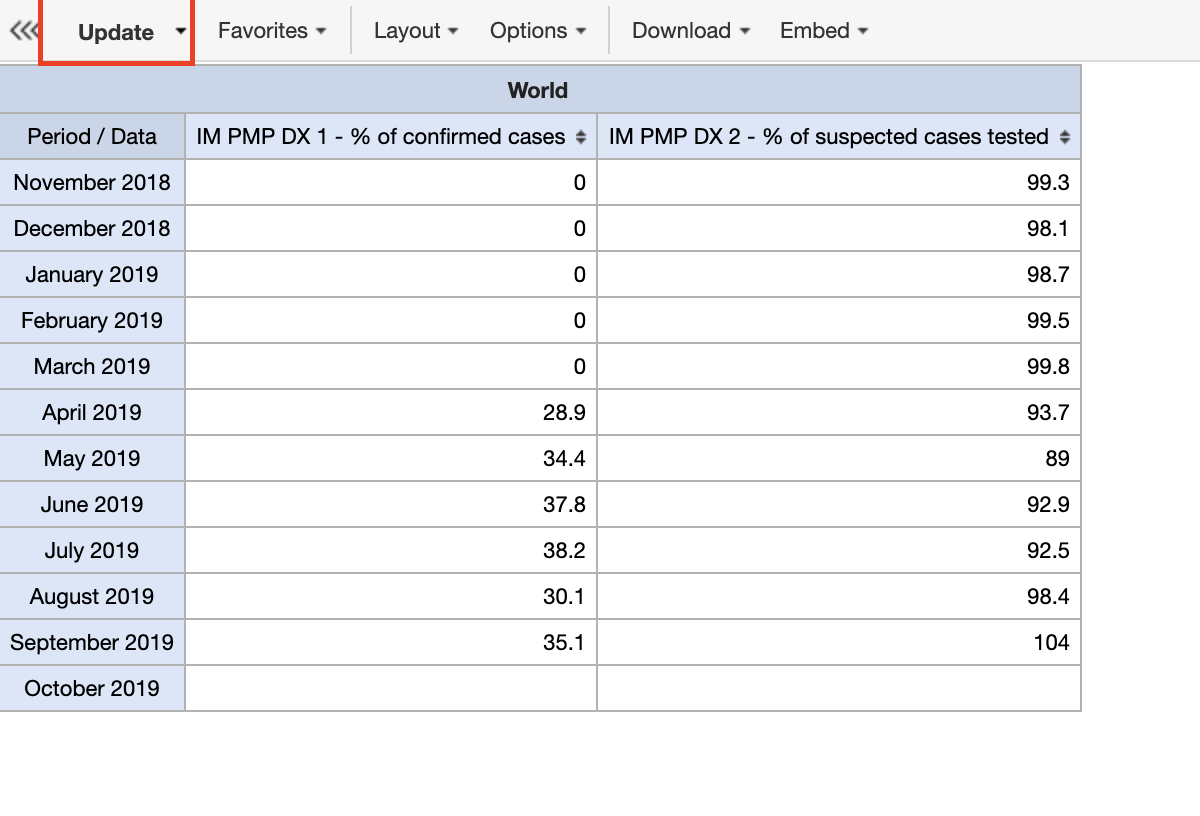
\includegraphics[width=16.67in]{./images/pivot-table3} \caption{Updating the Pivot Table}\label{fig:pivot-table3}
  \end{figure}
\end{enumerate}

\begin{quote}
Save the table as \texttt{IM\ PMP\ -\ \%\ of\ confirmed\ vs\ suspected\ cases\ last\ 12\ months,\ global}.
\end{quote}

\hypertarget{best-practices-tips-tricks}{%
\subsubsection{Best practices, tips \& tricks}\label{best-practices-tips-tricks}}

\begin{enumerate}
\def\labelenumi{\arabic{enumi}.}
\tightlist
\item
  Hide empty rows/columns is a very useful Pivot Table option when analysing data across many org units or periods with gaps in the data,
\item
  Sort your table quickly by clicking on the sort symbol inside the column header cells,
\item
  You must always save your table as a favourite before you can add it to your dashboard or share it with colleagues,
\item
  You can add color legends to your table (coloring of cells based on their values) under Options. Multiple legends can now be assigned within the same table and are created in the ``Legends'' portion of the maintenance app.
\end{enumerate}

Next we will create a chart of these using the data visualizer app.

\hypertarget{visualizer}{%
\subsection{Data Visualizer}\label{visualizer}}

Data Visualizer allows you to generate various charts, including bar charts, line graphs, pie charts, etc., directly in the IM Data Hub. They follow the same design and logic as the Pivot Table app, but they don't allow for a dimensional analysis which includes more than one factor.

\begin{enumerate}
\def\labelenumi{\arabic{enumi}.}
\tightlist
\item
  The easiest way to visualize the table in a chart is to open this table as a chart Fig. \ref{fig:visualizer}.

  \begin{figure}
  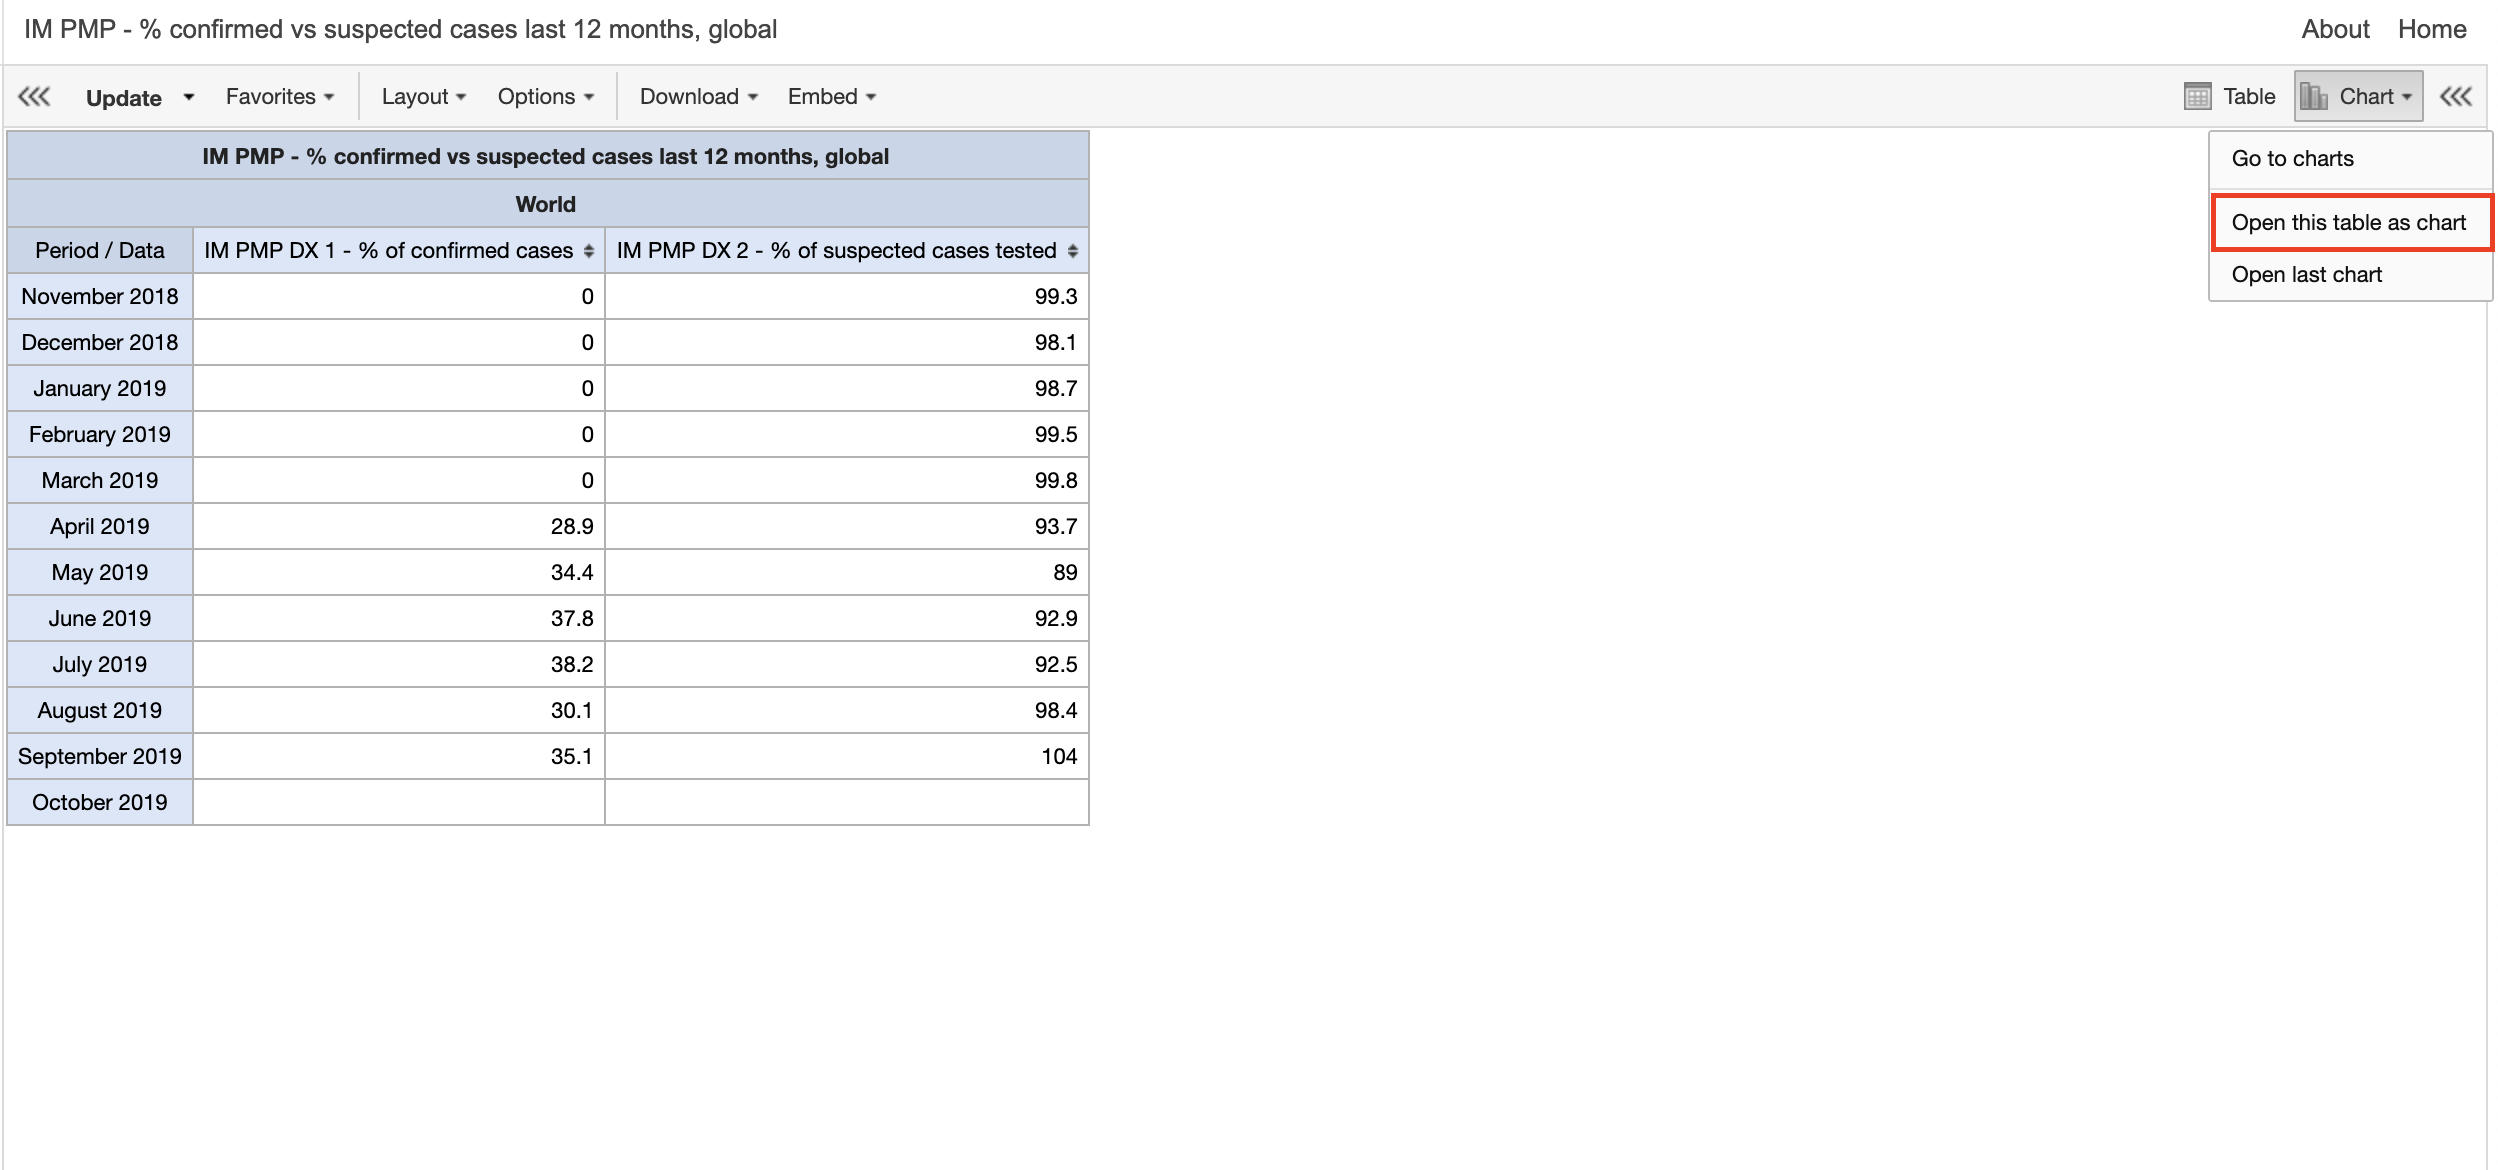
\includegraphics[width=34.69in]{./images/visualizer} \caption{Opening this table As a Chart}\label{fig:visualizer}
  \end{figure}
\item
  You can as well navigate directly to the Data Visualizer app by selecting the first option \texttt{Go\ to\ charts} or launching it form the apps menu. We will open ours as chart. Check that you see a chart as in (fig 10).

  \begin{figure}
  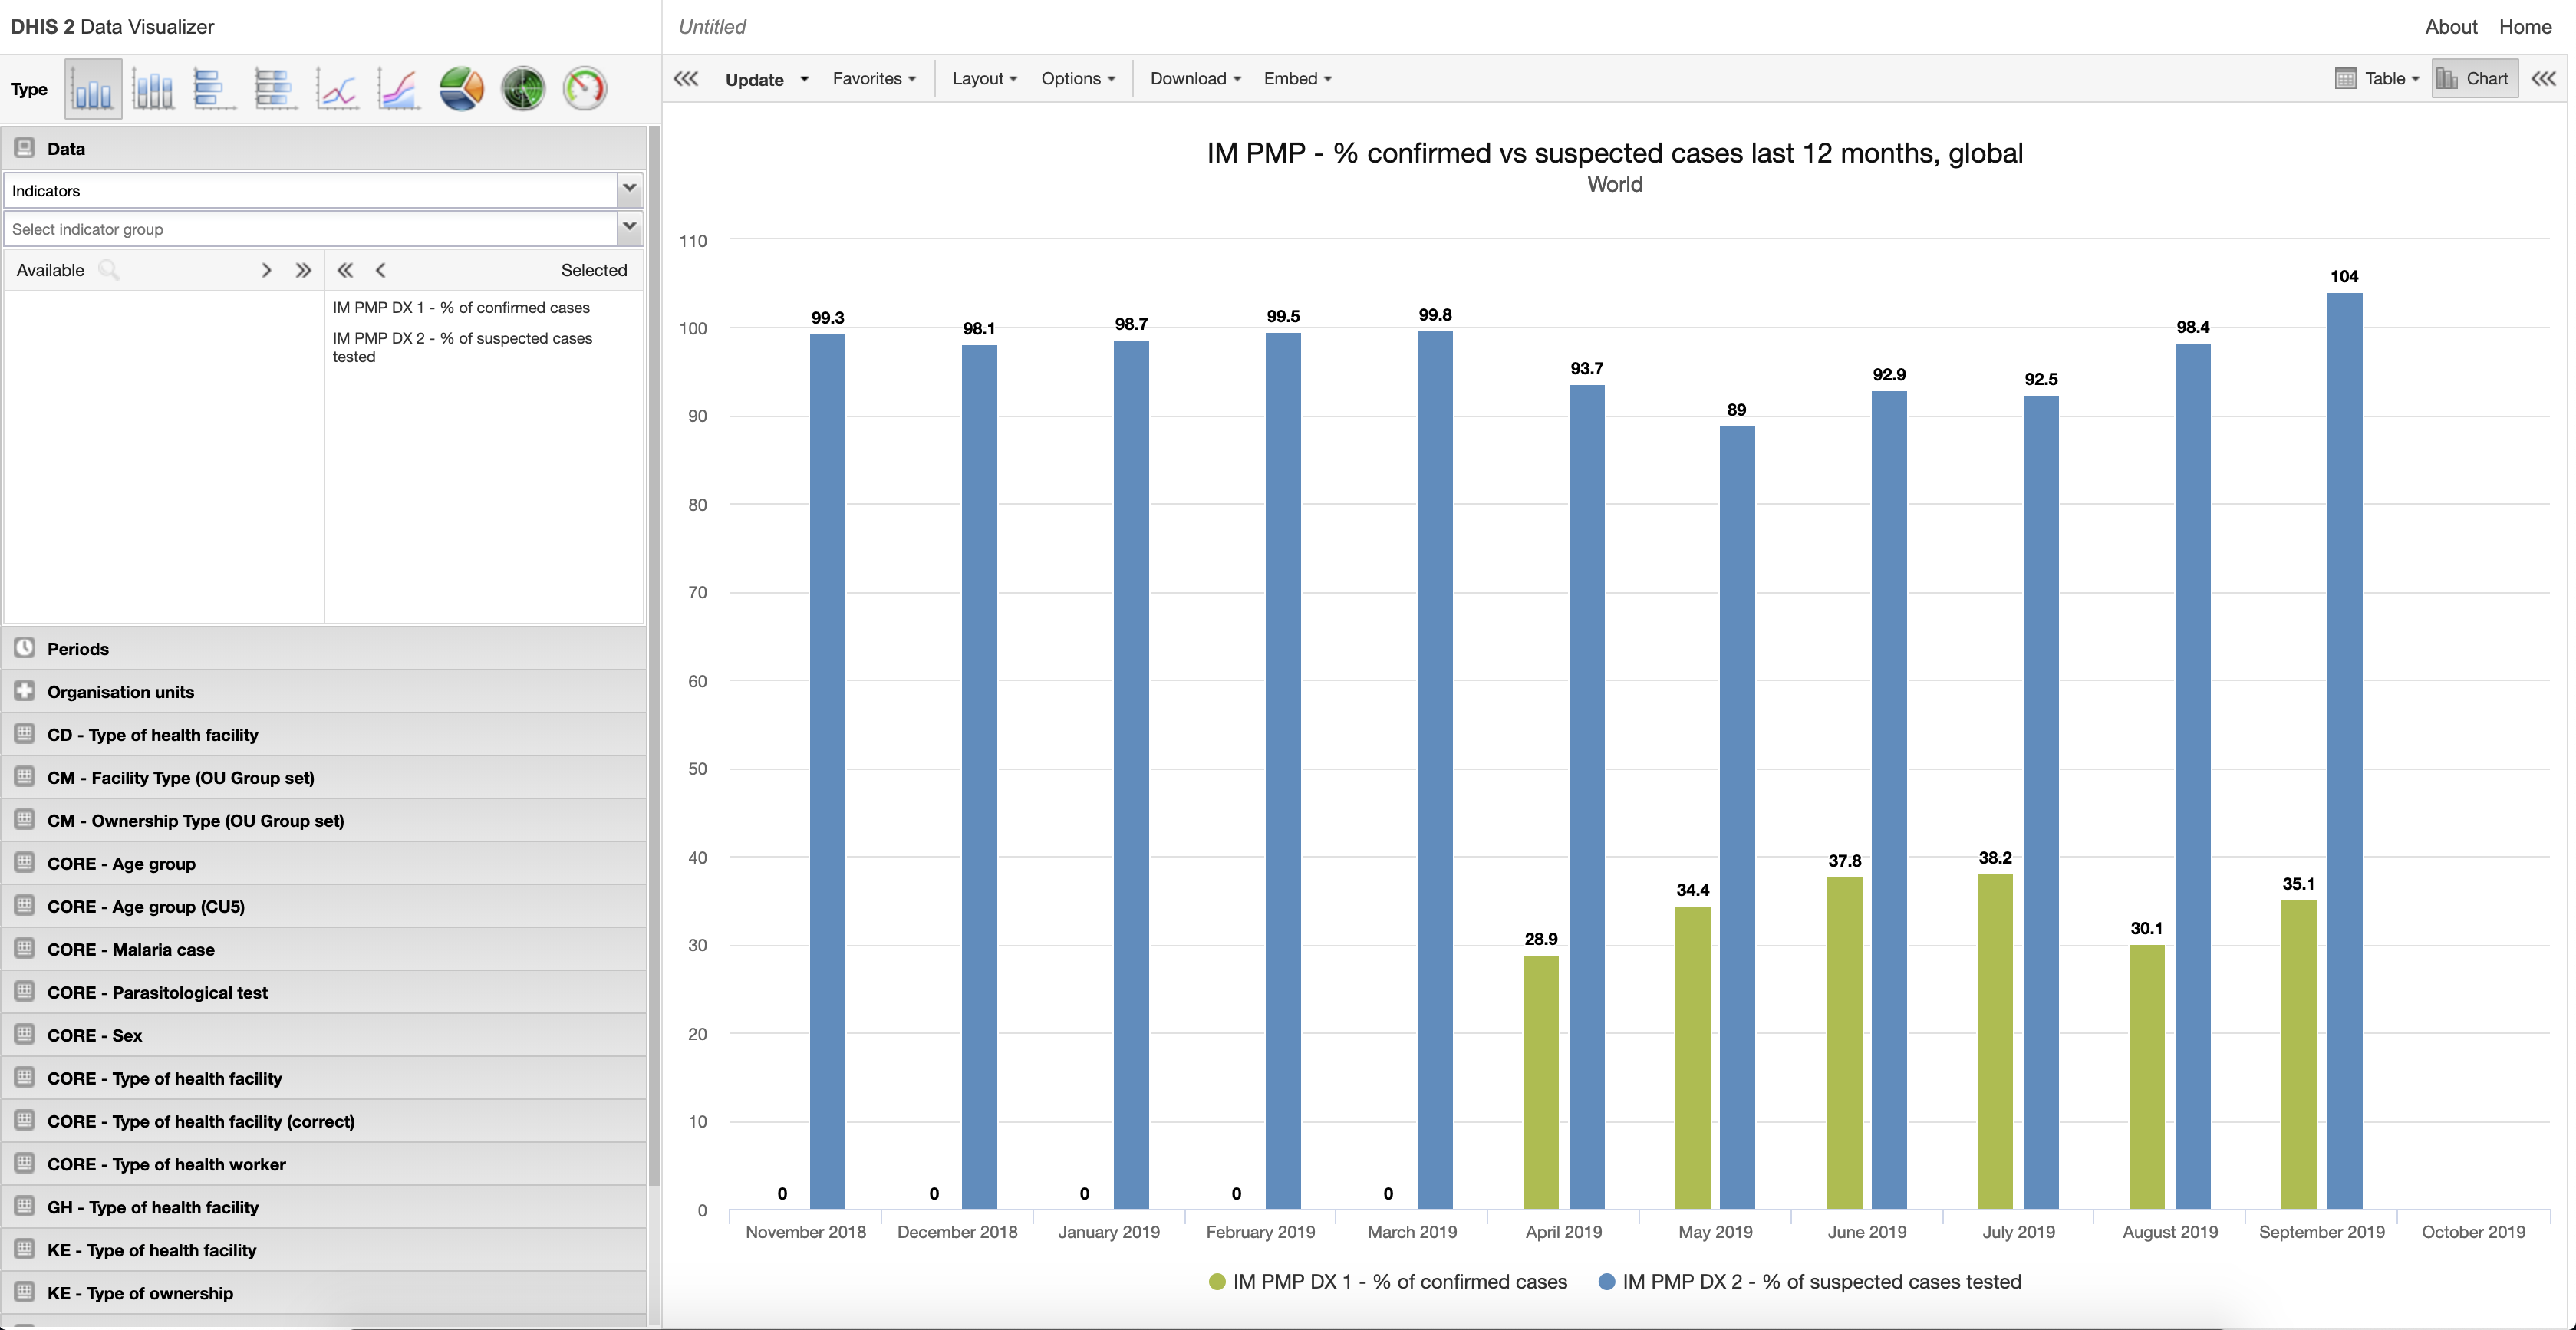
\includegraphics[width=46.64in]{./images/visualizer2} \caption{A bar chart generated by Data Visualizer App}\label{fig:visualizer2}
  \end{figure}
\end{enumerate}

By default, \texttt{open\ this\ table\ as\ chart} will attempt to visualize the table in a bar chart. We can switch to this chart to different types by selecting the \texttt{type}. Ensure you choose the appropriate type.

We'll stick to this as it is the most appropriate for this case. It shows the comparison.

\begin{quote}
Save your chart as \texttt{IM\ PMP\ -\ \%\ confirmed\ vs\ suspected\ cases\ last\ 12\ months,\ global}
\end{quote}

\hypertarget{map}{%
\subsection{Maps}\label{map}}

The Maps app allows you to set thematic layers of the areas and points, view facilities based on classifications, and visualize catchment areas for the geographical distribution of the IM data elements and indicators.

Example: Malaria Confirmed Cases in the last 3 months by region, Ghana.

\begin{figure}
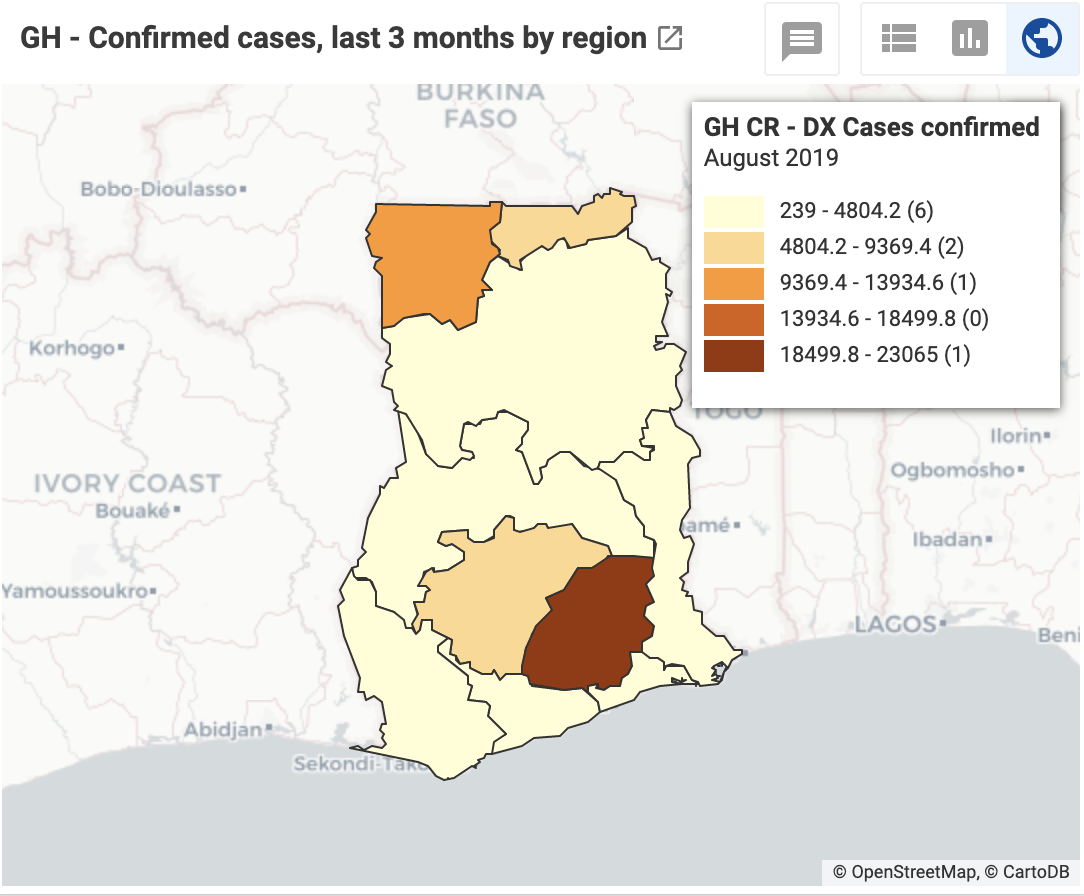
\includegraphics[width=15.06in]{./images/maps2} \caption{Malaria Confirmed Cases last 3 months by Region, Ghana}\label{fig:maps2}
\end{figure}

To create the map:

\begin{enumerate}
\def\labelenumi{\arabic{enumi}.}
\item
  Navigate to the \texttt{Maps} app

  \begin{figure}
  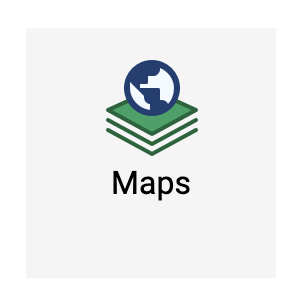
\includegraphics[width=4.25in]{./images/map} \caption{The Maps App}\label{fig:map}
  \end{figure}
\item
  Click the icon \texttt{Maps} to launch the app
\item
  Add a \texttt{thematic\ layer}

  \begin{figure}
  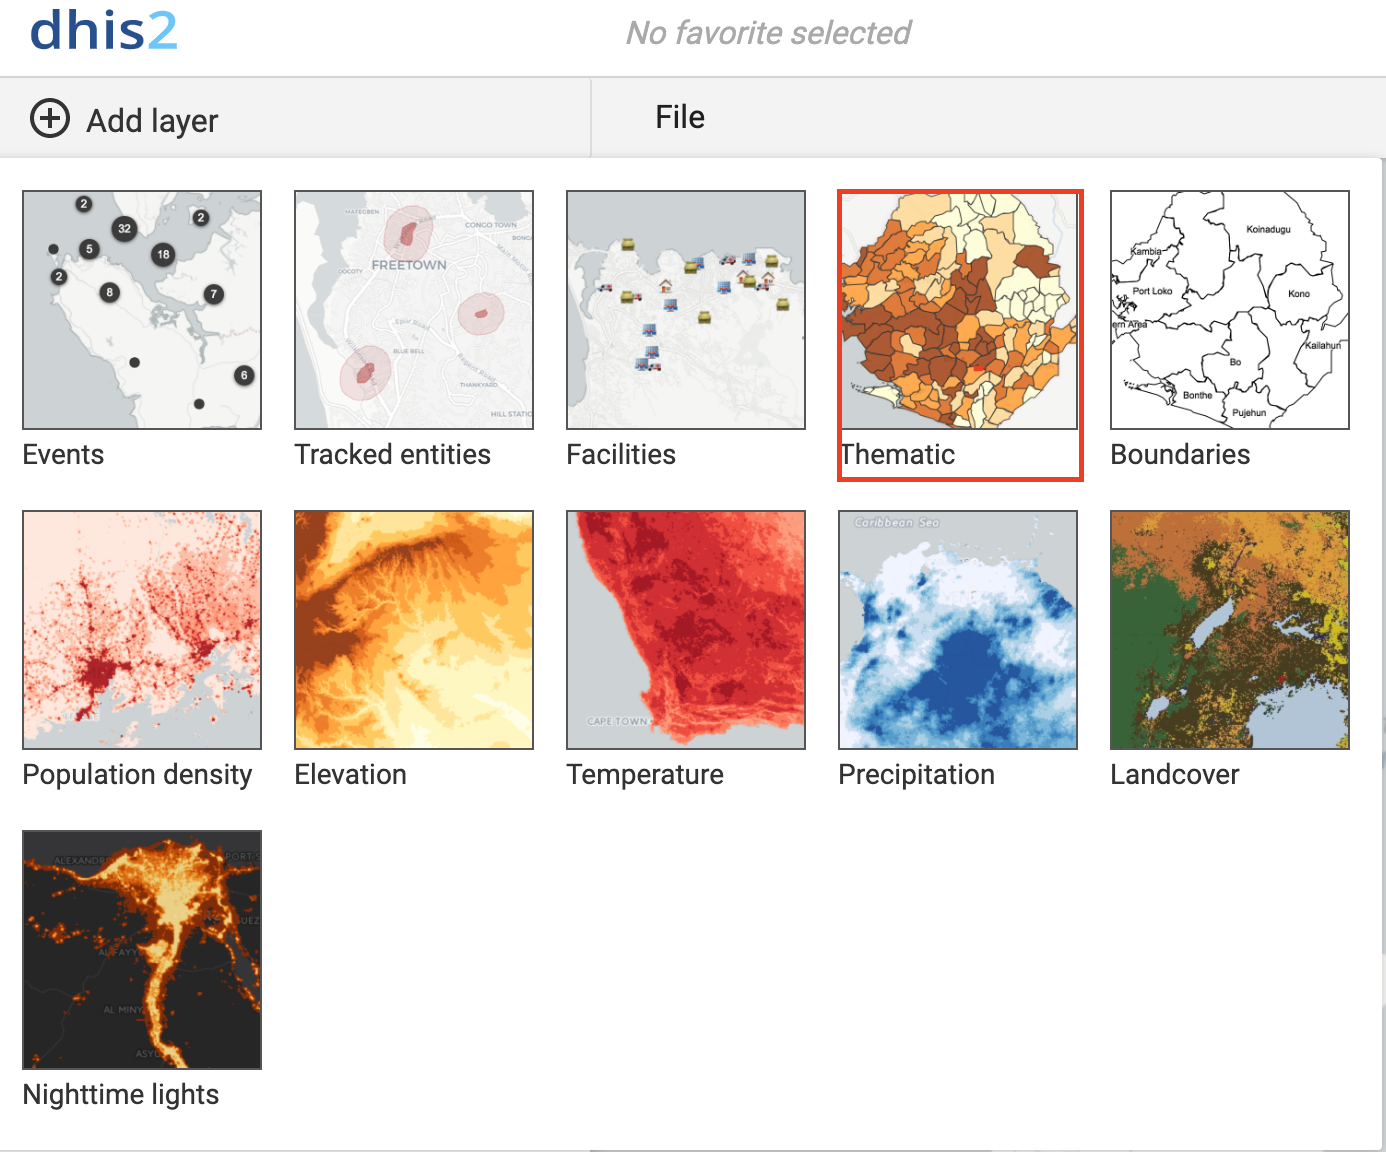
\includegraphics[width=19.25in]{./images/maps1} \caption{Select thematic layer}\label{fig:maps1}
  \end{figure}
\item
  Follow the steps to select the dimensions; What, when and where

  \begin{figure}
  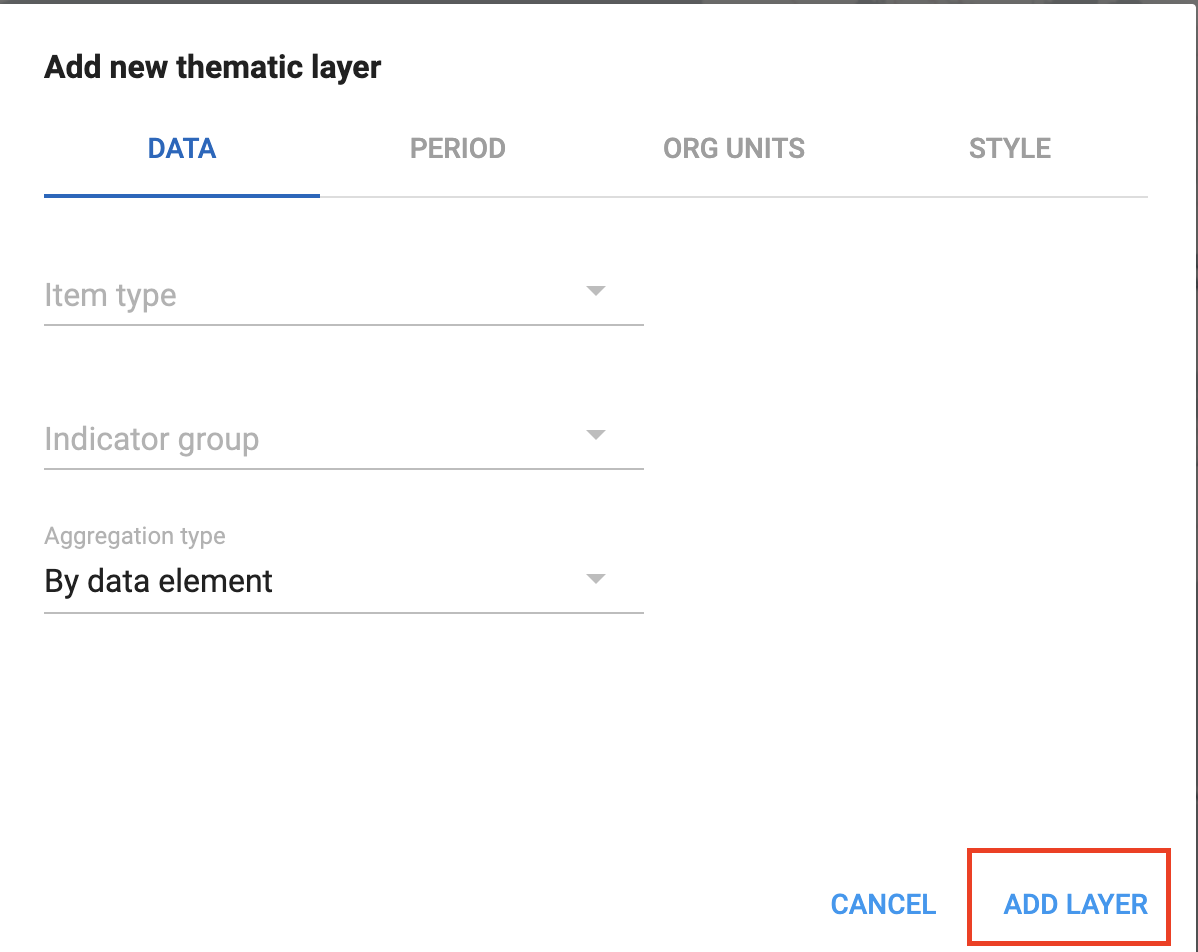
\includegraphics[width=16.64in]{./images/maps} \caption{Steps to select the dimensions; What, when and where}\label{fig:maps}
  \end{figure}
\item
  Update the layer
\end{enumerate}

\hypertarget{best-practices-tips-tricks-1}{%
\subsubsection{Best practices, tips \& tricks}\label{best-practices-tips-tricks-1}}

\begin{enumerate}
\def\labelenumi{\arabic{enumi}.}
\tightlist
\item
  Try not to put many overlapping layers on a map that will be difficult to interpret,
\item
  Use different color schemes when displaying multiple layers on a map,
\item
  The ordering of the layers is 1: Top Most Layer - 4: Bottom Most Layer. Add thematic layers to the map with this in mind.
\end{enumerate}

\hypertarget{data-presentation}{%
\section{Data Presentation}\label{data-presentation}}

Once the IM data elements and PMP indicators are analyzed, processed, and you've come up with different information products, the next big thing is how this information is used in the routine monitoring of the project.

Data use is an art by itself. Some several guides and structures attempt to promote data use. For the IM Data Hub, we promote the use of the Data-to-Action (D2A) frameworks as a tool to strenghten data use for decision-making.

\hypertarget{data}{%
\chapter{IM Data Specification}\label{data}}

\hypertarget{introduction-1}{%
\section{Introduction}\label{introduction-1}}

The IM data is specified through the use indicators. Indicators consist of a numerator, denominator, and a type of count. The numerator and denominator are data elements, and the count specifies the applied operation. Counts can be a percentage, a number, or a ratio.

In this chapter, we are going to explore the IM indicators and how they are constructed in the Data Hub.

We'll start by a short introduction to data elements and how they form the base/source of the IM indicators. We'll then explore the different counts and wind up by showing you all the IM indicators.

\hypertarget{data-elements-1}{%
\section{Data Elements}\label{data-elements-1}}

Data elements form the base of IM indicators. As we mentioned in the previous chapter, they define how IM data are collected and stored in the IM Data Hub.

IM Data hub consists of:
Global data elements - are shared across a number of countries,
Country specific data elements - used by specific country data sets.

IM data elements are grouped into data elements groups by country and programs for easy access from the Analytics apps in DHIS2 (Pivot Table, Data Visualizer and Maps).

The data elements have the following key fields:

\begin{enumerate}
\def\labelenumi{\arabic{enumi}.}
\tightlist
\item
  \texttt{uid,\ name,\ shortName,\ and\ code} for uniquely identifying the data element in the IM Data Hub,
\item
  \texttt{description} to document more information about the data point,
\item
  \texttt{formName} that appears on the data entry form (in our case, data sets),
\item
  \texttt{domainType} that specifies the data model - aggregate or tracker (in our case, aggregate),
\item
  \texttt{aggregationType} defines how data is stored in the IM Data Hub.
\end{enumerate}

\hypertarget{counts}{%
\section{Counts}\label{counts}}

Counts define the operation applied to the IM indicators calculations.

There are four main types of operations:

\begin{enumerate}
\def\labelenumi{\arabic{enumi}.}
\tightlist
\item
  \texttt{1\ -\ Atomic\ (number)} - absolute numbers
\item
  \texttt{1\ -\ Ratio} - a fraction of the numerator and denominator
\item
  \texttt{100\ -\ percent} - a ratio multiplied by 100 percent
\item
  \texttt{1000\ -\ per\ thousand} - a ratio multiplied by 1000
\end{enumerate}

\hypertarget{ind}{%
\section{Indicators}\label{ind}}

Remember that an indicator has a numerator, a denominator and a count. In this section, you will notice that similar to data elements, indicators also have the uid, short name and code to uniquely identifying them in the IM Data Hub.

The IM PMP indicators are grouped into two types:

Global IM PMP indicators - computes PMP data for global access,
Country Specific PMP indicators - computes PMP data for country access.

We present to you a list of all the IM indicators in section \ref{global-ind}

\hypertarget{global-ind}{%
\subsection{Global IM PMP indicators}\label{global-ind}}

code

name

shortName

numerator

denominator

count

DX indicators

IM PMP DX 01

IM PMP DX 01 - Percentage of confirmed malaria cases

IM PMP DX 01 - \% of confirmed cases

Number of cases confirmed as malaria by a parasitological test (RDT or microscopy)id : \#\{UFGPsP6p9mm\} + \#\{cZuXXzQuEL6\} + \#\{EIkFrm5x8Sf\} + \#\{gIFzQQKCMjb\}

Total number of suspected malaria cases who received a parasitological testid : \#\{N6j1f9LZiLf\} + \#\{zsUZQV4CAd6\} + \#\{BAZd7D3zQHN\} + \#\{Rf40G3xMCqI\}

100 - Per Cent

IM PMP DX 01 NP

IM PMP DX 01 - Percentage of confirmed malaria cases (NP)

IM PMP DX 01 - \% of confirmed cases (NP)

Number of cases confirmed as malaria by a parasitological test (RDT or microscopy)id : \#\{sZoMIJ8KFiw\}

Total number of suspected malaria cases who received a parasitological testid : \#\{uZWRcBbXVO5\}

100 - Per Cent

IM PMP DX 01 P

IM PMP DX 01 - Percentage of confirmed malaria cases (P)

IM PMP DX 01 - \% of confirmed cases (P)

Number of cases confirmed as malaria by a parasitological test (RDT or microscopy)id : \#\{CrV5hkFVvdH\}

Total number of suspected malaria cases who received a parasitological testid : \#\{hoGKdACnBUs\}

100 - Per Cent

IM PMP DX 02

IM PMP DX 02 - Percentage of patients with suspected malaria who received a parasitological test

IM PMP DX 02 - \% of suspected cases tested

Number of suspected malaria cases who received a parasitological testid : \#\{N6j1f9LZiLf\} + \#\{BAZd7D3zQHN\} + \#\{zsUZQV4CAd6\} + \#\{Rf40G3xMCqI\}

Total number of suspected cases of malariaid : \#\{eHWYhy8vO8q\} + \#\{euw633Z8zIo\} + \#\{m2CdUYVjGe5\} + \#\{LMMJ97M5sVl\}

100 - Per Cent

IM PMP DX 02 NP

IM PMP DX 02 - Percentage of patients with suspected malaria who received a parasitological test (NP)

IM PMP DX 02 - \% of suspected cases tested (NP)

Number of suspected malaria cases who received a parasitological testid : \#\{uZWRcBbXVO5\}

Total number of suspected cases of malariaid : \#\{DGZDsRtmqL7\}

100 - Per Cent

IM PMP DX 02 P

IM PMP DX 02- Percentage of patients with suspected malaria who received a parasitological test (P)

IM PMP DX 02 - \% of suspected cases tested (P)

Number of suspected malaria cases who received a parasitological testid : \#\{hoGKdACnBUs\}

Total number of suspected cases of malariaid : \#\{erW9vdRJVSE\}

100 - Per Cent

IM PMP DX 03

IM PMP DX 03 - Percentage of health workers demonstrating competence in correctly classifying cases as not malaria, uncomplicated malaria, and severe malaria

IM PMP DX 03 - \% of HWs able to classify cases

Number of health workers who demonstrate correct procedures for correctly classifying cases according to global standardsid : \#\{Grnm6jdzAJI\} + \#\{t1vdNH0vIE2\} + \#\{cVUt7HK83ag\} + \#\{vXZ2RDwuyzA\}

Total number of health workers targeted during the reporting periodid : \#\{SZKdCBFJd96\} + \#\{blbz5pmEqoF\} + \#\{pgsaevmKtbM\} + \#\{ytbfyxZr1Ya\}

100 - Per Cent

IM PMP DX 04

IM PMP DX 04 - Percentage of health workers demonstrating competence in malaria RDTs

IM PMP DX 04 - \% of HWs competent in RDTs

Number of health workers who score 90\% or greater in preparation and reading of RDTs during the training post-testid : \#\{Mfkn1qCEQEL\} + \#\{TDBa7IcPJAN\} + \#\{eEWSWmY9ghg\} + \#\{s5Ys2ABMGgE\}

Total number of health workers who completed a post-test during a trainingid : \#\{bWQoETmKYEh\} + \#\{rSn9x2JQPJe\} + \#\{soWdw75XP5d\} + \#\{QniAsU4SnZr\}

100 - Per Cent

IM PMP DX 05

IM PMP DX 05 - Percentage of health workers demonstrating competence in malaria microscopy

IM PMP DX 05 - \% of HWs competent in microscopy

Number of health workers who score 90\% or greater in slide preparation and parasite detection during the training post-testid : \#\{mYlff5bXuZB\} + \#\{x7CZVlQSaE6\} + \#\{JygaBsHMOQ0\} + \#\{jf8nKluaF2h\}

Total number of health workers who completed a post-test during a trainingid : \#\{f959MLmYSiX\} + \#\{VdW9y4M8WAK\} + \#\{XenaBO47ky4\} + \#\{om6201JM4BF\}

100 - Per Cent

PMP DX 06

IM PMP DX 06 - Percentage of targeted facilities that meet standards (including appropriate materials, documentation, and qualified staff) for quality diagnosis of malaria

IM PMP DX 06 - \% of facilities with quality DX

Number of targeted facilities that meet 90\% of greater on facility checklists for diagnosis during supervisory visitsid : \#\{DTdMcXDeHFj\} + \#\{Gj8mqX5twDU\} + \#\{VQT4EOtPiwC\} + \#\{uykAN5XlXKK\} + \#\{TLuXiPIlTDu\} + \#\{lYVEbBi1otu\}

Total number of targeted facilities who received a supervisory visit during the reporting periodid : \#\{aRCKf2dnCpw\} + \#\{oVIXBtQccHN\} + \#\{teWZva5EkPM\}

100 - Per Cent

PMP DX 07 MC

IM PMP DX 07 - Percentage of targeted facilities with at least one provider trained in malaria diagnosis (microscopy)

IM PMP DX 07 - \% of facilities trained (microsc)

0id : \#\{JJ9yeyBfn5V\} + \#\{RjcTcWjtJEh\}

0id : \#\{VX2UY9s7UTQ\}

100 - Per Cent

PMP DX 07 RDT

IM PMP DX 07 - Percentage of targeted facilities with at least one provider trained in malaria diagnosis (RDT)

IM PMP DX 07 - \% of facilities trained on RDT

Number of targeted facilities with one or more health workers trained in malaria diagnosisid : \#\{GFDsEzfZdjr\} + \#\{N6oAUOjFBF0\} + \#\{g1KI3UhtDoJ\}

Total number of targeted facilitiesid : \#\{VX2UY9s7UTQ\} + \#\{YpbUdDBZjlA\} + \#\{tWSq7bigbmf\}

100 - Per Cent

PMP DX 08 MC

IM PMP DX 08 - Percentage of targeted health workers trained in malaria laboratory diagnostics (microscopy)

IM PMP DX 08 - \% of HWs trained on (microscopy)

Number of health workers who complete the training course in malaria laboratory diagnostics (microscopy)id : \#\{f959MLmYSiX\} + \#\{GCSv8Ni4KhE\} + \#\{VdW9y4M8WAK\} + \#\{XenaBO47ky4\}

Total number of targeted health workersid : \#\{opuW5lGx2Cc\} + \#\{CX09R9Mdsj9\} + \#\{VcPN46GIkwA\} + \#\{a2RpS8B1eCM\}

100 - Per Cent

PMP DX 08 RDT

IM PMP DX 08 - Percentage of targeted health workers trained in malaria laboratory diagnostics (RDT)

IM PMP DX 08 - \% of HWs trained on RDT

Number of health workers who complete the training course in malaria laboratory diagnosticsid : \#\{bWQoETmKYEh\} + \#\{rSn9x2JQPJe\} + \#\{QniAsU4SnZr\} + \#\{soWdw75XP5d\}

Total number of targeted health workersid : \#\{opuW5lGx2Cc\} + \#\{a2RpS8B1eCM\} + \#\{CX09R9Mdsj9\} + \#\{VcPN46GIkwA\}

100 - Per Cent

PMP DX 09 MC

IM PMP DX 09 - Percentage of targeted supervisors trained in supervision of malaria diagnostics (microscopy)

IM PMP DX 09 - \% of SUPVs trained on microscopy

Number of supervisors trained in supervision of malaria diagnosticsid : \#\{RnEg1HPF7IR\} + \#\{hbEgIBy1bIf\} + \#\{zlWYhVAouup\} + \#\{PgAauebV15e\} + \#\{vg88HQNpSXz\}

Total number of targeted supervisorsid : \#\{cGXuIzDaAEP\} + \#\{MFpS8w5h9XS\} + \#\{pVyN8ZZT7TA\} + \#\{aZpDapygzg1\} + \#\{O8ilhnRgkRW\}

100 - Per Cent

PMP DX 09 RDT

IM PMP DX 09 - Percentage of targeted supervisors trained in supervision of malaria diagnostics (RDT)

IM PMP DX 09 - \% of SUPVs trained on RDT

Number of supervisors trained in supervision of malaria diagnosticsid : \#\{rvPl8m8kted\} + \#\{sRz3zlhaJrH\} + \#\{jZmH2n22eJf\} + \#\{oFiMCwBOYLU\}

Total number of targeted supervisorsid : \#\{cGXuIzDaAEP\} + \#\{MFpS8w5h9XS\} + \#\{pVyN8ZZT7TA\} + \#\{aZpDapygzg1\}

100 - Per Cent

PMP DX 10

IM PMP DX 10 - Percentage of targeted countries with national malaria diagnostic supervision tools that adhere to global standards

IM PMP DX 10 - \% of countries with DX tools

Number of targeted countries whose national malaria diagnostic supervision tools adhere to global standardsid : \#\{y2aPasQa1gl\}

Total number of targeted countriesid : \#\{y2aPasQa1gl\} \textgreater{}= 0

100 - Per Cent

PMP DX 11

IM PMP DX 11 - Percentage of targeted countries with national guidelines for malaria diagnosis that meet global standards

IM PMP DX 11 - \% of countries with DX guidelines

Number of targeted countries with national guidelines for malaria diagnosis that meet global standards/id : \#\{MUKvaz7q2CD\}

Total number of targeted countriesid : \#\{MUKvaz7q2CD\} \textgreater{}= 0

100 - Per Cent

MIP indicators

PMP MIP 25

IM PMP MIP 25 - Percentage of pregnant women who received an ITN during routine ANC

IM PMP MIP 25 - \% of pregnant women received ITN

Number of pregnant women who received an insecticide-treated net (ITN) during routine antenatal care (ANC)id : \#\{p4bKkXlEOtC\} + \#\{jmLXEBQDZAy\} + \#\{mEuLOT08NfK\} + \#\{kZAWqatScJ9\}

Total number of pregnant women attending antenatal visits (Number of first ANC visits as proxy in most countries' RHIS)id : \#\{jNJNr4i82le\} + \#\{IGyPotenyO2\} + \#\{WdEGVnuWiDf\} + \#\{KBe7hShEYAK\}

100 - Per Cent

PMP MIP 26

IM PMP MIP 26 - Percentage of pregnant women who received three or more doses of IPTp

IM PMP MIP 26 - \% of pregnant women with IPTp \textgreater{}=3

Number of pregnant women who received three or more doses of IPTp (IPT3)id : \#\{IGhCODoV6YY\} + \#\{RS90YaqGgUN\} + \#\{lVRMHcwVnDf\} + \#\{CFaVHFhbS4v\}

Total number of pregnant women attending antenatal visits (Number of first ANC visits as proxy in most countries' RHIS)id : \#\{jNJNr4i82le\} + \#\{IGyPotenyO2\} + \#\{WdEGVnuWiDf\} + \#\{KBe7hShEYAK\}

100 - Per Cent

PMP MIP 27

IM PMP MIP 27 - Percentage of pregnant women who received two doses of IPTp

IM PMP MIP 27 - \% of pregnant women with IPTp = 2

Number of pregnant women who received two doses of IPTp (IPT2)id : \#\{Y73pLgWXfTh\} + \#\{LF9PqTGXhBc\} + \#\{inFlJdtBRGo\} + \#\{SZgN28ZELh9\}

Total number of pregnant women attending antenatal visits (Number of first ANC visits as proxy in most countries' RHIS)id : \#\{jNJNr4i82le\} + \#\{IGyPotenyO2\} + \#\{WdEGVnuWiDf\} + \#\{SZgN28ZELh9\}

100 - Per Cent

PMP MIP 28

IM PMP MIP 28 - Percentage of pregnant women who received one dose of IPTp

IM PMP MIP 28 - \% of pregnant women with IPTp = 1

Number of pregnant women who received one dose of IPTp (IPT1)id : \#\{i5xgliv1YDl\} + \#\{qk8A67ySRR0\} + \#\{jrvQeHC4vrr\} + \#\{uuWSsTIrVtU\}

Total number of pregnant women attending antenatal visits (Number of first ANC visits as proxy in most countries' RHIS)id : \#\{jNJNr4i82le\} + \#\{IGyPotenyO2\} + \#\{WdEGVnuWiDf\} + \#\{KBe7hShEYAK\}

100 - Per Cent

PMP MIP 29

IM PMP MIP 29 - Percentage of targeted health workers demonstrating competence in treatment of MiP

IM PMP MIP 29 - \% of HWs competent in MiP (TX)

Number of health workers who score a pass mark on supervisory or quality improvement checklists measuring case management of MiPid : \#\{vKOVZ3Jckex\} + \#\{AkJUjEErkX5\} + \#\{RJVSWuXI87o\} + \#\{S2sRLkbN81y\}

Total number of targeted health workers who received a supervisory visit during the reporting periodid : \#\{t7LA2WZducS\} + \#\{yOXzK6ElVJr\} + \#\{gnjJPPJNSJF\} + \#\{fJIele1NEHo\}

100 - Per Cent

PMP MIP 30

IM PMP MIP 30 - Percentage of targeted health workers demonstrating competence in prevention of MiP

IM PMP MIP 30 - \% of HWs competent in MiP (PREV)

Number of health workers who score a pass mark on supervisory or quality improvement checklists measuring IPTp and counselling for MiPid : \#\{aOenVQmDtkc\}

Total number of targeted health workers who received a supervisory visit during the reporting periodid : \#\{fpDelOtHjG4\}

100 - Per Cent

PMP MIP 31

IM PMP MIP 31 - Percentage of health workers trained in IPTp

IM PMP MIP 31 - \% of HWs trained on IPTp

Number of health workers who complete the training course on IPTpid : \#\{yQ11Q5pQ2lx\} + \#\{CxioZ7hV8e9\} + \#\{eEITioVuAGg\} + \#\{jKtX2TrReqh\}

Total number of targeted health workersid : \#\{yoNR9Ct37gT\} + \#\{FVF9sYgBAH2\} + \#\{wHuGUXeSGM8\} + \#\{bf7z94n1SLP\}

100 - Per Cent

PMP MIP 32

IM PMP MIP 32 - Percentage of targeted countries with national guidelines for prevention and treatment of MiP that meet global standards

IM PMP MIP 32 - \% of countries with MiP guides

Number of targeted countries with national guidelines for prevention and treatment of MiP that meet global standardsid : \#\{C0UniRKgGAG\}

Total number of targeted countriesid : \#\{C0UniRKgGAG\}\textgreater{}=0

100 - Per Cent

PMP MIP 33

IM PMP MIP 33 - Functional active RMNCH/MiP/ANC/community health Working Group

IM PMP MIP 33 - Active HWGs

Functional/active malaria/MiP/ANC/community health or RMNCH Working Group with a MiP lens that meets periodicallyid : \#\{wHtxPnCGqBV\}

Functional/active malaria/MiP/ANC/community health or RMNCH Working Group with a MiP lens that meets periodicallyid : \#\{wHtxPnCGqBV\}\textgreater{}=0

1 - Atomic (number)

SMC indicators

PMP SMC 34

IM PMP SMC 34 - Percentage of targeted children who receive all 4 doses of SMC in a round in intervention area (or all 3 per national guidance where only 3 doses are indicated)

IM PMP SMC 34 - \% of children received 4 doses

Number of targeted children receiving all recommended SMC doses during a campaign, in the intervention areaid : \#\{ioU1w8yCIWv\}

Number of children in target age range in the intervention areaid : \#\{jAD6Dh7z1d1\}

100 - Per Cent

PMP SMC 35

IM PMP SMC 35 - Percentage of targeted children who receive a dose of SMC in intervention area

IM PMP SMC 35 - \% of children dosed

Number of targeted children receiving a dose of SMC in the intervention areaid : \#\{cOBjDRbvsyW\}

Number of children in target age range in the intervention areaid : \#\{wr0GInmvDcB\}

100 - Per Cent

PMP SMC 36

IM PMP SMC 36 - Percentage of targeted children who receive a dose of SMC in the first cycle

IM PMP SMC 36 - \% of children dosed (cy. 1)

Number of targeted children who received a dose of SMC during the first cycleid : \#\{HaSIpoMB2ub\}

Number of children in target age range in the intervention areaid : \#\{pW2ZZhtd9Lz\}

100 - Per Cent

PMP SMC 37

IM PMP SMC 37 - Percentage of targeted children who receive a dose of SMC in the second cycle

IM PMP SMC 37 - \% of children dosed (cy. 2)

Number of targeted children who received a dose of SMC during the second cycleid : \#\{wot02J4aRZm\}

Number of children in target age range in the intervention areaid : \#\{AiA5kpzCOVw\}

100 - Per Cent

PMP SMC 38

IM PMP SMC 38 - Percentage of targeted children who receive a dose of SMC in the third cycle

IM PMP SMC 38 - \% of children dosed (cy. 3)

Number of targeted children who received a dose of SMC during the third cycleid : \#\{ZCibgANrNQq\}

Number of children in target age range in the intervention areaid : \#\{Q0hsAMcsvkm\}

100 - Per Cent

PMP SMC 39

IM PMP SMC 39 - Percentage of targeted children who receive a dose of SMC in the fourth cycle

IM PMP SMC 39 - \% of children dosed (cy. 4)

Number of targeted children who received a dose of SMC during the fourth cycleid : \#\{Q71hAveCSGo\}

Number of children in target age range in the intervention areaid : \#\{InNkmkUawo7\}

100 - Per Cent

PMP SMC 40

IM PMP SMC 40 - Percentage of health workers trained to deliver SMC according to national guidelines

IM PMP SMC 40 - \% of HWs trained on SMC

Number of health workers who complete the training course on delivering SMCid : \#\{y6qGAzE5DRa\}

Total number of targeted health workersid : \#\{nE14FEYzkVX\}

100 - Per Cent

PMP SMC 41

IM PMP SMC 41 - Percentage of targeted countries with annual SMC implementation plans

IM PMP SMC 41 - \% of countries with ANN SMC plans

Number of countries with annual operational SMC implementation plansid : \#\{hBYYaPLEFFf\}

Total number of targeted countries anticipated to have plansid : \#\{gN3w6Jx7q5h\}

100 - Per Cent

TL indicators

PMP TL 42

IM PMP TL 42 - Contribution to national, regional or global guidance/policy documents related to malaria (including RH)

IM PMP TL 42 - Contribution

Contribution to national, regional guidance/policy documents or related to malaria (including RH)id : \#\{tJXmW64MUxf\}

Contribution to national, regional guidance/policy documents or related to malaria (including RH)id : 1

1 - Atomic (number)

PMP TL 43

IM PMP TL 43 - Number of program activity outputs disseminated to the global health community

IM PMP TL 43 - Outputs to GH community

By type of output (activity reports, operational research/evaluation reports, technical briefs, learning briefs, synthesis brief, discussion brief, infographic, case studies, peer-reviewed publications, webinars, oral/poster presentations, blog posts, short video clips, photos) By dissemination channelid : \#\{P4YDP2FNh3X\}

By type of output (activity reports, operational research/evaluation reports, technical briefs, learning briefs, synthesis brief, discussion brief, infographic, case studies, peer-reviewed publications, webinars, oral/poster presentations, blog posts, short video clips, photos) By dissemination channelid : 1

1 - Atomic (number)

PMP TL 44

IM PMP TL 44 - Participation in targeted national, regional or global level Working group(s) and/or taskforce(s)

IM PMP TL 44 - Participation in TWGs.

Participation in national, regional or global working group(s) or taskforce(s) related to malaria (including RH)id : \#\{XxfoDreiw9Z\}

Participation in national, regional or global working group(s) or taskforce(s) related to malaria (including RH)id : 1

1 - Atomic (number)

TX indicators

PMP TX 12

IM PMP TX 12 - Percentage of children under 5 appropriately treated for fever according to iCCM or country algorithms by community health workers

IM PMP TX 12 - \% of CU5 fever treated

Number of children under 5 correctly treated for malaria fever by community health workerid : \#\{sYGiQi29bny\} + \#\{sHbqsn1y9zL\}

Number of CU5 presented to CHWs with feverid : \#\{jQCXu21pwiA\} + \#\{pGLrWpOTB1m\}

100 - Per Cent

PMP TX 13

IM PMP TX 13 - Percentage of confirmed severe malaria cases that were appropriately managed according to national guidelines

IM PMP TX 13 - \% of confirmed severe cases

Number of confirmed severe malaria cases that were appropriately managed according to national guidelinesid : \#\{WY24SnaT4l7\}

Number of severe malaria cases reviewedid : \#\{WY24SnaT4l7\}

100 - Per Cent

PMP TX 13 NP

IM PMP TX 13 - Percentage of confirmed severe malaria cases that were appropriately managed according to national guidelines (NP)

IM PMP TX 13 - \% of confirmed severe cases (NP)

Number of confirmed severe malaria cases that were appropriately managed according to national guidelines (NP)id : \#\{W6NdGzWJurN\}

Number of severe malaria cases reviewed (NP)id : \#\{W6NdGzWJurN\}

100 - Per Cent

PMP TX 13 P

IM PMP TX 13 - Percentage of confirmed severe malaria cases that were appropriately managed according to national guidelines (P)

IM PMP TX 13 - \% of confirmed severe cases (P)

Number of confirmed severe malaria cases that were appropriately managed according to national guidelines (P)id : \#\{h5toMEwrcCi\}

Number of severe malaria cases reviewed (P)id : \#\{h5toMEwrcCi\}

100 - Per Cent

PMP TX 14

IM PMP TX 14 - Percentage of uncomplicated malaria cases that received first-line antimalarial treatment according to national guidelines

IM PMP TX 14 - \% of uncomplicated cases

Number of reported uncomplicated malaria cases that receive the appropriate first-line antimalarial treatmentid : \#\{Aj2LczZnc35\} + \#\{JLxVyp3qGve\} + \#\{V6CvG07Copy\} + \#\{i4BsFSVy41V\}

Total number of reported malaria cases during reporting periodid : \#\{UFGPsP6p9mm\} + \#\{PoyoVEewRIq\} + \#\{EIkFrm5x8Sf\} + \#\{cZuXXzQuEL6\} + \#\{gIFzQQKCMjb\} + \#\{y8geJquiy1f\} + \#\{E04lKfKFlKc\}

100 - Per Cent

PMP TX 14 NP

IM PMP TX 14 - Percentage of uncomplicated malaria cases that received first-line antimalarial treatment according to national guidelines (NP)

IM PMP TX 14 - \% of uncomplicated cases (NP)

Number of reported uncomplicated malaria cases that receive the appropriate first-line antimalarial treatment (NP)id : \#\{RYl937S07k0\} + \#\{n9YAgSwzX8J\} + \#\{Jz05wiLIOae\}

Total number of reported malaria cases during reporting periodid : \#\{sZoMIJ8KFiw\}+\#\{RnZK9U6WoAm\}+ \#\{WuWNNgy0A1Z\} + \#\{rKatBh8TmW2\} + \#\{KcMPvVefT1h\}

100 - Per Cent

PMP TX 14 P

IM PMP TX 14 - Percentage of uncomplicated malaria cases that received first-line antimalarial treatment according to national guidelines (P)

IM PMP TX 14 - \% of uncomplicated cases (P)

Number of reported uncomplicated malaria cases that receive the appropriate first-line antimalarial treatmentid : \#\{Ldvf3MSggqO\} + \#\{KZHiYuvgkMm\} + \#\{PfB1cg2ktB9\}

Total number of reported malaria cases during reporting periodid : \#\{CrV5hkFVvdH\} + \#\{qXQ0d9NKQtI\} + \#\{AmUi4XKbJ6X\} + \#\{HiIx2iQ8Wxy\} + \#\{YMiDfYBOpWk\} + \#\{RfziOIqzJCP\}

100 - Per Cent

PMP TX 14 P (CL)

IM PMP TX 14 - Percentage of uncomplicated malaria cases that received first-line antimalarial treatment according to national guidelines (P) (CL)

IM PMP TX 14 - \% of uncomplicated cases (P) (CL)

Number of reported uncomplicated malaria cases that receive the appropriate first-line antimalarial treatmentid : \#\{Ldvf3MSggqO\}

Total number of reported malaria cases during reporting periodid : \#\{CrV5hkFVvdH\} + \#\{qXQ0d9NKQtI\}

100 - Per Cent

PMP TX 15

IM PMP TX 15 - Percentage of targeted health workers demonstrating competence in management of severe malaria

IM PMP TX 15 - \% of HWs competent in severe cases

Number of health workers who score a pass mark on supervisory or quality improvement checklists measuring the diagnosis and management of severe malariaid : \#\{QYPXt95CyCY\} + \#\{es8NwgtSAsX\} + \#\{lomzmDp50ZG\} + \#\{Ct1pZ0T1x2R\}

Health workers assessed on diagnosis and management of severe malariaid : \#\{W4wiC7ioFKS\} + \#\{b3GBk3DB8ou\} + \#\{g0OQgJCDs0U\} + \#\{WNhkeZnc1XT\}

100 - Per Cent

PMP TX 16

IM PMP TX 16 - Percentage of targeted health workers demonstrating competence in management of uncomplicated malaria

IM PMP TX 16 - \% of HWs competent (uncomp cases)

Number of health workers who score a pass mark on supervisory or quality improvement checklists measuring the diagnosis and treatment of uncomplicated malariaid : \#\{gmsvdmKMmP1\} + \#\{l4uAwIXVrPp\} + \#\{HsD3L7BZa5T\} + \#\{umfGv9oznIa\}

Health workers assessed on diagnosis and management of uncomplicated malariaid : \#\{HcmlwDCmBSZ\} + \#\{uNnp6IHODyP\} + \#\{GtohCrGevVV\} + \#\{Wq1oBD43sCc\}

100 - Per Cent

PMP TX 17

IM PMP TX 17 - Percentage of targeted health workers demonstrating compliance to treatment with WHO guidelines for cases with positive malaria test results

IM PMP TX 17 - \% of HWs adhered (+ve cases)

Number of health workers who comply to treatment with a WHO-recommended antimalarial for cases with positive malaria test results during clinical assessment visits measured through direct observation during supervision visitsid : \#\{Do9KBfS22qD\} + \#\{eJSUmK8XCOw\} + \#\{wVlGTvl4xvH\} + \#\{E77z4UQBHJE\}

Health workers assessed on management of positive malaria casesid : \#\{Bli6iNQMtP5\} + \#\{w1gYh10blt1\} + \#\{ibu7rlMvF7s\} + \#\{YCsROGVIXGz\}

100 - Per Cent

PMP TX 18

IM PMP TX 18 - Percentage of health workers demonstrating adherence to negative test results according to global standards

IM PMP TX 18 - \% of HWs adhered (-ve cases)

Number of health workers demonstrating adherence to negative test results according to global standards measured through direct observation through supervision visitsid : \#\{jhcbf1Yfhr5\} + \#\{yChCRfBYBx2\} + \#\{u6hbx56NqZQ\} + \#\{Y0IgOx4kim8\}

Health workers assessed on management of negative malaria casesid : \#\{vskYxCrS9Hk\} + \#\{FORs5r9LYU3\} + \#\{oV5ypvYLOjj\} + \#\{WvrndytTbHq\}

100 - Per Cent

PMP TX 19

IM PMP TX 19 - Percentage of targeted facilities that meet standards (including appropriate materials, documentation, and qualified staff) for quality malaria case management

IM PMP TX 19 - \% of facilities with CM standards

Number of targeted facilities that meet 90\% or greater on facility checklists for quality case management during supervisory visitsid : \#\{Bjg3UQZTo7O\} + \#\{vsI12KXd1od\}

Total number of targeted facilities who received a supervisory visit during the reporting periodid : \#\{TpcOpmZBdLf\} + \#\{XY77QRYfFiA\}

100 - Per Cent

PMP TX 20

IM PMP TX 20 - Percentage of targeted health facilities regularly reporting routine malaria case data

IM PMP TX 20 - \% of facilities reporting cases

Number of health facilities reporting monthly routine malaria case load data on diagnosis and treatment within an agreed timescale at least 2 months in the past 3 monthsid : \#\{xV85TQT3GEj\}

Total number of target health facilities scheduled to report monthly routine malaria case load data during the reporting periodid : \#\{pDisUBYkiUY\}

100 - Per Cent

PMP TX 21

IM PMP TX 21 - Percentage of targeted health facilities that receive a supervisory visit

IM PMP TX 21 - \% of facilities with SUPV visits

Number of health facilities that receive a supervisory visit that covers malaria case management and/or malaria in pregnancy (MiP)id : \#\{TpcOpmZBdLf\}

Total number of health facilities targeted for supervision during the reporting periodid : \#\{RncgLNY0xwy\}

100 - Per Cent

PMP TX 22

IM PMP TX 22 - Percentage of health workers trained in management of severe malaria

IM PMP TX 22 - \% of HWs trained on severe malaria

Number of health workers who complete the training course on severe malaria case managementid : \#\{Ly61ha78oUu\}

Total number of health workers targetedid : \#\{DoyuoVEARPV\}

100 - Per Cent

PMP TX 23

IM PMP TX 23 - Percentage of targeted health workers trained according to national guidelines in malaria case management with ACTs

IM PMP TX 23 - \% of HWs trained on ACTs

Number of health workers who complete the national training course on malaria case management with ACTsid : \#\{wfxNAGkIedf\}

Total number of health workers targetedid : \#\{cqKHdgtfjID\}

100 - Per Cent

PMP TX 24

IM PMP TX 24 - Percentage of targeted countries with national guidelines for malaria treatment that meet global standards

IM PMP TX 24 - \% of countries with TX guidelines

Number of targeted countries with national guidelines for malaria treatment that meet global standardsid : \#\{YVLRuSGpePK\}

Total number of targeted countriesid : \#\{YVLRuSGpePK\}\textgreater{}0

100 - Per Cent

NA

IM PMP Tx 2 - Percentage of severe malaria cases appropriately managed

\% of severe malaria cases appropriately managed

Numid : \#\{km1lPVcORaY\}

Denid : \#\{W6NdGzWJurN\}

100 - Per Cent

NA

IM PMP Tx 3 - Percentage of uncomplicated malaria cases that received first-line antimalarial treatment according to national guidelines

\% of uncomplicated malaria cases managed

Numid : \#\{RYl937S07k0\}

Denid : \#\{oWhqaiv26dB\}

100 - Per Cent

\hypertarget{country-ind}{%
\subsection{Country IM PMP indicators}\label{country-ind}}

\hypertarget{kenya}{%
\subsubsection{Kenya}\label{kenya}}

code

name

shortName

numerator

denominator

count

DX indicators

NA

KE PMP 01 - DX Percentage of patients with suspected malaria who received a parasitological test

KE PMP 01 - DX \% tested suspected cases

Numid : \#\{Rf40G3xMCqI\}

Denid : \#\{m2CdUYVjGe5\}

100 - Per Cent

NA

KE PMP 02 - DX Percentage of health workers demonstrating competence in malaria RDTs

KE PMP 02 - DX \% HWs malaria RDTs

Numid : \#\{s5Ys2ABMGgE\}

Denid : \#\{soWdw75XP5d\}

100 - Per Cent

NA

KE PMP 03 - DX Percentage of HCWs demonstrating competence in malaria microscopy

KE PMP 03 - DX \% HWs malaria microscopy

Numid : \#\{x7CZVlQSaE6\}

Denid : \#\{VdW9y4M8WAK\}

100 - Per Cent

NA

KE PMP 04 - DX Percentage of targeted facilities that meet standards (including appropriate materials, documentation, and qualified staff) for quality diagnosis of malaria (microscopy)

KE PMP 04 - DX \% HFs malaria microscopy

Numid : \#\{uykAN5XlXKK\}

Denid : \#\{HDK9LRt5rDv\}

100 - Per Cent

NA

KE PMP 04 - DX Percentage of targeted facilities that meet standards (including appropriate materials, documentation, and qualified staff) for quality diagnosis of malaria (RDT)

KE PMP 04 - DX \% HFs malaria RDTs

Numid : \#\{TLuXiPIlTDu\}

Denid : \#\{HDK9LRt5rDv\}

100 - Per Cent

NA

KE PMP 05 - DX Percentage of HCWs demonstrating competence or knowledgeable in correctly classifying uncomplicated and severe malaria

KE PMP 05 - DX \% HWs classify cases correctly

Numid : \#\{cVUt7HK83ag\}

Denid : \#\{blbz5pmEqoF\}

100 - Per Cent

NA

KE PMP 06 - DX Percentage of targeted supervisors trained in supervision of malaria diagnostics (microscopy)

KE PMP 06 - DX \% supervisors trained (microscopy)

Numid : \#\{PgAauebV15e\}

Denid : \#\{pVyN8ZZT7TA\}

100 - Per Cent

NA

KE PMP 06 - DX Percentage of targeted supervisors trained in supervision of malaria diagnostics (RDT)

KE PMP 06 - DX \% supervisors trained (RDT)

Numid : \#\{jZmH2n22eJf\}

Denid : \#\{pVyN8ZZT7TA\}

100 - Per Cent

NA

KE PMP 07 - DX Percentage of targeted counties with recommended malaria diagnostic supervision tools

KE PMP 07 - DX \% counties w/malaria DX tools

Numid : \#\{zTF23dP6a65\}

Denid : R\{dfroFhEbqHJ.ACTUAL\_REPORTS\}

100 - Per Cent

NA

KE PMP 08 - DX DX Percentage of targeted health workers trained in malaria diagnostics (RDT)

KE PMP 08 - DX \% HWs trained (RDT)

Numid : \#\{soWdw75XP5d\}

Denid : \#\{a2RpS8B1eCM\}

100 - Per Cent

NA

KE PMP 08 - DX Percentage of targeted health workers trained in malaria diagnostics (microscopy)

KE PMP 08 - DX \% HWs trained (microscopy)

Numid : \#\{VdW9y4M8WAK\}

Denid : \#\{a2RpS8B1eCM\}

100 - Per Cent

NA

KE PMP 09 - DX Percentage of targeted facilities with at least one provider trained in RDT

KE PMP 09 - DX \% HFs with 1 provider trained (RDT)

Numid : \#\{g1KI3UhtDoJ\}

Denid : \#\{mZJOvYsr84U\}

100 - Per Cent

NA

KE PMP 10 - DX Percentage of targeted facilities with at least one provider trained in microscopy

KE PMP 10 - DX \% HFs with 1 provider trained (mic)

Numid : \#\{RjcTcWjtJEh\}

Denid : \#\{azuQmfnMNVU\}

100 - Per Cent

NA

KE PMP 11 - DX Percentage of targeted facilities with recommended guidelines/SOPs for malaria diagnosis

KE PMP 11 - DX \% HFs with SOPs

Numid : \#\{sjDRGLS9yjA\}

Denid : \#\{WrYkhf4k7pL\}

100 - Per Cent

TX indicators

NA

KE PMP 12 - TX Percentage of suspected cases confirmed +ve for malaria

KE PMP 12 - TX \% confirmed malaria cases

Numid : \#\{gIFzQQKCMjb\}

Denid : \#\{Rf40G3xMCqI\}

100 - Per Cent

NA

KE PMP 13 - TX Percentage of confirmed uncomplicated malaria cases that received first-line antimalarial treatment according to recommended national guidelines

KE PMP 13 - TX \% cases correctly treated

Numid : \#\{V6CvG07Copy\}

Denid : \#\{gIFzQQKCMjb\}

100 - Per Cent

NA

KE PMP 14 - TX Percentage of laboratory confirmed severe malaria cases treated according to recommended guidelines (the administration of a recommended antimalarial)

KE PMP 14 - TX \% severe cases correctly treated

Numid : \#\{dumrnf9ppLQ\}

Denid : \#\{T32qa5ftQkW\}

100 - Per Cent

NA

KE PMP 15 - TX Percentage of targeted HCWs demonstrating compliance to treatment according to national guidelines for cases with positive malaria test results

KE PMP 15 - TX \% HWs compliance positive cases

Numid : \#\{E77z4UQBHJE\}

Denid : \#\{YCsROGVIXGz\}

100 - Per Cent

NA

KE PMP 16 - TX Percentage of HCWs demonstrating adherence to negative test results according to recommended guidelines

KE PMP 16 - TX \% HWs compliance negative cases

Numid : \#\{Y0IgOx4kim8\}

Denid : \#\{oV5ypvYLOjj\}

100 - Per Cent

NA

KE PMP 17 - TX Percentage of targeted HCWs demonstrating competence in management of severe malaria according to national guidelines

KE PMP 17 - TX \% HWs competent severe cases

Numid : \#\{Ct1pZ0T1x2R\}

Denid : \#\{WNhkeZnc1XT\}

100 - Per Cent

NA

KE PMP 18 - TX Percentage of targeted HCWs demonstrating competence in management of uncomplicated malaria according to national guidelines

KE PMP 18 - TX \% HWs competent unc malaria

Numid : \#\{umfGv9oznIa\}

Denid : \#\{GtohCrGevVV\}

100 - Per Cent

NA

KE PMP 19 - TX Percentage of targeted facilities that meet global standards (including appropriate materials, documentation, and qualified staff) for quality malaria case management

KE PMP 19 - TX \% HFs compliant quality case mngt

Numid : \#\{Sigw3MWtZ5d\}

Denid : \#\{YZCHWOIahjV\}

100 - Per Cent

NA

KE PMP 20 - TX Percentage of admitting facilities with HCWs trained in management of severe malaria

KE PMP 20 - TX \% HFs provider trained (severe)

Numid : \#\{JVOBcq2tayS\}

Denid : \#\{A20vEAmjRAS\}

100 - Per Cent

NA

KE PMP 21 - TX Percentage of health workers trained on malaria case management

KE PMP 21 - TX \% HWs trained case mngt

Numid : \#\{Y2Wizwyg2Zt\}

Denid : \#\{HKwLM21EySC\}

100 - Per Cent

NA

KE PMP 22 - TX Percentage of targeted health facilities that receive a supervisory visit

KE PMP 22 - TX \% HFs supervised

Numid : \#\{egcmJ7NFPBG\}

Denid : \#\{WRP6ICberkf\}

100 - Per Cent

NA

KE PMP 23 - TX Percentage of targeted health facilities regularly reporting routine malaria case data

KE PMP 23 - TX \% HFs reporting on time

Numid : \#\{A6is0WZ7UVI\}+\#\{WUsfoJ01oa8\}

Denid : \#\{k0OSOd7UeDj\}+\#\{Jz08Pq3eoMi\}

100 - Per Cent

MIP indicators

NA

KE PMP 24 - MIP Percentage of pregnant women receiving a free ITN during first ANC visit

KE PMP 24 - MIP \% pregnant women received ITN

Numid : \#\{mEuLOT08NfK\}

Denid : \#\{WdEGVnuWiDf\}

100 - Per Cent

NA

KE PMP 25 - MIP Percentage of pregnant women who received three doses of IPTp according to recommended guidelines

KE PMP 25 - MIP \% pregnant women IPT3

Numid : \#\{lVRMHcwVnDf\}

Denid : \#\{WdEGVnuWiDf\}

100 - Per Cent

NA

KE PMP 26 - MIP Percentage of pregnant women who received two doses of IPTp

KE PMP 26 - MIP \% pregnant women IPT2

Numid : \#\{inFlJdtBRGo\}

Denid : \#\{WdEGVnuWiDf\}

100 - Per Cent

NA

KE PMP 27 - MIP Percentage of pregnant women who received one dose of IPTp

KE PMP 27 - MIP \% pregnant women IPT1

Numid : \#\{jrvQeHC4vrr\}

Denid : \#\{WdEGVnuWiDf\}

100 - Per Cent

NA

KE PMP 28 - MIP Percentage of targeted HCWs demonstrating competence in prevention of MiP

KE PMP 28 - MIP \% HWs competent MIP prevention

Numid : \#\{ORROqdVXqV5\}

Denid : \#\{idmDOiFKv1Y\}

100 - Per Cent

NA

KE PMP 29 - MIP Percentage of targeted HCWs demonstrating competence in treatment of MiP

KE PMP 29 - MIP \% HWs competent MIP treatment

Numid : \#\{RJVSWuXI87o\}

Denid : \#\{fJIele1NEHo\}

100 - Per Cent

NA

KE PMP 30 - MIP Percentage of HCWs trained in MIP as per recommended guidelines

KE PMP 30 - MIP \% HWs trained MIP

Numid : \#\{jKtX2TrReqh\}

Denid : \#\{bf7z94n1SLP\}

100 - Per Cent

NA

KE PMP 31 - MIP Percentage of targeted facilities with recommended guidelines for prevention and treatment of MIP

KE PMP 31 - MIP \% HFs guidelines prev and treat

Numid : \#\{BTa5Qz98z3e\}

Denid : \#\{BdgvH1NHCpk\}

100 - Per Cent

NA

KE PMP 32 - MIP Functional/active MIP TWGs

KE PMP 32 - MIP Functional/active MIP TWGs

Numid : \#\{iOf4wYGTQnz\}

Denid : \#\{Ou1JytOIUDS\}

100 - Per Cent

NA

KE PMP 33 - MIP Functional/active CM TWGs

KE PMP 33 - MIP Functional/active CM TWGs

Numid : \#\{ISrVXrVhGWy\}

Denid : \#\{LELIkDnSPSg\}

100 - Per Cent

TL indicators

NA

KE PMP 34 - TL Contribution to national, regional or global guidance/policy documents related to malaria (including RH)

KE PMP 34 - TL Contribution to national policies

Numid : \#\{tJXmW64MUxf\}

Denid : 1

1 - Atomic (number)

NA

KE PMP 35 - TL Number of program activity outputs disseminated to the global health community

KE PMP 35 - TL Program outputs disseminated

Numid : \#\{P4YDP2FNh3X\}

Denid : 1

1 - Atomic (number)

NA

KE PMP 36 - TL Participation in targeted national or regional level Working group(s) and/or taskforce(s)

KE PMP 36 - TL Participation in WGs

Numid : \#\{XxfoDreiw9Z\}

Denid : 1

1 - Atomic (number)

NA

KE PMP 37 - TL Contribution to regional or global guidance/policy documents to related to malaria

KE PMP 37 - TL Contribution to guidance/policy

Numid : \#\{OneitAtRzhO\}

Denid : 1

1 - Atomic (number)

NA

KE PMP 38 - TL Percentage of facilities with updated data wall charts showcasing malaria indicators

KE PMP 38 - TL \% HFs data-wall charts on malaria

Numid : \#\{cZbiIH1nPdE\}

Denid : \#\{qO8BdhE2NPm\}

100 - Per Cent

NA

KE PMP 39 - TL Percentage of IM focus counties conducting quarterly data-led review meetings

KE PMP 39 - TL \% counties data-led review meetings

Numid : \#\{EnT6cC7Kpzx\}

Denid : R\{dfroFhEbqHJ.ACTUAL\_REPORTS\}

100 - Per Cent

\hypertarget{ghana}{%
\subsubsection{Ghana}\label{ghana}}

code

name

shortName

numerator

denominator

count

DX indicators

NA

GH PMP 01 - DX Percentage of confirmed malaria cases

GH PMP 01 - DX \% confirmed malaria cases

Numid : \#\{cZuXXzQuEL6\}

Denid : \#\{zsUZQV4CAd6\}

100 - Per Cent

NA

GH PMP 01 - DX Percentage of confirmed malaria cases by test type

GH PMP 01 - DX \% confirmed malaria cases by test

Numid : \#\{C6fu4gyFJyt\}

Denid : \#\{PwOl1Z017wD\}

100 - Per Cent

NA

GH PMP 01 - DX Percentage of confirmed malaria cases (NP)

GH PMP 01 - DX \% confirmed malaria cases (NP)

Numid : \#\{rKatBh8TmW2\}

Denid : \#\{CpFbufOJ1rF\}

100 - Per Cent

NA

GH PMP 01 - DX Percentage of confirmed malaria cases (P)

GH PMP 01 - DX \% confirmed malaria cases (P)

Numid : \#\{YMiDfYBOpWk\}

Denid : \#\{vAjxUR9K0mp\}

100 - Per Cent

NA

GH PMP 02 - DX Percentage of patients with suspected malaria who received a parasitological test

GH PMP 02 - DX \% suspected cases tested

Numid : \#\{zsUZQV4CAd6\}

Denid : \#\{euw633Z8zIo\}

100 - Per Cent

NA

GH PMP 02 - DX Percentage of patients with suspected malaria who received a parasitological test by microscopy

GH PMP 02 - DX \% suspected cases tested (micr)

Numid : \#\{PwOl1Z017wD.LpJA6F7X60g\}

Denid : \#\{euw633Z8zIo\}

100 - Per Cent

NA

GH PMP 02 - DX Percentage of patients with suspected malaria who received a parasitological test by RDT

GH PMP 02 - DX \% suspected cases tested (RDT)

Numid : \#\{PwOl1Z017wD.QOpXmMLmbT4\}

Denid : \#\{euw633Z8zIo\}

100 - Per Cent

NA

GH PMP 02 - DX Percentage of patients with suspected malaria who received a parasitological test (NP)

GH PMP 02 - DX \% suspected cases tested (NP)

Numid : \#\{CpFbufOJ1rF\}

Denid : \#\{kpeH1yY1HA3\}

100 - Per Cent

NA

GH PMP 02 - DX Percentage of patients with suspected malaria who received a parasitological test (P)

GH PMP 02 - DX \% suspected cases tested (P)

Numid : \#\{vAjxUR9K0mp\}

Denid : \#\{dmDdKI5KYVQ\}

100 - Per Cent

NA

GH PMP 03 - DX Percentage of health workers demonstrating competence in malaria microscopy (parasite detection)

GH PMP 03 - DX \% HWs parasite detection

Numid : \#\{KGdsCrdl9ba\}

Denid : \#\{ubSPJnm2719\}

100 - Per Cent

NA

GH PMP 03 - DX Percentage of health workers demonstrating competence in malaria microscopy (slide preparation)

GH PMP 03 - DX \% HWs slide preparation

Numid : \#\{KSg5YQbFJY0\}

Denid : \#\{ubSPJnm2719\}

100 - Per Cent

NA

GH PMP 03 - DX Percentage of health workers demonstrating competence in malaria microscopy (species identification)

GH PMP 03 - DX \% HWs species identification

Numid : \#\{T0cJykJxWvk\}

Denid : \#\{ubSPJnm2719\}

100 - Per Cent

NA

GH PMP 04 - DX Percentage of health workers demonstrating competence in malaria RDTs

GH PMP 04 - DX \% HWs malaria RDTs

Numid : \#\{i8lD2Tc7BOM\}

Denid : \#\{olr3t0zkdUn\}

100 - Per Cent

NA

GH PMP 05 - DX Percentage of targeted facilities that meet standards (including appropriate materials, documentation, and qualified staff) for quality diagnosis of malaria (microscopy)

GH PMP 05 - DX \% HFs malaria microscopy

Numid : \#\{TKxb2PFjRwO\}

Denid : \#\{oVIXBtQccHN\}

100 - Per Cent

NA

GH PMP 05 - DX Percentage of targeted facilities that meet standards (including appropriate materials, documentation, and qualified staff) for quality diagnosis of malaria (RDT)

GH PMP 05 - DX \% HFs malaria RDTs

Numid : \#\{vvgD4UQFNye\}

Denid : \#\{oVIXBtQccHN\}

100 - Per Cent

NA

GH PMP 06 - DX Percentage of health workers demonstrating competence in correctly classifying cases as not malaria, uncomplicated malaria, and severe malaria

GH PMP 06 - DX \% HWs malaria case mngt

Numid : \#\{t1vdNH0vIE2\}

Denid : \#\{pgsaevmKtbM\}

100 - Per Cent

NA

GH PMP 07 - DX Percentage of targeted supervisors trained in supervision of malaria diagnostics (microscopy)

GH PMP 07 - DX \% supervisors trained (microscopy)

Numid : \#\{zlWYhVAouup\}

Denid : \#\{aZpDapygzg1\}

100 - Per Cent

NA

GH PMP 07 - DX Percentage of targeted supervisors trained in supervision of malaria diagnostics (RDT)

GH PMP 07 - DX \% supervisors trained (RDT)

Numid : \#\{oFiMCwBOYLU\}

Denid : \#\{aZpDapygzg1\}

100 - Per Cent

NA

GH PMP 08 - DX Percentage of targeted districts adhering to national malaria diagnostic supervision protocol

GH PMP 08 - DX \% districts adherent dx tools

Numid : \#\{tpADDhwJvm3\}

Denid : R\{jVmnSOBUkeG.ACTUAL\_REPORTS\}

100 - Per Cent

NA

GH PMP 09 - DX Percentage of targeted health workers trained in malaria laboratory diagnostics (microscopy)

GH PMP 09 - DX \% HWs trained (microscopy)

Numid : \#\{XenaBO47ky4\}

Denid : \#\{VcPN46GIkwA\}

100 - Per Cent

NA

GH PMP 09 - DX Percentage of targeted health workers trained in malaria laboratory diagnostics (RDT)

GH PMP 09 - DX \% HWs trained (RDT)

Numid : \#\{QniAsU4SnZr\}

Denid : \#\{VcPN46GIkwA\}

100 - Per Cent

NA

GH PMP 10 - DX Percentage of targeted facilities with at least one provider trained in malaria parasitological diagnosis

GH PMP 10 - DX \% HFs with 1 provider trained

Numid : \#\{W0G6LUKSSnG\}

Denid : \#\{tWSq7bigbmf\}

100 - Per Cent

NA

GH PMP 11 - DX Percentage of targeted facilities with national guidelines for malaria diagnosis

GH PMP 11 - DX \% HFs with national guidelines

Numid : \#\{EU2SBKsgxLd\}

Denid : \#\{oVIXBtQccHN\}

100 - Per Cent

TX indicators

NA

GH PMP 12 - TX Percentage of malaria cases (presumed and confirmed) that received the recommended antimalarial treatment according to national guidelines

GH PMP 12 - TX \% cases correctly treated

Numid : \#\{i4BsFSVy41V\}

Denid : \#\{cZuXXzQuEL6\} + \#\{E04lKfKFlKc\}

100 - Per Cent

NA

GH PMP 12 - TX Percentage of malaria cases (presumed and confirmed) that received the recommended antimalarial treatment according to national guidelines (NP)

GH PMP 12 - TX \% cases correctly treated (NP)

Numid : \#\{Jz05wiLIOae\}

Denid : \#\{rKatBh8TmW2\} + \#\{KcMPvVefT1h\}

100 - Per Cent

NA

GH PMP 12 - TX Percentage of malaria cases (presumed and confirmed) that received the recommended antimalarial treatment according to national guidelines (P)

GH PMP 12 - TX \% cases correctly treated (P)

Numid : \#\{PfB1cg2ktB9\}

Denid : \#\{YMiDfYBOpWk\} + \#\{RfziOIqzJCP\}

100 - Per Cent

NA

GH PMP 13 - TX Percentage of severe malaria cases that were treated according to national guidelines

GH PMP 13 - TX \% severe cases correctly treated

Numid : \#\{oCpv0PXpm38\}

Denid : \#\{bi3pI9REwqS\}

100 - Per Cent

NA

GH PMP 14 - TX Percentage of children under 5 appropriately treated for fever according to CCM or country algorithms or national guidelines by community health workers (CHPS Staff)

GH PMP 14 - TX \% CU5 correctly treated by CHWs

Numid : \#\{F9NoFjuDa4W\}

Denid : \#\{x9V7Fnjnh3W\}

100 - Per Cent

NA

GH PMP 15 - TX Percentage of targeted health workers demonstrating compliance to treatment with WHO-recommended ACTs for cases with positive malaria test results

GH PMP 15 - TX \% HWs compliance positive cases

Numid : \#\{wVlGTvl4xvH\}

Denid : \#\{ibu7rlMvF7s\}

100 - Per Cent

NA

GH PMP 16 - TX Percentage of health workers demonstrating adherence to negative test results according to global standards

GH PMP 16 - TX \% HWs compliance negative cases

Numid : \#\{u6hbx56NqZQ\}

Denid : \#\{WvrndytTbHq\}

100 - Per Cent

NA

GH PMP 17 - TX Percentage of targeted health workers demonstrating competence in management of severe malaria according to WHO guidelines

GH PMP 17 - TX \% HWs competent severe cases

Numid : \#\{lomzmDp50ZG\}

Denid : \#\{g0OQgJCDs0U\}

100 - Per Cent

NA

GH PMP 18 - TX Percentage of targeted health workers demonstrating competence in management of uncomplicated malaria

GH PMP 18 - TX \% HWs competent unc malaria

Numid : \#\{HsD3L7BZa5T\}

Denid : \#\{Wq1oBD43sCc\}

100 - Per Cent

NA

GH PMP 19 - TX Percentage of targeted facilities that meet global standards (including appropriate materials, documentation, and qualified staff) for quality malaria case management

GH PMP 19 - TX \% HFs compliant quality case mngt

Numid : \#\{UVHLhFuqoVk\}

Denid : \#\{J0bw03xwqlH\}

100 - Per Cent

NA

GH PMP 20 - TX Percentage of targeted health workers trained in management of severe malaria according to national guidelines in malaria case management

GH PMP 20 - TX \% HWs trained severe malaria

Numid : \#\{SVODiwEcdgd\}

Denid : \#\{QCuGMfgsVaK\}

100 - Per Cent

NA

GH PMP 21 - TX Percentage of targeted health workers trained according to national guidelines in malaria case management with ACTs

GH PMP 21 - TX \% HWs trained case mngt ACTs

Numid : \#\{VfDLFFUYJzW\}

Denid : \#\{iQlzs8iDrPV\}

100 - Per Cent

NA

GH PMP 22 - TX Percentage of targeted health facilities that receive a quarterly/semi-annual supervisory visit

GH PMP 22 - TX \% HFs supervised

Numid : \#\{J0bw03xwqlH\}

Denid : \#\{nk4hdODaKK0\}

100 - Per Cent

NA

GH PMP 23 - TX Percentage of targeted health facilities regularly reporting routine malaria case data

GH PMP 23 - TX \% HFs reporting on time

Numid : \#\{Z0aqwa22PYb\} + \#\{katkPagbEeB\} + \#\{MwdunKjMqSS\} + \#\{rGBsSAFdUmq\}

Denid : \#\{FJG59eImr6t\} + \#\{S3oGeLMj5qW\} + \#\{eKUPUTJnM8I\} + \#\{t0AC67lGHwT\}

100 - Per Cent

NA

GH PMP 24 - TX Percentage of targeted districts with national guidelines for malaria treatment that meet national standards

GH PMP 24 - TX \% districts guidelines on tx

Numid : \#\{iiFzfmXIK3U\}

Denid : R\{jVmnSOBUkeG.ACTUAL\_REPORTS\}

100 - Per Cent

MIP indicators

NA

GH PMP 25 - MIP Percentage of pregnant women who received an ITN during routine ANC visit/interaction

GH PMP 25 - MIP \% pregnant women received ITN

Numid : \#\{kZAWqatScJ9\}

Denid : \#\{KBe7hShEYAK\}

100 - Per Cent

NA

GH PMP 26 - MIP Percentage of pregnant women who received three or more doses of IPTp according to national guidelines

GH PMP 26 - MIP \% pregnant women IPT3

Numid : \#\{CFaVHFhbS4v\}

Denid : \#\{KBe7hShEYAK\}

100 - Per Cent

NA

GH PMP 27 - MIP Percentage of pregnant women who received two doses of IPTp

GH PMP 27 - MIP \% pregnant women IPT2

Numid : \#\{SZgN28ZELh9\}

Denid : \#\{KBe7hShEYAK\}

100 - Per Cent

NA

GH PMP 28 - MIP Percentage of pregnant women who received one dose of IPTp

GH PMP 28 - MIP \% pregnant women IPT1

Numid : \#\{uuWSsTIrVtU\}

Denid : \#\{KBe7hShEYAK\}

100 - Per Cent

NA

GH PMP 29 - MIP Percentage of targeted health workers demonstrating competence in prevention of MiP

GH PMP 29 - MIP \% HWs prevention MIP

Numid : \#\{aqOOzx0bgiA\}

Denid : \#\{DjbIYfqQC8i\}

100 - Per Cent

NA

GH PMP 30 - MIP Percentage of targeted health workers demonstrating competence in treatment of MiP

GH PMP 30 - MIP \% HWs treatment MIP

Numid : \#\{S2sRLkbN81y\}

Denid : \#\{gnjJPPJNSJF\}

100 - Per Cent

NA

GH PMP 31 - MIP Percentage of targeted health workers trained in IPTp per national guidelines

GH PMP 31 - MIP \% HWs trained IPTp

Numid : \#\{eEITioVuAGg\}

Denid : \#\{wHuGUXeSGM8\}

100 - Per Cent

NA

GH PMP 32 - MIP Percentage of targeted districts with national guidelines for prevention and treatment of MiP that meet national standards

GH PMP 32 - MIP \% districts guidelines on MIP

Numid : \#\{JNsc7SinzVA\}

Denid : R\{jVmnSOBUkeG.ACTUAL\_REPORTS\}

100 - Per Cent

NA

GH PMP 33 - MIP Number of national MiP/RH/ANC Working Group participated in by IM staff

GH PMP 33 - MIP \# of national WGs joined

Numid : \#\{RzhqmTVkT0P\}

Denid : 1

1 - Atomic (number)

TL indicators

NA

GH PMP 39 - TL Number of program activity outputs disseminated to the global health community

GH PMP 39 - TL \# of outputs disseminated

Numid : \#\{P4YDP2FNh3X\}

Denid : 1

1 - Atomic (number)

NA

GH PMP 40 - TL Number of targeted national, regional or global level Working group(s) and/or taskforce(s) participated in

GH PMP 40 - TL \# of WGs joined

Numid : \#\{XxfoDreiw9Z\}

Denid : 1

1 - Atomic (number)

NA

GH PMP 41 - TL Number of regional or global guidance/policy documents contributed to malaria related issues

GH PMP 41 - TL \# of documents contributed to

Numid : \#\{tJXmW64MUxf\}

Denid : 1

1 - Atomic (number)

NA

GH PMP 42 - TL Percentage of facilities with updated data wall charts showcasing malaria indicators

GH PMP 42 - TL \% HFs data-wall charts on malaria

Numid : \#\{bJ4OXMnhmS0\}

Denid : R\{IK0bdLXmBn0.ACTUAL\_REPORTS\}

100 - Per Cent

NA

GH PMP 43 - TL Percentage of IM districts conducting quarterly data-led review meetings

GH PMP 43 - TL \% OUs data-led review meetings

Numid : \#\{KBXEqUHeNXE\}

Denid : R\{jVmnSOBUkeG.ACTUAL\_REPORTS\}

100 - Per Cent

\hypertarget{demoncratic-republic-of-congo}{%
\subsubsection{Demoncratic Republic of Congo}\label{demoncratic-republic-of-congo}}

code

name

shortName

numerator

denominator

count

DX indicators

NA

CD PMP - DX Percentage of health workers demonstrating competence in malaria microscopy

CD PMP - DX \% HWs competent in malaria microscopy

Numid : \#\{jf8nKluaF2h\}

Denid : \#\{om6201JM4BF\}

100 - Per Cent

NA

CD PMP - DX Percentage of targeted facilities that meet standards (including appropriate materials, documentation, and qualified staff) for quality diagnosis of malaria

CD PMP - DX \% HFs quality malaria dx

Numid : \#\{lYVEbBi1otu\}

Denid : \#\{jGkzcQyNUNV\}

100 - Per Cent

NA

CD PMP - DX Percentage of targeted facilities with national guidelines for malaria diagnosis that meet global standards

CD PMP - DX \% HFs meet global standards

Numid : \#\{XSxU2y6GXrr\}

Denid : \#\{uRPZ7FLjfLc\}

100 - Per Cent

NA

CD PMP - DX Percentage of targeted provinces with national malaria diagnostic supervision tools that adhere to global standards

CD PMP - DX \% provinces adhere global standards

Numid : \#\{ajqXNRgblHk\}

Denid : R\{ZCAcgsYrGTP.ACTUAL\_REPORTS\}

100 - Per Cent

NA

CD PMP - DX Percentage of targeted supervisors trained in supervision of malaria diagnostics

CD PMP - DX \% supervisors trained in malaria dx

Numid : \#\{vg88HQNpSXz\}

Denid : \#\{O8ilhnRgkRW\}

100 - Per Cent

\hypertarget{mali}{%
\subsubsection{Mali}\label{mali}}

code

name

shortName

numerator

denominator

count

DX indicators

NA

ML PMP 01 - DX Percentage of patients with suspected malaria who received a parasitological test

ML PMP 01 - DX \% suspected cases tested

Numid : \#\{BAZd7D3zQHN\}

Denid : \#\{LMMJ97M5sVl\}

100 - Per Cent

NA

ML PMP 01 - DX Percentage of patients with suspected malaria who received a parasitological test (NP)

ML PMP 01 - DX \% suspected cases tested (NP)

Numid : \#\{OG6loaaPPta\}

Denid : \#\{sFNGVQb1U5L\}

100 - Per Cent

NA

ML PMP 01 - DX Percentage of patients with suspected malaria who received a parasitological test (P)

ML PMP 01 - DX \% suspected cases tested (P)

Numid : \#\{cYgEOZdVSu5\}

Denid : \#\{Lbm20lLkv6L\}

100 - Per Cent

NA

ML PMP 02 - DX Number of cases confirmed as malaria by a parasitological test (RDT or microscopy)

ML PMP 02 - DX \% confirmed malaria cases

Numid : \#\{EIkFrm5x8Sf\}

Denid : \#\{BAZd7D3zQHN\}

100 - Per Cent

NA

ML PMP 02 - DX Number of cases confirmed as malaria by a parasitological test (RDT or microscopy) (NP)

ML PMP 02 - DX \% confirmed malaria cases (NP)

Numid : \#\{WuWNNgy0A1Z\}

Denid : \#\{OG6loaaPPta\}

100 - Per Cent

NA

ML PMP 02 - DX Number of cases confirmed as malaria by a parasitological test (RDT or microscopy) (P)

ML PMP 02 - DX \% confirmed malaria cases (P)

Numid : \#\{AmUi4XKbJ6X\}

Denid : \#\{cYgEOZdVSu5\}

100 - Per Cent

NA

ML PMP 03 - DX Percentage of targeted health workers demonstrating competence in correctly classifying cases as negative (confirmed as not malaria), uncomplicated malaria, complicated malaria, and severe malaria

ML PMP 03 - DX \% HWs competent case mngt

Numid : \#\{vXZ2RDwuyzA\}

Denid : \#\{ytbfyxZr1Ya\}

100 - Per Cent

NA

ML PMP 04 - DX Percentage of health workers demonstrating competence in malaria RDTs

ML PMP 04 - DX \% HWs malaria RDTs

Numid : \#\{TDBa7IcPJAN\}

Denid : \#\{rSn9x2JQPJe\}

100 - Per Cent

NA

ML PMP 05 - DX Percentage of health workers demonstrating competence in malaria microscopy

ML PMP 05 - DX \% HWs malaria microscopy

Numid : \#\{PEOQBH2TD24\}

Denid : \#\{GCSv8Ni4KhE\}

100 - Per Cent

NA

ML PMP 06 - DX Percentage of targeted facilities that meet standards (including appropriate materials, documentation, and qualified staff) for quality diagnosis of malaria (microscopy)

ML PMP 06 - DX \% HFs malaria microscopy

Numid : \#\{Gj8mqX5twDU\}

Denid : \#\{teWZva5EkPM\}

100 - Per Cent

NA

ML PMP 06 - DX Percentage of targeted facilities that meet standards (including appropriate materials, documentation, and qualified staff) for quality diagnosis of malaria (RDT)

ML PMP 06 - DX \% HFs malaria RDTs

Numid : \#\{VQT4EOtPiwC\}

Denid : \#\{teWZva5EkPM\}

100 - Per Cent

NA

ML PMP 07 - DX Percentage of targeted facilities with at least one provider trained in malaria diagnosis

ML PMP 07 - DX \% HFs with 1 provider trained

Numid : \#\{N6oAUOjFBF0\}

Denid : \#\{YpbUdDBZjlA\}

100 - Per Cent

NA

ML PMP 08 - DX Percentage of targeted health workers trained in malaria laboratory diagnostics (microscopy)

ML PMP 08 - DX \% HWs trained (microscopy)

Numid : \#\{GCSv8Ni4KhE\}

Denid : \#\{CX09R9Mdsj9\}

100 - Per Cent

NA

ML PMP 08 - DX Percentage of targeted health workers trained in malaria laboratory diagnostics (RDT)

ML PMP 08 - DX \% HWs trained (RDT)

Numid : \#\{rSn9x2JQPJe\}

Denid : \#\{CX09R9Mdsj9\}

100 - Per Cent

NA

ML PMP 09 - DX Percentage of targeted supervisors trained in supervision of malaria diagnostics (microscopy)

ML PMP 09 - DX \% supervisors trained (microscopy)

Numid : \#\{hbEgIBy1bIf\}

Denid : \#\{MFpS8w5h9XS\}

100 - Per Cent

NA

ML PMP 09 - DX Percentage of targeted supervisors trained in supervision of malaria diagnostics (RDT)

ML PMP 09 - DX \% supervisors trained (RDT)

Numid : \#\{sRz3zlhaJrH\}

Denid : \#\{MFpS8w5h9XS\}

100 - Per Cent

NA

ML PMP 10 - DX Percentage of targeted health districts with national malaria diagnostic supervision tools adhere to national standards

ML PMP 10 - DX \% districts sup tools nat standards

Numid : \#\{fEDZSnnqQM8\}

Denid : \#\{nUyU7k7knZD\}

100 - Per Cent

NA

ML PMP 11 - DX Percentage of targeted districts with national guidelines for malaria diagnosis that meet national standards

ML PMP 11 - DX \% districts guideline nat standards

Numid : \#\{Iu13qrpBgfW\}

Denid : \#\{nUyU7k7knZD\}

100 - Per Cent

TX indicators

NA

ML PMP 12 - TX Percentage of malaria cases (presumed and confirmed) that received first-line antimalarial treatment according to national guidelines

ML PMP 12 - TX \% cases correctly treated

Numid : \#\{x4VF1RbQzQf\}

Denid : \#\{gZNPPAuMZTv\}

100 - Per Cent

NA

ML PMP 12 - TX Percentage of malaria cases (presumed and confirmed) that received first-line antimalarial treatment according to national guidelines (NP)

ML PMP 12 - TX \% cases correctly treated (NP)

Numid : \#\{Nr5DUqTxNBu\}

Denid : \#\{V64pOp9iOSO\}

100 - Per Cent

NA

ML PMP 12 - TX Percentage of malaria cases (presumed and confirmed) that received first-line antimalarial treatment according to national guidelines (P)

ML PMP 12 - TX \% cases correctly treated (P)

Numid : \#\{gb97L4YbngN\}

Denid : \#\{VHK6rCw6nCM\}

100 - Per Cent

NA

ML PMP 13 - TX Percentage of uncomplicated malaria cases that received first-line antimalarial treatment according to national guidelines

ML PMP 13 - TX \% unc cases correctly treated

Numid : \#\{JLxVyp3qGve\}

Denid : \#\{DmSkJD4HLqS\}

100 - Per Cent

NA

ML PMP 13 - TX Percentage of uncomplicated malaria cases that received first-line antimalarial treatment according to national guidelines (NP)

ML PMP 13 - TX \% unc cases correctly treated (NP)

Numid : \#\{n9YAgSwzX8J\}

Denid : \#\{ot3qZtzsOBh\}

100 - Per Cent

NA

ML PMP 13 - TX Percentage of uncomplicated malaria cases that received first-line antimalarial treatment according to national guidelines (P)

ML PMP 13 - TX \% unc cases correctly treated (P)

Numid : \#\{KZHiYuvgkMm\}

Denid : \#\{yTfVdx0NIOh\}

100 - Per Cent

NA

ML PMP 14 - TX Percentage of targeted health workers demonstrating compliance to treatment with WHO-recommended ACTs for cases with positive malaria test results

ML PMP 14 - TX \% HWs compliance positive cases

Numid : \#\{eJSUmK8XCOw\}

Denid : \#\{w1gYh10blt1\}

100 - Per Cent

NA

ML PMP 15 - TX Percentage of targeted health workers demonstrating adherence to negative test results according to global standards

ML PMP 15 - TX \% HWs compliance negative cases

Numid : \#\{yChCRfBYBx2\}

Denid : \#\{FORs5r9LYU3\}

100 - Per Cent

NA

ML PMP 16 - TX Percentage of targeted health workers demonstrating competence in management of complicated or severe malaria according to WHO guidelines

ML PMP 16 - TX \% HWs competent sever cases

Numid : \#\{es8NwgtSAsX\}

Denid : \#\{b3GBk3DB8ou\}

100 - Per Cent

NA

ML PMP 17 - TX Percentage of targeted health workers demonstrating competence in management of uncomplicated malaria according to national guidelines

ML PMP 17 - TX \% HWs competent unc malaria

Numid : \#\{l4uAwIXVrPp\}

Denid : \#\{uNnp6IHODyP\}

100 - Per Cent

NA

ML PMP 18 - TX Percentage of targeted facilities that meet global standards (including appropriate materials, documentation, and qualified staff) for quality malaria case management

ML PMP 18 - TX \% HFs compliant quality case mngt

Numid : \#\{vsI12KXd1od\}

Denid : \#\{XY77QRYfFiA\}

100 - Per Cent

NA

ML PMP 19 - TX Percentage of targeted health workers trained in management of complicated or severe malaria according to national guidelines in malaria case

ML PMP 19 - TX \% HWs trained severe malaria

Numid : \#\{RO6irxovRAO\}

Denid : \#\{ddWTWat3EDS\}

100 - Per Cent

NA

ML PMP 20 - TX Percentage of health workers trained according to national guidelines in malaria case management with ACTs

ML PMP 20 - TX \% HWs trained case mngt ACTs

Numid : \#\{r4Gt4QQOoFD\}

Denid : \#\{rJvwXMR6FUC\}

100 - Per Cent

NA

ML PMP 21 - TX Percentage of targeted health facilities that receive a quarterly supervisory visit

ML PMP 21 - TX \% HFs supervised

Numid : \#\{teWZva5EkPM\}

Denid : \#\{wfz9d5EpD2c\}

100 - Per Cent

NA

ML PMP 22 - TX Percentage of targeted health facilities regularly reporting routine malaria case data

ML PMP 22 - TX \% HFs reporting on time

Numid : \#\{iBcwqsqDLeT\}

Denid : R\{Mzg2dfU0Sdj.ACTUAL\_REPORTS\}

100 - Per Cent

NA

ML PMP 23 - TX Percentage of targeted districts with national guidelines for malaria treatment that meet national standards

ML PMP 23 - TX \% districts treatment guidelines

Numid : \#\{pklKswSY4dg\}

Denid : \#\{nUyU7k7knZD\}

100 - Per Cent

MIP indicators

NA

ML PMP 24 - MIP Percentage of pregnant women who received an ITN during routine ANC visit/interaction

ML PMP 24 - MIP \% pregnant women received ITN

Numid : \#\{jmLXEBQDZAy\}

Denid : \#\{IGyPotenyO2\}

100 - Per Cent

NA

ML PMP 25 - MIP Percentage of pregnant women who received three or more doses of IPTp according to national guidelines (during ANC)

ML PMP 25 - MIP \% pregnant women IPT3

Numid : \#\{RS90YaqGgUN\}

Denid : \#\{IGyPotenyO2\}

100 - Per Cent

NA

ML PMP 26 - MIP Percentage of pregnant women who received two doses of IPTp

ML PMP 26 - MIP \% pregnant women IPT2

Numid : \#\{LF9PqTGXhBc\}

Denid : \#\{IGyPotenyO2\}

100 - Per Cent

NA

ML PMP 27 - MIP Percentage of pregnant women who received one dose of IPTp

ML PMP 27 - MIP \% pregnant women IPT1

Numid : \#\{qk8A67ySRR0\}

Denid : \#\{IGyPotenyO2\}

100 - Per Cent

NA

ML PMP 28 - MIP Percentage of targeted health workers demonstrating competence in prevention of MiP

ML PMP 28 - MIP \% HWs competent MIP prevention

Numid : \#\{FGSiegFTyBL\}

Denid : \#\{YQ1zwUfv6Gx\}

100 - Per Cent

NA

ML PMP 29 - MIP Percentage of targeted health workers demonstrating competence in treatment of MiP

ML PMP 29 - MIP \% HWs competent MIP treatment

Numid : \#\{AkJUjEErkX5\}

Denid : \#\{yOXzK6ElVJr\}

100 - Per Cent

NA

ML PMP 30 - MIP Percentage of health workers trained in IPTp per national guidelines

ML PMP 30 - MIP \% HWs trained IPTp

Numid : \#\{CxioZ7hV8e9\}

Denid : \#\{FVF9sYgBAH2\}

100 - Per Cent

NA

ML PMP 31 - MIP A functional/active national MiP/MNCH/ANC Working Group

ML PMP 31 - MIP functional national working group

Numid : \#\{wHtxPnCGqBV\}

Denid : 1

100 - Per Cent

SMC indicators

NA

ML PMP 32 - SMC Percentage of targeted children who receive all 4 rounds doses of SMC~during~a~campaign, in an~intervention area (or all 3 per national guidance where only 3 doses are indicated)

ML PMP 32 - SMC \% CU5 who received all doses

Numid : \#\{ioU1w8yCIWv\}

Denid : \#\{jAD6Dh7z1d1\}

100 - Per Cent

NA

ML PMP 33 - SMC Number of targeted children receiving a dose of SMC in the intervention area

ML PMP 33 - SMC \% CU5 who received a dose

Numid : \#\{cOBjDRbvsyW\}

Denid : \#\{jAD6Dh7z1d1\}

100 - Per Cent

NA

ML PMP 34 - SMC Percentage of targeted children who receive dose of SMC in the first cycle

ML PMP 34 - SMC \% CU5 who received a dose 1st wave

Numid : \#\{HaSIpoMB2ub\}

Denid : \#\{jAD6Dh7z1d1\}

100 - Per Cent

NA

ML PMP 35 - SMC Percentage of targeted children who receive dose of SMC in the second cycle

ML PMP 35 - SMC \% CU5 who received a dose 2nd wave

Numid : \#\{wot02J4aRZm\}

Denid : \#\{jAD6Dh7z1d1\}

100 - Per Cent

NA

ML PMP 36 - SMC Percentage of targeted children who receive dose of SMC in the third cycle

ML PMP 36 - SMC \% CU5 who received a dose 3rd wave

Numid : \#\{ZCibgANrNQq\}

Denid : \#\{jAD6Dh7z1d1\}

100 - Per Cent

NA

ML PMP 37 - SMC Percentage of targeted children who receive dose of SMC in the fourth cycle

ML PMP 37 - SMC \% CU5 who received a dose 4th wave

Numid : \#\{Q71hAveCSGo\}

Denid : \#\{jAD6Dh7z1d1\}

100 - Per Cent

NA

ML PMP 38 - SMC Percentage of health workers trained to deliver SMC according to national guidelines

ML PMP 38 - SMC \% HWs trained on SMC

Numid : \#\{y6qGAzE5DRa\}

Denid : \#\{nE14FEYzkVX\}

100 - Per Cent

NA

ML PMP 39 - SMC Percentage of targeted districts with annual SMC implementation plans

ML PMP 39 - SMC \% annual operational SMC plans

Numid : \#\{hBYYaPLEFFf\}

Denid : \#\{gN3w6Jx7q5h\}

100 - Per Cent

TL indicators

NA

ML PMP 40 - TL Contribution to regional or national guidance/policy documents related to malaria (including RH)

ML PMP 40 - TL Contribution to national policies

Numid : \#\{tJXmW64MUxf\}

Denid : 1

1 - Atomic (number)

NA

ML PMP 41 - TL Number of country-level program activity outputs disseminated to the national health community

ML PMP 41 - TL Program outputs disseminated

Numid : \#\{P4YDP2FNh3X\}

Denid : 1

1 - Atomic (number)

NA

ML PMP 42 - TL Participation in targeted regional or global level Working group(s) and/or taskforce(s)

ML PMP 42 - TL Participation in WGs

Numid : \#\{XxfoDreiw9Z\}

Denid : 1

1 - Atomic (number)

\hypertarget{meta}{%
\chapter{IM Metadata Specification}\label{meta}}

\hypertarget{introduction-2}{%
\section{Introduction}\label{introduction-2}}

In the previous chapter, we learned about the IM PMP indicators and how they are stored or constructed in the IM Data Hub. That is essential knowledge for you to start monitoring IM PMP indicators from the source to how they are presented in the IM Data Hub.

In this chapter, we'll dive deep and explore what lies beneath the IM Data Hub, the metadata. Metadata defines what, why, where, and how parts are set up in the IM Data Hub. They provide references to different objects in the IM Data Hub.

Already you are familiar with data sets, data elements, indicators: all these are essentially metadata themselves.

The IM Data Hub metadata are specified in either CSV, JSON or XML formats and are available at the metadata API endpoint:

\texttt{https://imdatahub.org/api/metadata}

Metadata has a name, uid, code that uniquely identifies the object in the IM Data Hub. It also has a sharing setting that defines the access group (have a look to the section `Access model' for further info on this).

All IM Data Hub metadata can be accessed individually by specifying their names or ids on the API endpoint. For example, the metadata for a data element with the short name \texttt{suspected\ malaria\ cases} is accessed at:

\texttt{https://imdatahub.org/api/29/dataElements/eHWYhy8vO8q.json}

In the following sections we discuss the IM Data Hub metadata in three main groups:

\begin{enumerate}
\def\labelenumi{\arabic{enumi}.}
\tightlist
\item
  \texttt{Organization\ Unit} that stores information about the location where IM indicator data is reported, analyzed, or presented,
\item
  \texttt{Metadata} that specifies what, why, and how IM Data Hub components are set up. They include; datasets, data elements, sections, data elements groups and group sets, organization unit groups and group sets, indicators, indicator groups, categories, category options, categories, category combinations, and category option combinations,
\item
  \texttt{CORE\ metadata} - any metadata that is shared publicly within the IM Data Hub for re-usability across the IM Data Hub.
\end{enumerate}

\hypertarget{organization-units-ous}{%
\section{Organization Units (OUs)}\label{organization-units-ous}}

Organization Units specify the location or where the IM data elements are collected, analyzed, or presented.

There are two main types of OUs in the IM Data Hub:

\begin{enumerate}
\def\labelenumi{\arabic{enumi}.}
\tightlist
\item
  Test - a list of OUs for development and testing objects. This is where we have been doing our practices,
\item
  World - a list of OUs for production or real use in the IM Data Hub.
\end{enumerate}

The OUs in DHIS2 are structured in the form of a tree or through a hierarchy to allow entries, data processing, and drill downs/ups on the Analytics apps. They also define access levels in the IM Data Hub (have a look to the section `Access model' for further info on this)).

The IM Data Hub OUs are grouped into OU groups and group sets for disaggregation of IM data elements and indicators. We discuss the groups in section \ref{ougroup}

\hypertarget{ou-trees}{%
\subsection{OU Trees}\label{ou-trees}}

As we mentioned above, the IM Data Hub OUs are organized in a tree-like structure that provides different levels for reporting, data processing, and presentation of IM data. In this section, we describe the OU structure by country.

The structure is in the form hierarchy and begins with the country to subnational level 4.

\begin{longtable}[]{@{}lllll@{}}
\toprule
\begin{minipage}[b]{0.07\columnwidth}\raggedright
Country\strut
\end{minipage} & \begin{minipage}[b]{0.20\columnwidth}\raggedright
Subnational level 1\strut
\end{minipage} & \begin{minipage}[b]{0.20\columnwidth}\raggedright
Subnational level 2\strut
\end{minipage} & \begin{minipage}[b]{0.20\columnwidth}\raggedright
Subnational level 3\strut
\end{minipage} & \begin{minipage}[b]{0.20\columnwidth}\raggedright
Subnational level 4\strut
\end{minipage}\tabularnewline
\midrule
\endhead
\begin{minipage}[t]{0.07\columnwidth}\raggedright
Cameroon\strut
\end{minipage} & \begin{minipage}[t]{0.20\columnwidth}\raggedright
Region\strut
\end{minipage} & \begin{minipage}[t]{0.20\columnwidth}\raggedright
District\strut
\end{minipage} & \begin{minipage}[t]{0.20\columnwidth}\raggedright
Aire de santé\strut
\end{minipage} & \begin{minipage}[t]{0.20\columnwidth}\raggedright
Facility\strut
\end{minipage}\tabularnewline
\begin{minipage}[t]{0.07\columnwidth}\raggedright
Cote d'Ivoire\strut
\end{minipage} & \begin{minipage}[t]{0.20\columnwidth}\raggedright
Region\strut
\end{minipage} & \begin{minipage}[t]{0.20\columnwidth}\raggedright
District\strut
\end{minipage} & \begin{minipage}[t]{0.20\columnwidth}\raggedright
Facility\strut
\end{minipage} & \begin{minipage}[t]{0.20\columnwidth}\raggedright
/\strut
\end{minipage}\tabularnewline
\begin{minipage}[t]{0.07\columnwidth}\raggedright
DRC\strut
\end{minipage} & \begin{minipage}[t]{0.20\columnwidth}\raggedright
Province\strut
\end{minipage} & \begin{minipage}[t]{0.20\columnwidth}\raggedright
Zone de santé\strut
\end{minipage} & \begin{minipage}[t]{0.20\columnwidth}\raggedright
Aire de santé\strut
\end{minipage} & \begin{minipage}[t]{0.20\columnwidth}\raggedright
Facility\strut
\end{minipage}\tabularnewline
\begin{minipage}[t]{0.07\columnwidth}\raggedright
Kenya\strut
\end{minipage} & \begin{minipage}[t]{0.20\columnwidth}\raggedright
County\strut
\end{minipage} & \begin{minipage}[t]{0.20\columnwidth}\raggedright
Sub-county\strut
\end{minipage} & \begin{minipage}[t]{0.20\columnwidth}\raggedright
Ward\strut
\end{minipage} & \begin{minipage}[t]{0.20\columnwidth}\raggedright
Facility\strut
\end{minipage}\tabularnewline
\begin{minipage}[t]{0.07\columnwidth}\raggedright
Ghana\strut
\end{minipage} & \begin{minipage}[t]{0.20\columnwidth}\raggedright
Region\strut
\end{minipage} & \begin{minipage}[t]{0.20\columnwidth}\raggedright
District\strut
\end{minipage} & \begin{minipage}[t]{0.20\columnwidth}\raggedright
Sub-district\strut
\end{minipage} & \begin{minipage}[t]{0.20\columnwidth}\raggedright
Facility\strut
\end{minipage}\tabularnewline
\begin{minipage}[t]{0.07\columnwidth}\raggedright
Mali\strut
\end{minipage} & \begin{minipage}[t]{0.20\columnwidth}\raggedright
Region\strut
\end{minipage} & \begin{minipage}[t]{0.20\columnwidth}\raggedright
District\strut
\end{minipage} & \begin{minipage}[t]{0.20\columnwidth}\raggedright
Aire de santé\strut
\end{minipage} & \begin{minipage}[t]{0.20\columnwidth}\raggedright
Facility\strut
\end{minipage}\tabularnewline
\begin{minipage}[t]{0.07\columnwidth}\raggedright
Niger\strut
\end{minipage} & \begin{minipage}[t]{0.20\columnwidth}\raggedright
Province\strut
\end{minipage} & \begin{minipage}[t]{0.20\columnwidth}\raggedright
District Sanitaire\strut
\end{minipage} & \begin{minipage}[t]{0.20\columnwidth}\raggedright
Aire de santé\strut
\end{minipage} & \begin{minipage}[t]{0.20\columnwidth}\raggedright
Facility\strut
\end{minipage}\tabularnewline
\begin{minipage}[t]{0.07\columnwidth}\raggedright
Sierra Leone\strut
\end{minipage} & \begin{minipage}[t]{0.20\columnwidth}\raggedright
Province\strut
\end{minipage} & \begin{minipage}[t]{0.20\columnwidth}\raggedright
District\strut
\end{minipage} & \begin{minipage}[t]{0.20\columnwidth}\raggedright
Chiefdom\strut
\end{minipage} & \begin{minipage}[t]{0.20\columnwidth}\raggedright
Facility\strut
\end{minipage}\tabularnewline
\begin{minipage}[t]{0.07\columnwidth}\raggedright
Zambia\strut
\end{minipage} & \begin{minipage}[t]{0.20\columnwidth}\raggedright
Province\strut
\end{minipage} & \begin{minipage}[t]{0.20\columnwidth}\raggedright
District\strut
\end{minipage} & \begin{minipage}[t]{0.20\columnwidth}\raggedright
Facility\strut
\end{minipage} & \begin{minipage}[t]{0.20\columnwidth}\raggedright
/\strut
\end{minipage}\tabularnewline
\bottomrule
\end{longtable}

The following is the Metadata endpoint for organization unit levels.
\texttt{https://imdatahub.org/api/organisationUnitLevels.json}

Next we'll talk about the OU groups and group sets.

\hypertarget{ougroup}{%
\subsection{OU Groups, OU Group sets}\label{ougroup}}

The IM Data Hub OUs consist of the following OU groups and group sets by countries and the type or owenrship of facility:

\label{tab:unnamed-chunk-13}A table showing OU groups and group set

OU group set

OU groups

CM - Facility Type (OU Group set)

CM CSI, CM Hopital, CM Unknown facility type, CM CMA

CM - Ownership Type (OU Group set)

CM Public

ML - Facility Type (OU Group set)

ML Hospital, ML CSCom, ML CSRef

ML - Ownership Type (OU Group set)

ML Public

NE - Facility type

NE CSI, NE Hopital

NE - Ownership type

NE Public

\hypertarget{metadata}{%
\section{Metadata}\label{metadata}}

The IM Data Hub implements the following metadata types:

\label{tab:unnamed-chunk-14}A table showing metadata types implimented in the IM Data Hub

Metadata

Description

Data elements

Description

Data elements forms the basis of the IM Data Hub. They define what is recorded in the system.IM Data Hub data elements follows PSI DHIS2 standards for names and short names \& the IM Indicator matrix for the form names.

For instance: IM CR - DX Suspected malaria cases is a data element that records suspected malaria cases

Date element groups

Description

Data element groups provides a mechanism for classifying IM Data Hub data elements into a common theme.

For instance: CD Supportive Supervision groups together all IM supportive supervision data elements. recorded in Congo

Data sets

Description

Data reporting in the IM Data Hub is organized through the use of the use of data sets.

A data set is a collection of data elements grouped together for data collection.

For instance: IM Case Reporting is a data set used to report case reporting data globally

Sections

Description

Section are used to split the IM Data Hub data sets into small reportable chunks known as modules.

They allow for a bit more flexibility when it comes to using the tabular forms in DHIS2 and are quick and simple to design.

For instance: Diagnosis, Treatment, MIP and Reporting are section within the IM Case Reporting data set

Category combos

Description

Category combos are used to apply IM disaggregation onto the data elements and indicators.They allow multiple categories to be combined into a related set.

For instance: IM PMP DX 1 - Percentage of confirmed malaria cases (NP) is disaggregated according to the following categories; CORE - Sex \textbar{} CORE - Parasitological test \textbar{} CORE - Age-group

Periods

Description

IM Data Hub supports DHIS2 standard period types to report and analyze performance over time.

For instance: 201901 to report on January of 2019

Indicator

Description

Indicators allows the computation of IM data. They consist of a numerator, a denominator and a data element

Indicator groups

Description

Similar to data elements groups, indicator groups - groups together IM indicator to allow easy access from the analytical tools

For instance: KE PMP is an indicator group with all PMP indicators for Kenya

\hypertarget{core-metadata}{%
\section{CORE Metadata}\label{core-metadata}}

CORE Metadata are reserved objects in the data hub. They are shared publicly within the IM Data Hub for re-use in the IM Data Hub. There are two main types of \texttt{CORE\ metadata.}

\begin{enumerate}
\def\labelenumi{\arabic{enumi}.}
\tightlist
\item
  Category: a group of cat options for disaggregation/attributes,
\item
  Category Combination: a combination of classes used to apply disaggregation onto data elements/indicators.
\end{enumerate}

The following is a list of all IM Data Hub CORE metadata.

\hypertarget{category}{%
\subsection{Category}\label{category}}

\label{tab:unnamed-chunk-15}A table showing core categories set in the IM Data Hub

name

id

dataDimensionType

categoryOptions

CORE - Age group

JhSWHy2jOSU

DISAGGREGATION

\textless{} 5 years, \textgreater{}= 5 years, Unknown age group

CORE - Age group (CU5)

Xefm8oW3pkF

DISAGGREGATION

3-11 months, 12-59 months, Unknown age group

CORE - Malaria case

pDXpwgS0vPG

DISAGGREGATION

Presumed, Confirmed, Unknown malaria case

CORE - Parasitological test

lcitYzHH0qa

DISAGGREGATION

RDT, Microscopy, Unknown parasitological test

CORE - Sex

R192IcXWsCx

DISAGGREGATION

Male, Female, Unknown sex

CORE - Type of health facility

yYOva72MZyZ

DISAGGREGATION

Public, Private, Other type of HF, Unknown type of HF

CORE - Type of health facility (correct)

NNFAQZG9keS

DISAGGREGATION

Hospital, Health centre, Other type of HF, Unknown type of HF

CORE - Type of health worker

gwgoQPKhJdq

DISAGGREGATION

Supervisor, Clinical staff, Laboratory-based staff, Community-based staff, Other type of HW, Unknown type of HW

\hypertarget{category-combination}{%
\subsection{Category Combination}\label{category-combination}}

\label{tab:unnamed-chunk-16}A table showing core category combos set in the IM Data Hub

name

id

dataDimensionType

categories

CD - Type of health facility \textbar{} CORE - Type of health facility

trkkw7Sqneh

DISAGGREGATION

CD - Type of health facility, CORE - Type of health facility

CORE - Age-group

s6PIj7AEo4C

DISAGGREGATION

CORE - Age group

CORE - Age-group (CU5)

XRB1m49tshW

DISAGGREGATION

CORE - Age group CU5

CORE - Malaria case

vuvcFOW0mGh

DISAGGREGATION

CORE - Malaria case

CORE - Malaria case \textbar{} Sex \textbar{} Age-group

ritXllZj5kI

DISAGGREGATION

CORE - Malaria case, CORE - Sex, CORE - Age group

CORE - Parasitological test

cCnujLPVBoQ

DISAGGREGATION

CORE - Parasitological test

CORE - Parasitological test \textbar{} Age-group

jyv6IyPKPo2

DISAGGREGATION

CORE - Parasitological test, CORE - Age group

CORE - Sex

d8pbG5hn8ez

DISAGGREGATION

CORE - Sex

CORE - Sex \textbar{} Age-group

NnVXBadHoq5

DISAGGREGATION

CORE - Sex, CORE - Age group

CORE - Sex \textbar{} Age-group (CU5)

x2c5hEXrAtG

DISAGGREGATION

CORE - Sex, CORE - Age group CU5

CORE - Type of health facility

gfezS3MheUM

DISAGGREGATION

CORE - Type of health facility

CORE - Type of health worker \textbar{} Sex

tbPCZwFdG5Y

DISAGGREGATION

CORE - Type of health worker, CORE - Sex

GH - Type of health facility \textbar{} CORE - Type of health facility

tCP9XXfJUz0

DISAGGREGATION

GH - Type of health facility, CORE - Type of health facility

KE - Type of health facility \textbar{} CORE - Type of health facility

bbcas85CNo2

DISAGGREGATION

KE - Type of health facility, CORE - Type of health facility

\hypertarget{access}{%
\chapter{Security Mechanism \& Access Model}\label{access}}

\hypertarget{introduction-3}{%
\section{Introduction}\label{introduction-3}}

Security mechanisms are technical tools or techniques used to implement security services. They define how the system is accessed, by whom, and provides an audit record of all the activities that have taken place.

Access model, on the other hand, defines how objects are accessed or shared in the system.

In this chapter, we discuss the security mechanism and access model applied in the IM Data Hub.

\hypertarget{security-mechanism}{%
\section{Security Mechanism}\label{security-mechanism}}

There are two main security mechanisms implemented in the IM Data Hub:

\begin{enumerate}
\def\labelenumi{\arabic{enumi}.}
\tightlist
\item
  Authentication: a mechanism that restricts access to only authorized users or clients in the IM Data Hub,
\item
  Audit trail: a mechanism that detects whether there was an attempt, unexpected, or any unauthorized activity has taken place.
\end{enumerate}

In this section, we discuss the authentication mechanisms and where to find the audit trail.

\hypertarget{authentication-mechanisms}{%
\subsection{Authentication Mechanisms}\label{authentication-mechanisms}}

The IM Data Hub supports two types of authentication:

\begin{enumerate}
\def\labelenumi{\arabic{enumi}.}
\tightlist
\item
  Basic Authentication: a mechanism that allows users to login or send their credentials over an HTTP web server,
\item
  OAuth 2: a mechanism that allows third party clients or apps to connect on behalf of a user via reusable tokens. Oauth2 access is based on the IM Data Hub user roles. We'll discuss user roles in the Access model section.
\end{enumerate}

\hypertarget{basic-authentication}{%
\subsubsection{Basic Authentication}\label{basic-authentication}}

Users can login IM Data Hub by specifying their \texttt{username} and \texttt{password} on the login page.

Technically, the username is appended with a colon and the password is encoded and then sent over to the server.

IM Data Hub also provides two factor authentication mechanisms which allows the users to receive a \texttt{2FA\ code} for confirmation at the time of login. The two factor authentication is enabled on the user settings app. You can read more about the 2FA mechanism here: \texttt{https://www.google.com/landing/2step/}

\hypertarget{oauth-2-authentication}{%
\subsubsection{OAuth 2 Authentication}\label{oauth-2-authentication}}

Third-party apps can connect to IM Data Hub via tokens provided by the OAuth 2 authentication mechanism. The IM Data Hub does not support the fine-grained OAuth 2 roles, but rather it provides access based on the user roles.

Setting up OAuth 2 authentication requires access to the IM Data Hub Web API. You can find the specification about this in the developer's guide.

\hypertarget{access-model}{%
\section{Access Model}\label{access-model}}

Access Model defines what and how objects are shared or accessed in the IM Data Hub. Objects, in this case, refers to the data, metadata, and all the components in the IM Data Hub.

There are two ways of manage and set up the access model:

User roles: Setting roles and the access level for the objects in the IM Data Hub,
User groups: Defining groups for sharing access to objects in the IM Data Hub.

\hypertarget{user-roles}{%
\subsection{User roles}\label{user-roles}}

User roles defines the level of access to different objects in the IM Data Hub. You can set and assign roles to different objects in from the user app.

The following are the most relevant user roles in the IM Data Hub:

\begin{longtable}[]{@{}ll@{}}
\toprule
\begin{minipage}[b]{0.33\columnwidth}\raggedright
Name\strut
\end{minipage} & \begin{minipage}[b]{0.61\columnwidth}\raggedright
Details\strut
\end{minipage}\tabularnewline
\midrule
\endhead
\begin{minipage}[t]{0.33\columnwidth}\raggedright
\_Admin - Category Option Group (Private) and Group Set (Private) Management\strut
\end{minipage} & \begin{minipage}[t]{0.61\columnwidth}\raggedright
Administration of private Category options group and Group set\strut
\end{minipage}\tabularnewline
\begin{minipage}[t]{0.33\columnwidth}\raggedright
\_Admin - Country User Management\strut
\end{minipage} & \begin{minipage}[t]{0.61\columnwidth}\raggedright
Administration of new users and user groups\strut
\end{minipage}\tabularnewline
\begin{minipage}[t]{0.33\columnwidth}\raggedright
\_Admin - Data Elements (Private)\strut
\end{minipage} & \begin{minipage}[t]{0.61\columnwidth}\raggedright
Administration of DEs, DE Groups and Group sets\strut
\end{minipage}\tabularnewline
\begin{minipage}[t]{0.33\columnwidth}\raggedright
\_Admin - Data Set management (Private)\strut
\end{minipage} & \begin{minipage}[t]{0.61\columnwidth}\raggedright
Administration of private data sets\strut
\end{minipage}\tabularnewline
\begin{minipage}[t]{0.33\columnwidth}\raggedright
\_Admin - Import / Export MetaData\strut
\end{minipage} & \begin{minipage}[t]{0.61\columnwidth}\raggedright
Import and export of metadata and data\strut
\end{minipage}\tabularnewline
\begin{minipage}[t]{0.33\columnwidth}\raggedright
\_Admin - Import/Export aggregate data\strut
\end{minipage} & \begin{minipage}[t]{0.61\columnwidth}\raggedright
Import and export of aggregated data\strut
\end{minipage}\tabularnewline
\begin{minipage}[t]{0.33\columnwidth}\raggedright
\_Admin - Org Unit admin advanced\strut
\end{minipage} & \begin{minipage}[t]{0.61\columnwidth}\raggedright
Edit OU levels\strut
\end{minipage}\tabularnewline
\begin{minipage}[t]{0.33\columnwidth}\raggedright
\_Admin - Org Units (Basic)\strut
\end{minipage} & \begin{minipage}[t]{0.61\columnwidth}\raggedright
Create, edit, and delete OUs\strut
\end{minipage}\tabularnewline
\begin{minipage}[t]{0.33\columnwidth}\raggedright
\_Admin - User Management advanced\strut
\end{minipage} & \begin{minipage}[t]{0.61\columnwidth}\raggedright
Replicate and disable users\strut
\end{minipage}\tabularnewline
\begin{minipage}[t]{0.33\columnwidth}\raggedright
\_Admin - Programs (Private)\strut
\end{minipage} & \begin{minipage}[t]{0.61\columnwidth}\raggedright
Add and update programs\strut
\end{minipage}\tabularnewline
\begin{minipage}[t]{0.33\columnwidth}\raggedright
\_Analytics - Services (all)\strut
\end{minipage} & \begin{minipage}[t]{0.61\columnwidth}\raggedright
Full access to all of DHIS2 analytical tools\strut
\end{minipage}\tabularnewline
\begin{minipage}[t]{0.33\columnwidth}\raggedright
\_App - Browser cache cleaner\strut
\end{minipage} & \begin{minipage}[t]{0.61\columnwidth}\raggedright
Clear DHIS2 browser cache\strut
\end{minipage}\tabularnewline
\begin{minipage}[t]{0.33\columnwidth}\raggedright
\_User - Data Entry Aggregated\strut
\end{minipage} & \begin{minipage}[t]{0.61\columnwidth}\raggedright
Data entry for data sets (Data Entry, Data Capture for DHIS2)\strut
\end{minipage}\tabularnewline
\begin{minipage}[t]{0.33\columnwidth}\raggedright
\_User - Data Entry Tracker\strut
\end{minipage} & \begin{minipage}[t]{0.61\columnwidth}\raggedright
Data entry for programs (Event capture, DHIS2 Android Capture)\strut
\end{minipage}\tabularnewline
\bottomrule
\end{longtable}

\hypertarget{user-groups}{%
\subsection{User Groups}\label{user-groups}}

There are two main types of user groups.

\begin{enumerate}
\def\labelenumi{\arabic{enumi}.}
\tightlist
\item
  Country User group - consists of \texttt{{[}country\ ISO\ code{]}\ -\ Admin} and \texttt{{[}country\ ISO\ code{]}\ -\ Users}
\item
  Global User group - consists of \texttt{IM\ -\ Admin} and \texttt{IM\ -\ Users}
\end{enumerate}

\begin{quote}
All metadata are shared accordingly to the level of access each user group should have.
\end{quote}

The Admin User groups can edit and view metadata; capture and view data. The Users User groups can only view metadata; capture and/or view data based on user's user roles.

\begin{quote}
CORE Cat options are shared publicly with access to view the metadata; and publicly with access to capture and view data. \texttt{IM\ \ -\ Admin} can edit and view the metadata; and capture and view data.
\end{quote}

\begin{quote}
{[}\texttt{country\ ISO\ code}{]} Cat options are shared publicly with access to view metadata; and publicly with access to capture and view data. \texttt{{[}country\ ISO\ code{]}\ Admin} can edit and view metadata; and capture and view data. \texttt{IM\ -\ Admin} can edit and view the metadata; and capture and view data.
\end{quote}

\begin{quote}
CORE Categories and CORE Cat combos are shared publicly with access to view metadata. \texttt{IM\ -\ Admin} can edit and view the metadata.
\end{quote}

\begin{quote}
{[}\texttt{country\ ISO\ code}{]} Categories, Cat combos, DEs, DE Groups, Indicators, Indicator Groups, OU Groups and OU Group sets are shared to the country specific user groups. \texttt{{[}country\ ISO\ code{]}\ -\ Admin} can edit and view metadata, while \texttt{{[}country\ ISO\ code{]}\ -\ Users} can only view the metadata.
\end{quote}

\begin{quote}
IM DEs, DE Groups, Indicators, Indicator Groups and OU Group sets are shared to the global groups. \texttt{IM\ -\ Admin} can edit and view metadata, while \texttt{IM\ -\ Users} can view metadata.
\end{quote}

\begin{quote}
{[}\texttt{country\ ISO\ code}{]} Data sets are shared to the country user groups. \texttt{{[}country\ ISO\ code{]}\ -\ Admin} can edit and view the metadata; and capture and view data. \texttt{{[}country\ ISO\ code{]}\ -\ Users} can view metadata; and capture and view data.
\end{quote}

\begin{quote}
IM Data sets are shared to the global user groups. \texttt{IM\ -\ Admin} can edit and view metadata; and capture and view data.
\texttt{IM\ -\ Users} can view metadata; and capture and view data.
\end{quote}

\hypertarget{user-management}{%
\subsection{User Management}\label{user-management}}

Correct user management is critical to ensure that the IM Data Hub users have the right access to the right information based on their level of rights. All metadata are shared accordingly to the level of access each user group should have. The Admin User groups can edit and view metadata; capture and view data. The Users User groups can only view metadata; capture and/or view data based on user's user roles.

If a user has {[}\textbf{Admin}{]} rights to the IM Data Hub:
- Add the user to the relevant \texttt{{[}country\ ISO\ code{]}\ -\ Admin} group
- Give the user the relevant User roles to admin users, OUs, DEs, Data sets, etc, like:
\emph{Admin - Data Elements (Private)} - to manage DEs
\emph{Admin - Data Set management (Private)} - to manage Data sets
\emph{Admin - Country User Management} - to admin users
\emph{Admin - Org Units (Basic)} - to admin OUs
\emph{Analytics - Services (all)} - to view analytics tables
\emph{App - Browser cache cleaner} - to clean the cache
\emph{User - Data Entry Aggregated} - to do data entry for Data sets

If a user has {[}\textbf{Data entry}{]} rights to the IM Data Hub:
- Add the user to the relevant \texttt{{[}country\ ISO\ code{]}\ -\ Users} group
- Give the user the relevant User roles to conduct data entry, like:
\emph{User - Data Entry Aggregated} - to do data entry for Data set
\emph{App - Browser cache cleaner} - to clean the cache

If a user has {[}\textbf{Analytics}{]} rights to the IM Data Hub:
- Add the user to the relevant \texttt{{[}country\ ISO\ code{]}\ -\ Users} group
- Give the user the relevant User roles to view analytics tables, like:
\emph{Analytics - Services (all)} - to view analytics tables
\emph{App - Browser cache cleaner} - to clean the cache

\hypertarget{important-best-practices-for-the-access-model}{%
\section{Important Best Practices for the Access Model}\label{important-best-practices-for-the-access-model}}

\begin{quote}
If a user is an Admin, you want to assign the user to the \texttt{{[}country\ ISO\ code{]}\ -\ Admin} group.
\end{quote}

\begin{quote}
If a user does Data entry or Analytics, you want to assign the user to the \texttt{{[}country\ ISO\ code{]}\ -\ Users} group.
\end{quote}

\hypertarget{access-from-country-to-global-level-access}{%
\subsection{Access from country to global level access:}\label{access-from-country-to-global-level-access}}

In case you want a country user to have access to global metadata and/or data, {[}\textbf{do not}{]} share global metadata with the country User group the user is part of (ie do not share the Data set IM Case Reporting with GH -- Admin), but rather include the user in one of the IM User groups (ie include Amos into \texttt{IM\ –\ Users} User group in case you want to give him access to data reported at global level).

\hypertarget{access-from-global-to-country-level-access}{%
\subsection{Access from global to country level access:}\label{access-from-global-to-country-level-access}}

In case you want a global user to have access to country metadata and/or data, {[}\textbf{do not}{]} share country metadata with the IM User group the user is part of (ie do not share the Data set GH Case Reporting with IM -- Admin), but rather include the user into one of the relevant {[}\texttt{country\ ISO\ code}{]} User groups (ie include Keith into the \texttt{DC\ –\ Users} User group if you want to give him access to data from DRC).

\hypertarget{hnqis}{%
\chapter{Health Network Quality Improvement System}\label{hnqis}}

\begin{figure}
\centering

\includegraphics{images/hnqis.png}
\caption{HNQIS}
\end{figure}

\hypertarget{background-1}{%
\section{Background}\label{background-1}}

Poor quality of care results in poor health outcomes. Improving and monitoring the quality of care in lower- and middle-income countries presents both unique challenges and opportunities to increase efficiencies in resource allocation based on standardized evaluations. Key constraints include the lack of enforced standards, delayed performance feedback, and poor use of monitoring data to allocate resources.

\hypertarget{challenges}{%
\subsection{Challenges}\label{challenges}}

\begin{enumerate}
\def\labelenumi{\arabic{enumi}.}
\tightlist
\item
  Growing scale and scope of the network.
\item
  Limited quality assessment tools.
\item
  Poor quality feedback and coaching.
\item
  Poor use of monitoring data.
\end{enumerate}

\hypertarget{introduction-4}{%
\section{Introduction}\label{introduction-4}}

Health Network Quality Improvement System (HNQIS) is an electronic tablet-based application used by health care networks to improve the quality of care and effectively manage and create health impact at scale.

{[}We can add a paragraph that explains the foundation, premise, or belief that forms the HNQIS {]}

The HNQIS allows healthcare supervisors to:

\begin{enumerate}
\def\labelenumi{\arabic{enumi}.}
\tightlist
\item
  Plan supervision visits using a prioritization matrix that presents facility-specific quality scores and patient volume.
\item
  Assess providers' quality of care against clinical standards.
\item
  Improve providers' quality of care through tailored feedback.
\item
  Monitor quality improvements over time.
\end{enumerate}

Providers use HNQIS in measuring their proficiencies in their own skills, and to highlight or identify the critical areas for monitoring and improvement.

HNQIS version 4.1 is linked with IM Data Hub and is fully functional without internet connectivity.

As of the last count, HNQIS is active in 23 countries and PSI has conducted more than 18,000 assessments at 8,000 outlets across 13 health areas.

\hypertarget{modules}{%
\section{Modules}\label{modules}}

HNQIS consists of four modules:

\begin{enumerate}
\def\labelenumi{\arabic{enumi}.}
\tightlist
\item
  \textbf{Plan Module} for scheduling assessments based on quality scores.
\item
  \textbf{Assess Module} for assessing clinical procedures in the target health areas.\\
\item
  \textbf{Improve Module} for incorporating providers' feedback.
\item
  \textbf{Monitor Module} for monitoring quality improvement.
\end{enumerate}

\hypertarget{plan-module}{%
\subsection{Plan Module}\label{plan-module}}

This module automatically schedules future assessments based on where support is needed most (quality score) and where it will have the most impact (client load). It allows supervisors to prioritize support visits by segmenting outlets in the following categories:

\begin{enumerate}
\def\labelenumi{\arabic{enumi}.}
\tightlist
\item
  Never been assessed.
\item
  Assessments overdue.
\item
  Scheduled to be assessed in the current month.
\item
  Scheduled to be assessed in future months.
\end{enumerate}

Each health area consists of an independent planning variable (quality score/client load) that is integrated across all the areas the Quality Assurance Officers are responsible for.

\hypertarget{assess-module}{%
\subsection{Assess Module}\label{assess-module}}

This module enables QAOs to assess the clinical procedures in target areas catered for by network providers through a case observation or simulation.

The assessment is done through a checklist that is aligned with the national supervision standards.

After an assessment, scores are generated automatically on-site, and the performance is benchmarked on a standard scale for example; the perforamance can be ranked as \texttt{Good\ /Satisfactory/\ Poor}.

This module contains a consistent approach to scoring and benchmarking all health areas to allow comparability within and across network providers.

\hypertarget{improve-module}{%
\subsection{Improve Module}\label{improve-module}}

This module ensures that provider feedback following a quality assessment is undertaken robustly and consistently, rather than based on the subjectivity of the QAO.

Improve Module:

\begin{enumerate}
\def\labelenumi{\arabic{enumi}.}
\tightlist
\item
  Highlights the key areas and the weakness identified during an assessment.
\item
  Displays tailored feedback scripts that take into account both how the procedure should be undertaken (as per protocols), as well as why it is vital to do so.
\end{enumerate}

It places all the relevant information required to improve the performance of the provider in one place.

The module facilitates a consistent approach to the provision of feedback, eliminating subjectivity regarding the areas of focus or the actual feedback provided.

\hypertarget{monitor-module}{%
\subsection{Monitor Module}\label{monitor-module}}

This module consists of a performance monitoring dashboard tailored to meet the needs of the QAO. The dashboard contains a range of charts, graphs, maps, and tables highlighting trends and overall performance of all the providers the QAO is responsible for supporting.

Dashboards are used to visualize data collected through other channels that are relevant to quality improvement, such as availability and sales of health commodities. The primary purpose of this module is to facilitate the use of data for decision-making at the QAO level.

Monitor Module offers the QAO an opportunity to track the return on their support visit efforts over time and provide them with insight on where they need to apply a different approach.

\hypertarget{getting-started-1}{%
\section{Getting Started}\label{getting-started-1}}

To get started with HNQIS:

\begin{enumerate}
\def\labelenumi{\arabic{enumi}.}
\tightlist
\item
  Download the app from the Google Play Store by clicking the link below (or by searching \textbf{HNQIS})

  \begin{itemize}
  \tightlist
  \item
    \href{https://play.google.com/store/apps/details?id=org.eyeseetea.malariacare.hnqis_ng}{HNQIS on Google Play Store}
  \end{itemize}
\item
  Login into the app using details provided by your country admin.
\item
  The first page on the screen is the \texttt{Plan\ module} which gives a comprehensive overview of status of facility assessments.
\end{enumerate}

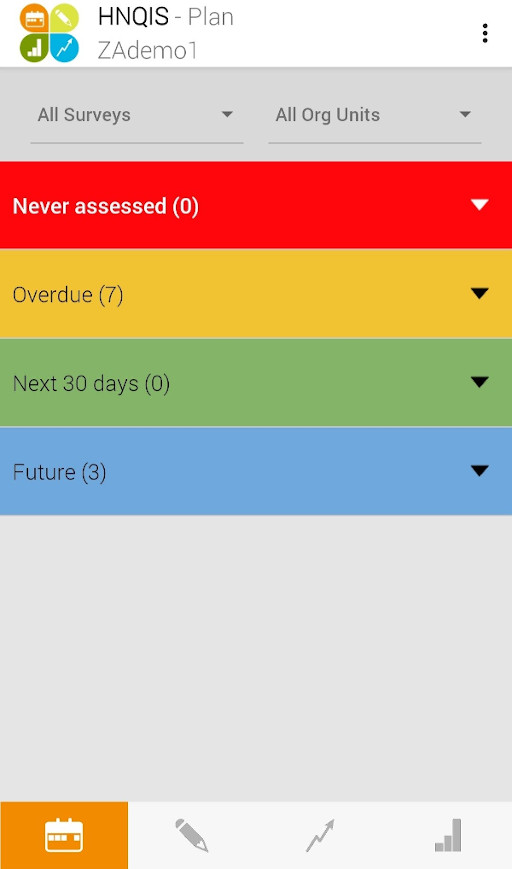
\includegraphics{images/hnqis-plan.jpg}
\textgreater{}The Date of next visit is automatized according to productivity (High/Low) and Quality of Care (QoC) score.

\begin{enumerate}
\def\labelenumi{\arabic{enumi}.}
\setcounter{enumi}{3}
\tightlist
\item
  The second page is \texttt{Assess\ module} which has customized checklists for assessing the facility and work environment.
\end{enumerate}

\begin{figure}
\centering
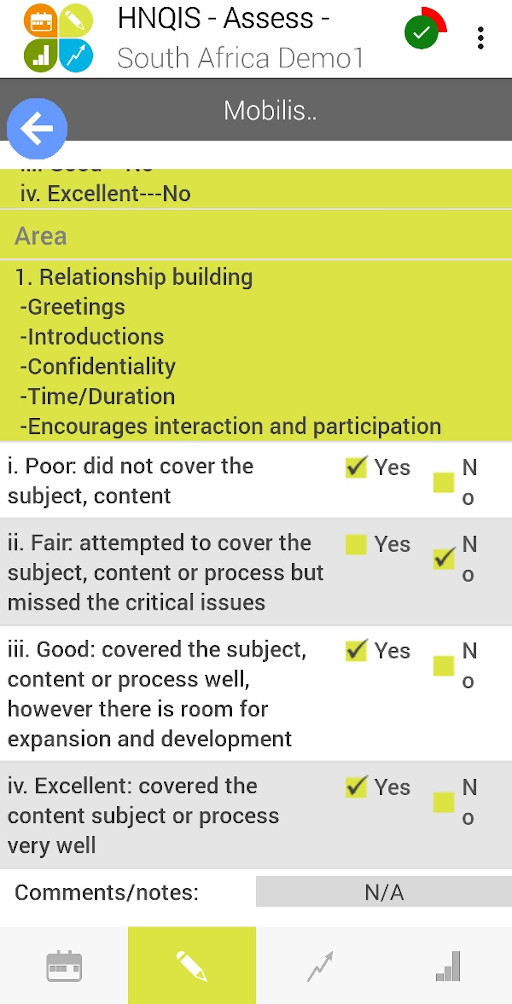
\includegraphics{images/hnqis-assess.jpg}
\caption{HNQIS Assess}
\end{figure}

\begin{quote}
Y/N answers allow for objectivity while assessing facilities' performance.
\end{quote}

\begin{enumerate}
\def\labelenumi{\arabic{enumi}.}
\setcounter{enumi}{4}
\tightlist
\item
  Next is the \texttt{Improve\ Module} that gives a quick identification of failed questions and critical gaps.
  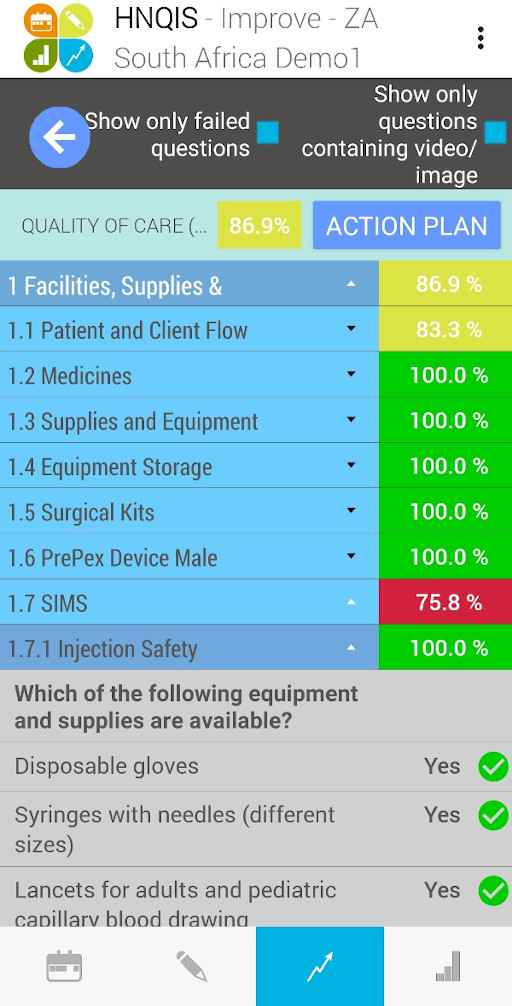
\includegraphics{images/hnqis-improve.jpg}
\end{enumerate}

\begin{quote}
The feedback scripts are in line with global guidelines. The standardized feedback reduces District Health Teams subjectivity.
\end{quote}

\begin{enumerate}
\def\labelenumi{\arabic{enumi}.}
\setcounter{enumi}{5}
\tightlist
\item
  Last is the \texttt{Monitor\ Module}, there is a quick overview of District Health Teams performance in terms of assessments and an overview of the QoC scores by health area and by org unit.
\end{enumerate}

\begin{figure}
\centering
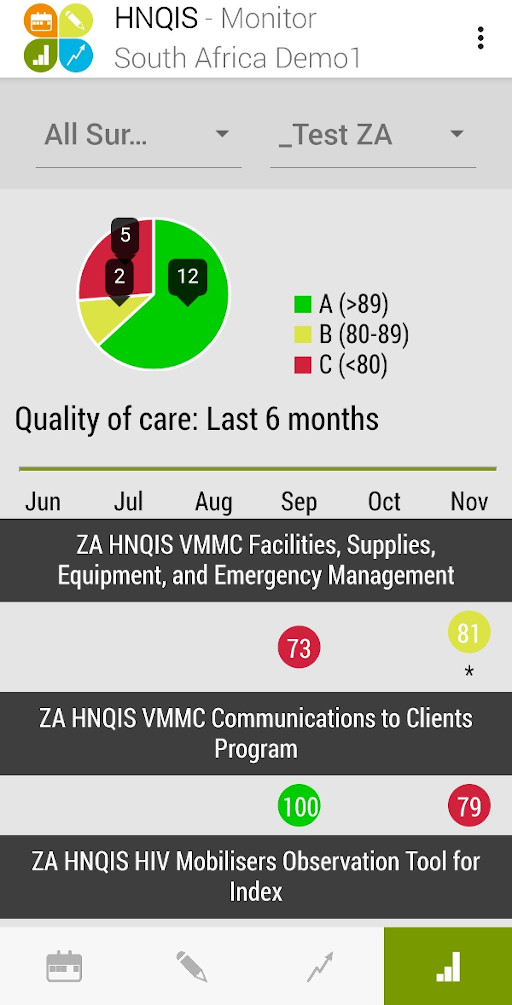
\includegraphics{images/hnqis-monitor.jpg}
\caption{HNQIS Monitor}
\end{figure}

To learn more about HNQIS, please visit the IM Data Hub help desk:
* \href{https://imdatahub.freshdesk.com/en/support/solutions/articles/47001032548-getting-started-on-hnqis}{Getting Started on HNQIS (English)}
* \href{https://imdatahub.freshdesk.com/fr/support/solutions/articles/47001032548-getting-started-on-hnqis}{Getting Started on HNQIS (French)}

\hypertarget{trouble}{%
\chapter{Getting Help on the IM Data Hub}\label{trouble}}

\hypertarget{im-data-hub-help-desk}{%
\section{IM Data Hub Help Desk}\label{im-data-hub-help-desk}}

\hypertarget{introduction-5}{%
\subsection{Introduction}\label{introduction-5}}

IM Data Hub is linked to a help desk system, IM Data Hub Help Desk, a platform where end users can get information and support on a specific service.

The Help Desk provides information, support and troubleshooting services to the IM Data Hub users. It helps the users and system admins communicate with system administrators more easily.

\hypertarget{services-offered}{%
\subsection{Services offered}\label{services-offered}}

\begin{enumerate}
\def\labelenumi{\arabic{enumi}.}
\tightlist
\item
  Submit a ticket for any issue you are experiencing on the IM Data Hub.
\item
  View the status of your submitted tickets to track progress on their resolution.\\
\item
  Learn how to handle tasks through the knowledge base articles from the solutions page.
\item
  Request for new features and functionality.
\item
  Search for answers for frequently asked questions (FAQs) on the IM Data Hub.
\item
  Keep up to date on the IM Data Hub by following announcements via the forum.
\end{enumerate}

\hypertarget{getting-started-with-im-data-hub-help-desk}{%
\subsection{Getting started with IM Data Hub Help Desk}\label{getting-started-with-im-data-hub-help-desk}}

To access the IM Data Hub Help Desk, please click any on the link below:

\begin{itemize}
\tightlist
\item
  English \url{https://imdatahub.freshdesk.com/en/support/home}
\item
  French \url{https://imdatahub.freshdesk.com/fr/support/home}
\end{itemize}

The help desk can also be accessed through the IM Data Hub as outlined below:

\begin{enumerate}
\def\labelenumi{\arabic{enumi}.}
\item
  Click on your initials.
  
\includegraphics{images/initials.png}
\item
  Click on the ``Help'' app.
  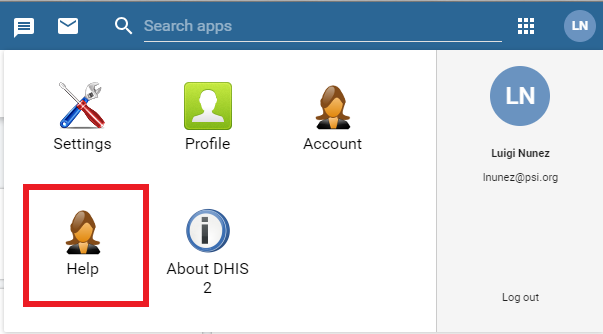
\includegraphics{images/help-menu.png}
\end{enumerate}

\hypertarget{creating-a-ticket}{%
\subsection{Creating a ticket}\label{creating-a-ticket}}

If you have an issue or a request, please use the steps below to create a ticket

\begin{enumerate}
\def\labelenumi{\arabic{enumi}.}
\tightlist
\item
  Access the help desk by clicking on the link below:

  \begin{itemize}
  \tightlist
  \item
    \href{https://imdatahub.freshdesk.com/en/support/tickets/new}{Create a ticket (English)}
  \item
    \href{https://imdatahub.freshdesk.com/fr/support/tickets/new}{Create a ticket (French)}
  \end{itemize}
\item
  Fill in the ticket details as per the form:
  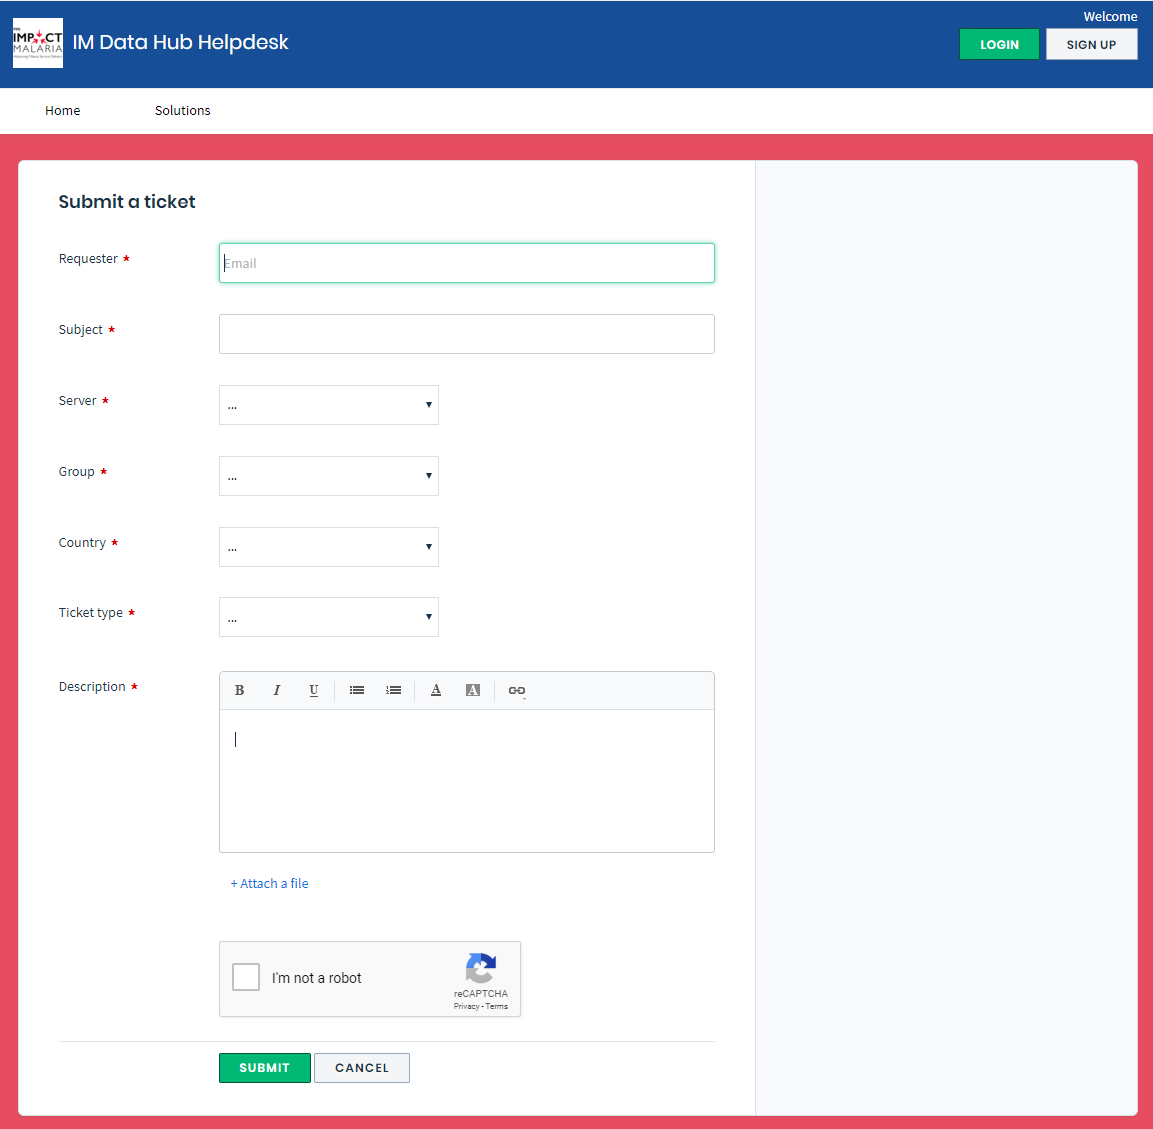
\includegraphics{images/ticket.png}
\end{enumerate}

\begin{itemize}
\tightlist
\item
  \textbf{Requester:} Enter your email address
\item
  \textbf{Subject:} Write the subject of your ticket
\item
  \textbf{Server:} choose the server on which you are experiencing the issue on
  * dev.imdatahub.org for the development server
  * imdatahub.org for the production server
\item
  \textbf{Group:}

  \begin{itemize}
  \tightlist
  \item
    \textbf{Generic} for IM Data Hub issues
  \item
    \textbf{HNQIS} for HNQIS specific issues
  \end{itemize}
\item
  \textbf{Country:} specify your country or select NA if not applicable
\item
  \textbf{Ticket type:} choose \textbf{Configuration}, \textbf{Maintenance}, \textbf{Question}, \textbf{Bug} or \textbf{Other} depending on the ticket type
\item
  \textbf{Description:} Please describe your issue in detail
\item
  \textbf{Attach a file:} Please use this to upload relevant files or screenshots to assist in resolving the issue
\end{itemize}

\hypertarget{references}{%
\chapter*{References}\label{references}}
\addcontentsline{toc}{chapter}{References}

\begin{enumerate}
\def\labelenumi{\arabic{enumi}.}
\item
  DHIS2 Developers guide
  \url{https://docs.dhis2.org/master/en/developer/html/dhis2_developer_manual.html}
\item
  DHIS2 Implementers guide
  \url{https://docs.dhis2.org/2.30/en/user/html/dhis2_user_manual_en_full.html}
\item
  IMPACT Malaria
  \url{https://impactmalaria.org/}
\end{enumerate}

\bibliography{book.bib,packages.bib}

\end{document}
